\documentclass[11pt]{article}
\usepackage[T1]{fontenc}
\usepackage[utf8]{inputenc}
\usepackage{lmodern}
\usepackage{microtype}
\usepackage[margin=1in]{geometry}
\usepackage{setspace}
\usepackage{amsmath,amssymb,amsthm}
\usepackage{mathtools}
\usepackage{bm}
\usepackage{graphicx}
\usepackage{booktabs}
\usepackage{tabularx}
\usepackage{array}
\usepackage{enumitem}
\usepackage{xcolor}
\usepackage{caption}
\usepackage{subcaption}
\usepackage{tikz}
\usetikzlibrary{arrows.meta,positioning,calc,decorations.pathreplacing}
\usepackage[authoryear,round]{natbib}
\usepackage{xurl}
\usepackage{xr}
\usepackage[hidelinks]{hyperref}
\usepackage{cleveref}

\theoremstyle{plain}
\newtheorem{proposition}{Proposition}
\newtheorem{lemma}{Lemma}
\newtheorem{corollary}{Corollary}
\theoremstyle{definition}
\newtheorem{assumption}{Assumption}
\newtheorem{definition}{Definition}
\theoremstyle{remark}
\newtheorem{remark}{Remark}

\crefname{proposition}{Proposition}{Propositions}
\crefname{lemma}{Lemma}{Lemmas}
\crefname{corollary}{Corollary}{Corollaries}
\crefname{assumption}{Assumption}{Assumptions}
\crefname{remark}{Remark}{Remarks}
\crefname{definition}{Definition}{Definitions}
\crefname{section}{Section}{Sections}
\crefname{subsection}{Section}{Sections}
\crefname{appendix}{Appendix}{Appendices}
\crefname{subappendix}{Appendix}{Appendices}
\crefname{table}{Table}{Tables}
\crefname{figure}{Figure}{Figures}
\crefname{equation}{equation}{equations}
\creflabelformat{equation}{(#2#1#3)}


\newcommand{\pos}[1]{\left[#1\right]^{+}}
\setlist{itemsep=2pt,topsep=4pt}

\externaldocument{main}
\onehalfspacing

\renewcommand{\thesection}{S\arabic{section}}
\renewcommand{\theproposition}{S\arabic{proposition}}
\renewcommand{\thelemma}{S\arabic{lemma}}
\renewcommand{\thecorollary}{S\arabic{corollary}}
\renewcommand{\theremark}{S\arabic{remark}}
\renewcommand{\thedefinition}{S\arabic{definition}}
\renewcommand{\theassumption}{S\arabic{assumption}}
\renewcommand{\thetable}{S\arabic{table}}
\renewcommand{\thefigure}{S\arabic{figure}}
\renewcommand{\theequation}{S\arabic{equation}}

\title{Online Supplement to ``Owning the Chokepoint: ASML, Alliance Dependence, and the Limits of Europe's Leverage over Washington''}
\author{Matt DiGiuseppe \and Claude (Anthropic)}
\date{\today}

\begin{document}
\maketitle

\noindent This supplement states the extensions that the article summarizes in \cref{sec:extensions}, describes the earlier cases behind \cref{sec:cases}, proves every result, reports the numerical checks, and reads the \emph{Europe 2031} scenario against the model. References to sections, results, figures and equations without an S are to the article.

\section{Notation}\label{app:notation}

\Cref{tab:notation} collects the notation of the baseline model in \cref{sec:model}. Symbols introduced in the extensions are defined where they are used.

\begin{table}[h]
\centering
\small
\caption{Notation for the baseline model}\label{tab:notation}
\begin{tabularx}{\textwidth}{@{}l>{\raggedright\arraybackslash}Xl>{\raggedright\arraybackslash}X@{}}
\toprule
Symbol & Meaning & Symbol & Meaning\\
\midrule
$E,U,C$ & Europe, United States, China & $a\in\{A,X\}$ & Atlantic alignment or exit\\
$V$ & US loss from exit, net of flow jurisdiction (dependence) & $W$, $\theta$ & China's gain from exit; share blocked by US flow jurisdiction\\
$\rho$ & China's relative-gains weight & $W_C$ & most China would pay, $(1-\theta)W+\rho V$\\
$\bar m_U,\bar m_C$ & largest stake on one commitment & $\lambda_C$ & Europe's value of a unit of China's promise\\
$\omega$ & China's credible offer, \cref{eq:omega} & $x_j(a)$, $d_j$ & provision of instrument $j$; its conditional part\\
$s_0$, $s_B$ & US own interest in European security; access value & $s_L$ & added US value of a loyal ally\\
$s_A$, $s_X$ & US stake in defending a loyal, realigned Europe & $m_S$ & US stake on abandoning a realigned Europe\\
$G$, $g$ & distribution and density of crisis costs $\xi$ & $\kappa$, $\bar\kappa$ & conditionality of the core guarantee, \cref{eq:kappa}; its maximum\\
$S_k$ & Europe's crisis-weighted stake in core defence & $d_p$, $d_{ai}$ & conditional parts of posture and of the AI instrument\\
$f$, $\gamma$, $c_f$ & firm penalty; US denial benefit; self-harm per unit of $V$ & $\chi_f$ & credibility of firm penalties\\
$\eta$ & Europe's intrinsic cost of exit & $c$ & credible cost of exit\\
$Q$ & exit premium, \cref{eq:Q} & $\Lambda$ & slack, $\pos{-Q}$\\
$\beta$ & Europe's probability of proposing & $\lambda$, $\phi$, $r$ & rupture hazard; repair rate; discount rate\\
$\psi$ & rupture weight, $\lambda/(\lambda+r+\phi)$ & $P^*$ & equilibrium transfer flow to Europe\\
$\bar b_C$ & China's credibility bound, $\lambda_C\bar m_C-c$ & $\mathcal P(q)$ & settlement at premium $q$ (\cref{sec:slack})\\
\bottomrule
\end{tabularx}
\end{table}

\section{Counter-Threats, Hedges and Conditionality}\label{app:counter}

This section gives the formal results on Chinese counter-threats, US policing of a hedge and Washington's choice of conditionality, which the main text summarizes in \cref{sec:linkref,sec:extensions}.

\subsection{Counter-threats and hedges}\label{sec:counter}

As in \cref{sec:security}, Chinese coercion enters only as counter-threats attached to particular concessions, announced before Washington makes its demands. We also consider a hedge, legacy-tool sales and servicing worth $y_H$ to Europe and $w_H$ to Washington if stopped: Washington can demand that Europe stop it, backed by $J^c$ (linkage), or threaten to block the hedged flows with its own jurisdiction, at net ex post cost $e_F$.

\begin{proposition}[Counter-threats and hedges]\label{prop:counter}
Maintain the assumptions of \cref{prop:slack} in the bidding benchmark.
\begin{enumerate}[label=(\alph*)]
\item \emph{Counter-threats.} Before the United States moves, China chooses credible counter-threats $r_k\in[0,\bar r_k]$. If concession $k$ is made and $r_k>0$, China executes at cost $e^C_k>0$ and Europe bears the sunk loss $r_k$. China loses $z_k\ge 0$ when concession $k$ is made. The United States makes a single ultimatum backed by $J^c$, and its optimal bundle is unique at the profiles compared below.
  \begin{enumerate}[label=(\roman*)]
  \item A counter-threat adds $r_k$ to the sunk cost of $k$: Europe accepts $S$ if and only if
  \[ \min\{T_{\mathrm r}(S),\Lambda\}+T_{\mathrm s}(S)+\textstyle\sum_{k\in S}r_k\le B(J^c). \]
  \item China does better than with no threats only if the United States' demand set changes.
  \item If a counter-threat on $k$ is executed in China's optimal profile, then dropping it changes the United States' demand set to one that contains a demand outside the equilibrium set. China executes on path only to crowd out other demands, and this occurs for an open set of parameters.
  \item The United States' payoff is weakly lower under any profile of counter-threats.
  \item Europe's net loss is at most $B(J^c)$ with or without counter-threats. It equals $B(J^c)$ in both cases if the United States has a divisible sunk demand of positive value that China cannot threaten. The counter-threat then taxes the patron, not the holder. Otherwise Europe's loss can rise or fall.
  \end{enumerate}
\item \emph{Policing a hedge.} Stopping a hedge worth $y_H$ to Europe is a reversible concession. If it is the only demand, linkage stops the hedge if and only if $\min\{y_H,\Lambda\}\le B(J^c)$ and $w_H\ge\pos{y_H-\Lambda}$, where $w_H$ is its value to the United States. The United States then pays rent $\pos{y_H-\Lambda}$. Linkage is free only if $y_H\le\min\{\Lambda,B(J^c)\}$, and its free part $\min\{y_H,\Lambda\}$ vanishes as $Q\to 0$. A staked threat to block the hedge by flow jurisdiction, with net ex post cost $e_F$, is credible if and only if $e_F\le\bar m_U$. It leaves $Q$ unchanged and is never executed. Executing a conditional withdrawal $J$ raises Europe's premium to $Q+d(J)$.
\end{enumerate}
\end{proposition}

Part (a) changes who pays for Chinese coercion. By (a)(i) a counter-threat makes a concession more expensive for Europe exactly as a sunk cost would. If Washington has other demands that China cannot reach, it fills the budget with them, and Europe's loss stays at $B(J^c)$. Washington drops the demand China has made expensive for others it values less, so the counter-threat taxes the patron. China gains only by changing what Washington asks for (part (a)(ii)), and it carries out a threat only to crowd out another demand (part (a)(iii); \cref{app:proofs} gives an example on the equilibrium path). \Cref{sec:record} reads the Nexperia episode against that requirement.

Part (b) separates the slack logic from a coercer that prices each demand at a fixed cost of the cheapest credible instrument (\cref{sec:predictions}). The free part of linkage, $\min\{y_H,\Lambda\}$, shrinks as the premium rises toward zero, and beyond it Washington must pay rent. Flow jurisdiction does not depend on slack: it is credible whenever $e_F\le\bar m_U$ and leaves $Q$ unchanged. So linkage against a hedge worth less to Washington than to Europe ($w_H<y_H$) should appear when the ally has slack and fade as its premium approaches zero, while the use of flow jurisdiction should not track the premium at all. A cost minimizer that counted the rent as a cost of linkage would predict the same switch.

Given our reading that Europe's premium has been negative since 2019 (\cref{sec:evidence}), the record is consistent with the first half of this prediction. The 2025 National Security Strategy and the August 2025 joint statement tie favourable treatment and US AI exports to export-control alignment (\cref{sec:background}), a reversible concession. The second half needs variation in premia that the Dutch record alone does not supply (\cref{sec:tests}).

\subsection{Conditionality as a choice}\label{sec:conditionality}

Washington chooses its conditionality. With $\kappa=G(s_A)-G(s_X-m_S)$ from \cref{eq:kappa}, choosing the stake $m_S\le\bar m_U$ is choosing $\kappa\in[\kappa_0,\bar\kappa]$, where $\kappa_0=G(s_A)-G(s_X)$ is the conditionality with no stake and $\bar\kappa$ is the largest Washington can create. Raising $\kappa$ lowers Europe's premium by $S_k$ per unit. If Washington converts slack into concessions worth $\nu\in[0,1]$ per unit of European cost, and conditionality has a convex cost $H(\kappa)$ in allied assurance, \cref{prop:conditionality} below characterizes its choice. A patron with no further demands ($\nu=0$) makes its guarantee just conditional enough to hold the premium at zero, or less if assurance becomes too costly first. Conditionality beyond that point is worth buying only because slack can be spent, so only a patron that plans to make demands makes its guarantee more conditional than the rivalry with China requires. When assurance is cheap at the margin, Washington answers a stronger Chinese offer by making its guarantee more conditional, by exactly enough to keep the premium at zero, and pays nothing. We read the favourable treatment that the National Security Strategy offers aligning countries this way (\cref{sec:counter,sec:coding}).

The assurance cost need not be assumed. Allies that doubt the patron build capabilities of their own \citep{lanoszka2018atomic}, and a guarantee tied to Europe's conduct can be triggered by mistake, so a second ally values its own alignment less when it sees Washington's guarantee to Europe made conditional.

\begin{remark}[A source of assurance cost]\label{rem:assurance}
Let a second ally's premium rise with Europe's conditionality, $Q_2(\kappa)=Q_2^0+a(\kappa-\kappa_0)$ with $a\ge 0$ and $Q_2^0\le 0$, and let Washington convert that ally's slack at the same rate $\nu$. Then $H(\kappa)=\Pi_2(\kappa_0)-\Pi_2(\kappa)$, with $\Pi_2=-\pos{Q_2}+\nu\pos{-Q_2}$, is nondecreasing and convex with $H(\kappa_0)=0$, so \cref{prop:conditionality} applies. Let $\tilde\kappa=\kappa_0-Q_2^0/a$ be the conditionality at which the second ally's premium reaches zero. If Europe's premium is negative at $\kappa_0$ and $\nu>0$, an optimal conditionality is $\kappa^*=\kappa_0$ if $a\ge S_k$, $\kappa^*=\min\{\tilde\kappa,\bar\kappa\}$ if $\nu S_k\le a<S_k$, and $\kappa^*=\bar\kappa$ if $a<\nu S_k$ (with $\tilde\kappa=\infty$ if $a=0$).
\end{remark}

Conditionality toward one ally spends the slack of the others. Washington makes Europe's guarantee more conditional only if Europe's stake in it, $S_k$, exceeds the spillover $a$ onto the second ally, and it stops where that ally's premium reaches zero unless the spillover is small even relative to the value of Europe's concessions. A patron with many allies watching makes its guarantees less conditional than one bargaining with a single holder.

An untargeted drawdown, such as the cut of 25,000 or more troops from Europe that NBC News reported in September 2026 the Pentagon was weighing \citep{nbc2026pentagon}, lowers what Washington provides to a loyal ally, $x_p(A)$, and with it $d_p$ and Europe's slack. The May 2026 order moving troops out of Germany (\cref{sec:background}) punished an act with no prior demand, which lies outside our demand-and-threat structure. Read as the execution of an implicit threat, it spends the instrument (\cref{sec:slackprinciple}) and raises the target's premium by the instrument's conditional part (\cref{prop:counter}(b)). Carrying it out at all requires the burning logic described after \cref{prop:slack}, or incomplete information as in \cref{prop:refusal}, and its effect on other allies' beliefs about $\kappa$ is what \cref{rem:assurance} prices.

The silicon shield, the fourth channel of \cref{cor:master}(e), has no fixed sign. If holding the chokepoint raises Washington's stake in Europe's security whatever Europe's alignment, $s_X$ rises. Where $G$ is unimodal with its mode at or below $s_X-\bar m_U$, so that the most likely crisis costs lie below Washington's net stake in a Europe that has exited, a higher $s_X$ lowers the most conditionality Washington can create (\cref{prop:conditionality}(d)). Where a staked abandonment makes defence of an exiter unlikely, $s_X-\bar m_U$ lies in the left tail of $G$, where the density rises, and holding the chokepoint can make the guarantee more conditional. \citet{blankenship2021price} finds that allies in locations the United States values contribute less to the common burden, which is what the first case implies.

\subsection{The conditionality proposition}\label{app:conditionality}

This subsection states the result discussed in \cref{sec:conditionality}. Choosing the stake $m_S\le\bar m_U$ is choosing $\kappa\in[\kappa_0,\bar\kappa]$, with $\kappa_0=G(s_A)-G(s_X)$ and $\bar\kappa$ as in \cref{eq:kappa}.

Conditionality is costly to the coercer, and we let it cost $H(\kappa)$, nondecreasing and convex with $H(\kappa_0)=0$ (\cref{rem:assurance} derives such a cost). The cost is one of assurance: other allies discount a guarantee that comes with a broad withdrawal rule, and a guarantee tied to Europe's conduct can be triggered by mistake. Allies that doubt the patron also build capabilities of their own \citep{lanoszka2018atomic}, which raises their premia and adds to $H$. With $Q_0$ the premium at $\kappa_0$, the premium is $Q(\kappa)=Q_0-(\kappa-\kappa_0)S_k$. Washington converts slack into concessions worth $\nu\in[0,1]$ per unit of European cost, a linear simplification of the concave value of capacity in \cref{cor:rationing}, and we assume $B(J^c)\ge\Lambda$ so that all slack can be converted. The bound $\nu\le 1$, which keeps the objective concave, says that a concession is worth less to Washington than it costs Europe; with $\nu>1$ Washington would buy concessions with rent. Washington chooses $\kappa$ before the bidding stage to maximize
\[
\Pi(\kappa)=-\pos{Q(\kappa)}+\nu\,\pos{-Q(\kappa)}-H(\kappa).
\]
Let $H'$ be the right derivative of $H$. For $x\ge 0$ let $\kappa_x=\inf\{\kappa\in[\kappa_0,\bar\kappa]:H'(\kappa)\ge x\}$, with $\inf\emptyset=+\infty$, and write $\kappa_1=\kappa_{S_k}$ and $\kappa_\nu=\kappa_{\nu S_k}$, so that $\kappa_0\le\kappa_\nu\le\kappa_1$. The conditionality at which the premium is exactly zero is $\kappa_z=\kappa_0+Q_0/S_k$.

\begin{proposition}[Conditionality is the price of concessions]\label{prop:conditionality}
The conditionality
\[ \kappa^*=\min\big\{\bar\kappa,\ \max\{\kappa_\nu,\ \min\{\kappa_z,\kappa_1\}\}\big\} \]
maximizes $\Pi$, uniquely if $H$ is strictly convex, and $Q(\kappa^*)=(\kappa_z-\kappa^*)S_k$.
\begin{enumerate}[label=(\alph*)]
\item If $\nu=0$, then $\kappa^*=\kappa_0$ when $Q_0\le 0$, and $\kappa^*=\min\{\kappa_z,\kappa_1,\bar\kappa\}$ otherwise. The United States never makes its guarantee more conditional than needed to hold the premium at zero. It creates no slack: $\Lambda^*=\pos{-Q_0}$.
\item If $\nu>0$, $\kappa_0\le\kappa_z<\bar\kappa$ and $H'(\kappa_z)<\nu S_k$, then $\kappa^*=\min\{\kappa_\nu,\bar\kappa\}>\kappa_z$ and $\Lambda^*=(\kappa^*-\kappa_z)S_k>0$: conditionality is the price of concessions. If $Q_0<0$, then $\kappa^*=\min\{\kappa_\nu,\bar\kappa\}$ and $\Lambda^*=(\kappa^*-\kappa_z)S_k\ge -Q_0$.
\item Let $H$ be strictly convex and differentiable. Away from regime boundaries:
  \begin{enumerate}[label=(\roman*)]
  \item if $\kappa^*=\kappa_z$, then $d\kappa^*/dQ_0=1/S_k$ and the United States pays no rent: a stronger Chinese bid elicits a more conditional guarantee, not a payment;
  \item if $\kappa^*=\kappa_1<\min\{\kappa_z,\bar\kappa\}$ (assurance is costly at the margin before the premium reaches zero), $\kappa^*$ does not depend on $Q_0$ and the rent $Q(\kappa_1)>0$ rises one for one with $Q_0$;
  \item if $\kappa^*=\kappa_\nu\in(\max\{\kappa_z,\kappa_0\},\bar\kappa)$, or if $\kappa^*=\kappa_0>\kappa_z$, then $\kappa^*$ does not depend on $Q_0$ and slack falls one for one with $Q_0$: China's bid is paid for out of the United States' concessions;
  \item if $\kappa^*=\bar\kappa$, the United States pays $\pos{Q(\bar\kappa)}$, which rises one for one with $Q_0$ when $Q(\bar\kappa)>0$. Otherwise slack falls one for one.
  \end{enumerate}
\item $d\bar\kappa/ds_X=g(s_X+s_L)-g(s_X-\bar m_U)$, with $s_L$ and $\bar m_U$ fixed. Hence $\bar\kappa$ is nonincreasing in $s_X$ wherever $g$ is nonincreasing on $[s_X-\bar m_U,\,s_X+s_L]$, for example when $G$ is unimodal with its mode at or below $s_X-\bar m_U$, and it is then nonincreasing in the access value of European territory and, if $s_B$ rises with $V$, in $V$. If instead $g(s_X+s_L)>g(s_X-\bar m_U)$, $\bar\kappa$ rises with $s_X$. If $s_A$ is held fixed when $s_X$ rises, $\bar\kappa$ is nonincreasing in $s_X$ for every $G$.
\end{enumerate}
\end{proposition}

\section{Control Rights and Preventive Demands}\label{sec:control}

The static model holds Europe's exit premium fixed. Yet the premium moves: Chinese offers and European rearmament raise it, and Chinese indigenization lowers it. A Washington that expects it to turn positive expects to pay rents that Europe cannot credibly promise to forgo. A transfer of control can remove them.

\subsection{Setup}\label{sec:controlsetup}

There are two periods, $t\in\{1,2\}$, and a discount factor $\delta\in(0,1]$. In each period in which Europe holds control, the bidding contest of \cref{lem:bidding} is played at that period's premium $Q_t$, and Europe receives $\pos{Q_t}$. We assume that Washington retains Europe at every contest, including after a cut ($Q_1+d_1<V$ and $Q_1+d_1\le\bar m_U$, and the same in period 2 at the highest premium Europe can reach), and that payments are made at signing.

\paragraph{The ultimatum.} At the start of period 1, before the period-1 contest, Washington may issue an ultimatum at an issuing cost $\iota\ge 0$: Europe transfers control of ASML's customers, output and technology for both periods against a payment $T\ge 0$, or Washington withdraws a bundle $J$ of instruments for period 1. The bundle has unconditional part $u_1$, conditional part $d_1$ and direct ex post cost $g_1\ge 0$ to Washington (\cref{sec:commitment}). If Europe refuses and the threat is carried out, Europe's premium rises to $Q_1+d_1$, and by \cref{prop:slack}(a) the refusal costs Europe the bite
\[
B_1=u_1+\min\{d_1,\Lambda_1\},\qquad \Lambda_1=\pos{-Q_1},
\]
net of the rent Washington must then pay. Carrying out the threat costs Washington $e=g_1+\pos{Q_1+d_1}-\pos{Q_1}$, its direct cost plus the extra rent. The threat is credible if and only if $e\le\bar m_U$; otherwise $B_1=0$. We assume that no other period-1 demand draws on the bite; with other demands, control enters \cref{cor:rationing} as a sunk demand.

We do not expect the core guarantee to back such an ultimatum. Withdrawing protection from a Europe that stays aligned costs Washington its own stake in defending a loyal ally, so $g_1$ is large unless $s_A$ is small. Posture, enablers and the AI instrument cost less to withdraw for one period.

\paragraph{Control.} A transfer lowers Europe's premium at both dates by $\Delta_c\in(0,\infty]$, the enforceability of control. With $\Delta_c=\infty$ Europe can never again choose exit. With $\Delta_c$ finite, a Europe whose premium later rises far enough could take back part of what it gave. What is transferred sets $\Delta_c$. Relocating capacity to US soil raises it, and so does control exercised through ASML's US subsidiaries, which are US-law entities \citep{asml2026subsidiaries}. A controlling vote in a Dutch holding company stays under Dutch law and has low $\Delta_c$; we think it would be exposed to emergency powers like the Goods Availability Act order against Nexperia of 30 September 2025 \citep{kst32637720}.

\paragraph{Values and costs.} Washington places an intrinsic value $v_c\ge 0$ on control, apart from the rents it saves. Europe bears a sovereignty cost $\sigma\ge 0$ if it transfers control. It includes the domestic cost of surrendering a national champion and hurdles fixed in advance: ASML's foundation, which can acquire preference shares halving ordinary shareholders' votes \citep{asml2026annual}, notification duties under the Vifo Act \citep{nl2022vifo, nl2023sensitief}, and review under the Foreign Subsidies Regulation, which we infer a US-funded acquisition would trigger \citep{eu2022fsr}. Being public, these hurdles raise $\sigma$ before Washington decides whether to demand anything. China punishes a completed transfer with $r^c\ge 0$, which Europe bears.

\paragraph{Autonomy investment.} After the period-1 outcome, and before the period-2 contest, Europe can make an observable investment at cost $K$ that raises its period-2 premium by $\bar I$, for instance rearmament that lowers $S_k$. Holding a period-2 premium $q$, it invests if and only if $\delta(\pos{q+\bar I}-\pos{q})>K$.

\paragraph{Ties.} An indifferent Europe accepts; Washington issues only if it strictly gains (the limit $\iota\to 0^{+}$ when $\iota=0$); Europe invests only if that is strictly profitable. After a transfer Washington keeps its baseline provision, since withdrawing it would cost something and gain nothing.

\subsection{Preventive control}\label{sec:preventive}

Let $I(q)=\mathbf 1\{\delta(\pos{q+\bar I}-\pos{q})>K\}$ indicate investment at period-2 premium $q$. Washington's discounted period-2 rent is $\mathrm{Rent}_U(q)=\delta\pos{q+\bar I\,I(q)}$, and Europe's period-2 value net of its investment cost is $\mathrm{Val}_H(q)=\mathrm{Rent}_U(q)-K\,I(q)$.

\begin{proposition}[Preventive control]\label{prop:control}
Let
\begin{align*}
\Delta R_U&=\pos{Q_1}-\pos{Q_1-\Delta_c}+\mathrm{Rent}_U(Q_2)-\mathrm{Rent}_U(Q_2-\Delta_c),\\
\Delta R_H&=\pos{Q_1}-\pos{Q_1-\Delta_c}+\mathrm{Val}_H(Q_2)-\mathrm{Val}_H(Q_2-\Delta_c).
\end{align*}
Let $B_1=u_1+\min\{d_1,\Lambda_1\}$ if the threat is credible ($e\le\bar m_U$, with $e=g_1+\pos{Q_1+d_1}-\pos{Q_1}$) and $B_1=0$ otherwise. In the subgame-perfect equilibrium, the United States issues the ultimatum, and Europe accepts, if and only if
\begin{equation*}
\Gamma\equiv v_c-\iota+\min\{\Delta R_U,\;(\Delta R_U-\Delta R_H)+B_1-\sigma-r^c\}>0 .
\end{equation*}
The payment is $T^*=\pos{\Delta R_H-B_1+\sigma+r^c}$, the United States gains $\Gamma$, and Europe's payoff is
$\max\{\Delta R_H-B_1,\,-\sigma-r^c\}+\pos{Q_1-\Delta_c}+\mathrm{Val}_H(Q_2-\Delta_c)$.
An ultimatum that is issued is accepted. The credibility condition $e\le\bar m_U$ does not depend on $\Delta_c$.
\end{proposition}

The proof is in \cref{app:proofs}. $\Delta R_U$ is the rent that control saves Washington and $\Delta R_H$ is what Europe gives up by losing it; they differ only by the investment cost a transfer spares Europe. Washington gains the value of control net of the issuing cost, plus the smaller of the rent saved and what it can extract by force. Europe is paid for the rents it surrenders and the deadweight cost $\sigma+r^c$, less the bite. A refused ultimatum never pays Washington, so the threat is never carried out on the path. Its credibility is judged against a Europe that keeps control, which is why $\Delta_c$ does not enter.

In the special case $v_c=\iota=0$, $\Delta_c=\infty$, $\bar I=0$ and $Q_1<0$, the gain is $\Gamma=\min\{\delta\pos{Q_2},\,B_1-\sigma-r^c\}$. Washington demands control if and only if Europe's future premium is positive and the bite exceeds $\sigma+r^c$. Since $B_1\le u_1+\Lambda_1$, a purely conditional bundle clears that bar only if $Q_1<-(\sigma+r^c)$. The demand comes while Europe is weak but expected to grow stronger.

\begin{corollary}[Motive, investment, enforceability, China]\label{cor:control}
\leavevmode
\begin{enumerate}[label=(\alph*)]
\item \emph{Preventive motive.} $\Gamma>0$ if and only if $\Delta R_U>\iota-v_c$ and $B_1+(\Delta R_U-\Delta R_H)>\sigma+r^c+\iota-v_c$. If $v_c\le\iota$, issuance requires $\Delta R_U>0$ and $B_1+(\Delta R_U-\Delta R_H)>\sigma+r^c$. For $\Delta_c>0$, $\Delta R_U>0$ if and only if $Q_1>0$ or $Q_2+\bar I\,I(Q_2)>0$: Europe's premium is positive at date 1, or its premium after its own investment is positive at date 2.
\item \emph{Autonomy investment.} $\Delta R_U-\Delta R_H=K\,[I(Q_2)-I(Q_2-\Delta_c)]\ge 0$. Both arguments of the minimum in $\Gamma$ are weakly larger than when Europe has no investment option ($\bar I=0$), so an autonomy investment that Europe cannot commit to forgo weakly raises $\Gamma$. With investment, the United States can obtain control with no bite at all: if $B_1=0$, the ultimatum is issued if and only if $\Delta R_U>\iota-v_c$ and $K[I(Q_2)-I(Q_2-\Delta_c)]>\sigma+r^c+\iota-v_c$, and the transfer then saves Europe's investment cost.
\item \emph{Enforceability.} Holding $\sigma$, $r^c$, $v_c$ and $\iota$ fixed, $\Gamma$ and $T^*$ are nondecreasing in $\Delta_c$; $B_1$ and the credibility condition do not depend on $\Delta_c$.
\item \emph{Counter-threats against a transfer.} Before the United States decides, China announces a punishment $r^c\in[0,\bar r^c]$ of a transfer and a stake $m_C\le\bar m_C$. Carrying out $r^c$ after a transfer has ex post value $-e^C(r^c)$ to China, where $e^C$ is continuous and increasing with $e^C(0)=0$; the threat is credible if and only if $e^C(r^c)\le m_C$. China gets $z_C\ge 0$ if Europe keeps control, and the ex post payoff of its punishment decision ($-e^C(r^c)$ if it punishes, $-m_C$ if it does not) if control passes. Write $\Gamma(r^c)$ for $\Gamma$ at punishment $r^c$, and let $r^c_{\max}=\max\{x\le\bar r^c:e^C(x)\le\bar m_C\}$. In every subgame-perfect equilibrium:
\begin{enumerate}[label=(\roman*)]
\item if control is transferred, China does not punish: on the path the punishment is zero, the payment is $\pos{\Delta R_H-B_1+\sigma}$ and $\Gamma(0)>0$;
\item a credible punishment $r^c>0$ is announced only if it deters, $\Gamma(r^c)\le 0$;
\item if $z_C>0$, control is transferred if and only if $\Gamma(r^c_{\max})>0$; otherwise China deters with a credible $r^c\ge v_c-\iota+\Delta R_U-\Delta R_H+B_1-\sigma$ whenever $\Gamma(0)>0$;
\item if $z_C=0$ and $\Gamma(0)>0\ge\Gamma(r^c_{\max})$, both the transfer and its deterrence are equilibrium outcomes.
\end{enumerate}
If punishing is self-rewarding ($e^C(x)<0$ for some $x$), (i) fails: China may let the transfer happen and punish it.
\end{enumerate}
\end{corollary}

When $v_c=0$ and Europe has no autonomy investment that a transfer would forestall, an accepted transfer is inefficient. The rents it avoids are transfers between Washington and Europe, while the sovereignty cost and the issuing cost are destroyed, and China's punishment adds to the loss when, being self-rewarding, it is carried out (part (d)). That is the logic of preventive war \citep{fearon1995rationalist, powell2006war}, with a coerced transfer in place of a war. With an investment option the transfer can be efficient, because it spares Europe an investment cost $K$ sunk only to secure rents (part (b)), the one place where the logic of \citet{grossman1986costs} operates in our model. What our setting adds to the models of \cref{sec:literature} is a ceiling on coercion: the conditional part of the bite cannot exceed Europe's current slack, so the patron must act while the holder is weak.

Part (b) ties the demand to Europe's own choices. Rearmament, or any other investment in future bargaining power that Europe cannot commit to forgo, invites the demand, as an observable nuclear programme invites prevention or a deal \citep{debs2014known, spaniel2019bargaining}. It raises the rents a transfer saves and creates a surplus the two can share, which permits a purchase with no bite. Take $\delta=1$, $Q_1=1$, $Q_2=-\tfrac12$, $\bar I=3$, $K=2$, $\Delta_c=\infty$, $\sigma=1$ and $r^c=v_c=\iota=0$, with no threat. Europe would invest, so Washington faces a period-2 rent of $2.5$ on top of the period-1 rent of $1$. It buys control for $T^*=2.5$ and gains $\Gamma=1$; the transfer spares an investment of $2$ at a sovereignty cost of $1$.

By part (c), a transfer that Europe could partly undo removes only $\min\{\pos{Q_t},\Delta_c\}$ of the rent at each date, so the commitment problem returns whenever $Q_2-\Delta_c>0$, and Washington gains less and pays less, the buy-or-lease logic of \citet{harstad2016market}. Relocating production is the high-$\Delta_c$ end. The control rights Washington has taken so far all attach to assets on US soil, where enforcement does not depend on a foreign government: consent rights over the ownership, exit and customers of MP Materials, bought with equity, a price floor and an offtake \citep{mp2025dod}, a golden share in US Steel as a condition of its acquisition by Nippon Steel \citep{ussteel2025nsa}, and a passive stake in Intel \citep{intel2025agreement}. Toward Taiwan, Washington has sought relocation (\cref{sec:cases}).

By part (d), China's threat to punish a transfer is never carried out on the path: once control has passed, punishing costs China something and deters nothing. The threat protects European ownership only by deterring the demand, which requires $\Gamma(r^c_{\max})\le 0$. Sovereignty costs work the same way, which makes the hurdles of \cref{sec:controlsetup} part of Europe's protection against a demand.

The motive does not need Europe's premium to turn positive. It needs a surplus that Washington expects to pay and that a transfer would remove, and \cref{sec:slack} showed that rupture risk, hold-up and price driving all create such a surplus.

\begin{remark}[Control under a general settlement]\label{rem:controlsettle}
Replace the period-$t$ contest in \cref{prop:control} by a settlement $\mathcal P$ that satisfies (S1)--(S3) of \cref{sec:slackprinciple} and depends only on Europe's premium (so that a rupture after a partial transfer still costs Washington $V$), and let $\Delta_c$ be finite. Then \cref{prop:control} holds with $\mathcal P$ in place of $\pos{\cdot}$ throughout, with bite $B_1=u_1+d_1-[\mathcal P(Q_1+d_1)-\mathcal P(Q_1)]$ and execution cost $e=g_1+\mathcal P(Q_1+d_1)-\mathcal P(Q_1)$. If $\mathcal P$ is strictly increasing and convex, as under rupture risk with $\psi(1-\beta)>0$, then $\Delta R_U>0$ whatever the signs of $Q_1$ and $Q_2$.
\end{remark}

Take $\delta=1$, $Q_1=Q_2=-1$, bargaining under rupture risk with $V=4$, $\beta=0.5$, $\lambda=1$, $r=0.25$ and $\phi=0$ ($\psi=0.8$), $\Delta_c=2$, no investment, $\sigma=1$, $r^c=v_c=\iota=0$, and a purely conditional threat with $d_1=2$ and $g_1=0$, credible if $\bar m_U\ge 0.8$. Europe's price is $\mathcal P(-1)=1.2$ at each date and would be $\mathcal P(-3)=0.4$ after a transfer, so $\Delta R_U=1.6$. The bite is $B_1=2-(\mathcal P(1)-\mathcal P(-1))=1.2$, so $\Gamma=\min\{1.6,\,1.2-1\}=0.2>0$ and Washington buys control for $T^*=1.4$, although Europe's premium is negative at both dates. In the bidding benchmark the same parameters give $\Delta R_U=0$ and no demand. A full transfer ($\Delta_c=\infty$) differs: rupture can then no longer end in exit, so the settlement after a transfer is the status quo, $0$, and a transfer saves Washington $\mathcal P(Q_1)+\delta\mathcal P(Q_2)$. That is negative when rupture risk makes a weak Europe concede ($\mathcal P<0$), so owning the chokepoint outright would cost Washington the leverage that rupture risk gives it over a weak holder. For a convex $\mathcal P$, $\Gamma$ and $T^*$ still rise with finite $\Delta_c$, as in \cref{cor:control}(c), but under rupture risk $\mathcal P(Q_t-\Delta_c)$ falls without bound as $\Delta_c$ grows, so $T^*$ is unbounded over finite enforceability and drops at $\Delta_c=\infty$; monotonicity does not survive that jump.

\subsection{Windows}\label{sec:windows}

\Cref{prop:control} allows one ultimatum and a one-period cut. When a cut runs over several dates, its bite is the discounted sum of the per-date bites $u_s+\min\{d_s,\Lambda_s\}$, provided Washington retains Europe throughout and the cut leaves the premium at other dates unchanged (\cref{lem:selflimit} in \cref{app:cuts}). A cut is spent once executed, and extending a purely conditional cut into a date at which Europe's premium is positive adds nothing to its bite. A threat of permanent exclusion therefore bites no harder than one confined to the dates at which Europe has slack.

\begin{corollary}[Windows]\label{cor:windows}
Consider $N$ dates with $v_c=0$ and $\Delta_c=\infty$. At any date $t$ at which Europe still holds control, the United States may issue, at cost $\iota>0$, an ultimatum: transfer control for all remaining dates against a payment $T\ge 0$, or face a cut at date $t$ only, with bite $b_t=u_t+\min\{d_t,\Lambda_t\}$ and execution cost $e_t=g_t+\pos{Q_t+d_t}-\pos{Q_t}$. Call $t$ \emph{eligible} if $e_t\le\bar m_U$, $b_t>\sigma+r^c$, and $Q_{t'}>0$ for some $t'\ge t$. There is $\bar\iota>0$ such that for every $\iota\in(0,\bar\iota)$, the United States issues an ultimatum on the equilibrium path if and only if some date is eligible. Every ultimatum issued is accepted, and the first one comes no later than the last eligible date (possibly at a date that is not eligible). The same holds at $\iota=0$ when the United States issues only if it strictly gains. If $u_t=0$ at every date, the condition $t'\ge t$ can be replaced by $t'>t$.
\end{corollary}

\begin{figure}[t]
\centering
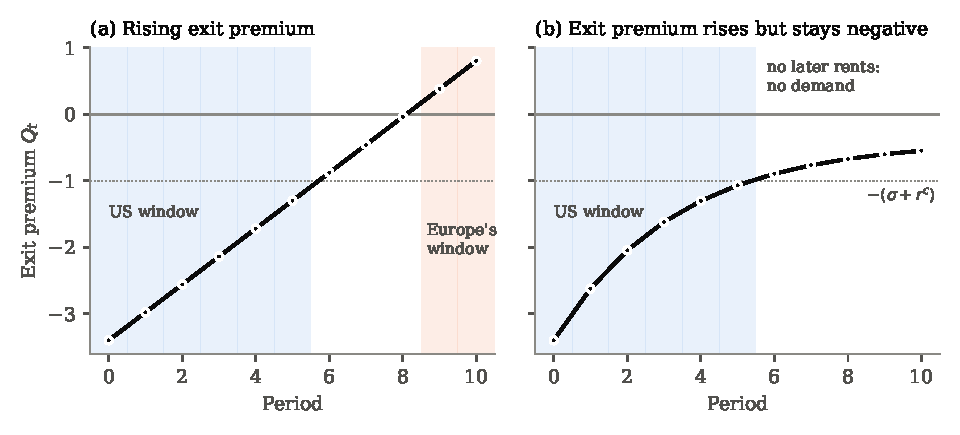
\includegraphics[width=0.95\textwidth]{figures/fig_windows.pdf}
\caption{Windows for preventive control (illustrative units). Panel (a): $Q_t=-3.4+0.42\,t$. Panel (b): $Q_t=-3.4+3(1-e^{-0.3t})$. In both, $\sigma+r^c=1$ and Washington holds a conditional instrument with $d_t=2$ and no unconditional part, so the condition $t'>t$ of \cref{cor:windows} applies; the cut is assumed credible at every date. Blue shading marks dates at which the threat bites by more than $\sigma+r^c$, which here requires $Q_t<-1$. Orange shading marks Europe's window, $Q_t>0$.}
\label{fig:windows}
\end{figure}

In panel (a) of \cref{fig:windows} the threat bites by more than $\sigma+r^c$ through $t=5$, and the premium turns positive at $t=9$. Washington acts at or before $t=5$, long before Europe's window opens. It can act earlier still, because a Europe that refuses remains exposed to a later demand (\cref{app:numerics} reports how often). In panel (b) the premium rises toward $-0.4$ but never crosses zero, and with $v_c=0$ Washington has nothing to prevent; with $v_c>\iota$ it could still demand control (\cref{cor:control}(a)).

In \citet{powell2006war} preventive war requires a shift in power that is large and rapid relative to what the declining state can be offered within the period. Here, under complete information, the speed of the shift affects when Washington acts and what it pays, and not whether it acts, because a transfer with $\Delta_c=\infty$ removes every future rent at once. With finite enforceability a shift far above $\Delta_c$ leaves rents that no transfer can reach, and size and speed matter again, as in Powell's account.

The direction of drift is therefore decisive. Rearmament and the rationing of loyal allies invite a demand, while Chinese indigenization, by lowering $W$, removes the motive. We cannot tell from the record which dominates.

\subsection{Promises or threats}\label{sec:bind}

Europe could instead remove the commitment problem itself, by binding itself against exit without transferring control. Binding also raises Europe's slack and with it the bite of Washington's threats.

\begin{remark}[Self-binding and dual key]\label{rem:bind}
Before period 1, Europe can adopt a binding rule (Europeanized or treaty-entrenched controls) that lowers its premium at both dates by $\Delta_b\in(0,\infty]$ at cost $\sigma^b$, drawing a Chinese punishment $r^b$; Europe keeps the key. The game of \cref{prop:control} is then played with premia $Q_t-\Delta_b$, and the bite of the US threat is computed at the new slack.
\begin{enumerate}[label=(\alph*)]
\item With $\Delta_b=\infty$, control removes no rents, and the bite becomes $B_1^b=u_1+d_1$ if $g_1\le\bar m_U$ (and $0$ otherwise). The United States then issues if and only if $\Gamma^b=v_c-\iota+\min\{0,\,B_1^b-\sigma-r^c\}>0$, so binding pre-empts the ultimatum if and only if $v_c\le\iota$ or $v_c-\iota+B_1^b\le\sigma+r^c$. If it does not, the United States demands control and pays $\pos{\sigma+r^c-B_1^b}$.
\item Let $Q_1<0$, $\Delta_c=\infty$, no investment and $\Delta_b=\infty$. Europe's payoff is $-\sigma^b-r^b-\mathbf 1\{\Gamma^b>0\}\min\{\sigma+r^c,B_1^b\}$ if it binds, and $\max\{\delta\pos{Q_2}-B_1,\,-\sigma-r^c\}$ if it does not bind and $\Gamma>0$, or $\delta\pos{Q_2}$ if it does not bind and $\Gamma\le 0$. In particular, if the United States would issue the ultimatum without binding and binding pre-empts it, Europe strictly prefers to bind if and only if $-\sigma^b-r^b>\max\{\delta\pos{Q_2}-B_1,\,-\sigma-r^c\}$. If the United States would not issue without binding, Europe never strictly prefers to bind.
\item A partial binding ($\Delta_b<\infty$) lowers the rents control would remove but raises the slack, hence the bite, so it can make $\Gamma$ positive. Example, with $\Delta_c=\infty$, no investment and $\bar m_U\ge 1$ (so that the cut is credible after binding): $\delta=1$, $Q_1=-1$, $Q_2=10$, $u_1=0$, $d_1=5$, $g_1=0$, $\sigma=1.5$, $r^c=v_c=\iota=0$. Without binding $\Gamma=\min\{10,\,B_1-1.5\}<0$ whether or not the cut is credible ($B_1=1$ if $\bar m_U\ge 4$ and $0$ otherwise). With $\Delta_b=3$, $\Gamma=\min\{7,\,4-1.5\}=2.5$ and the United States demands control at $T^*=4.5$.
\item Dual-key licensing is a partial control transfer with enforceability $\Delta_d<\infty$, sovereignty cost $\sigma_d<\sigma$, value $v_d$ and Chinese punishment $r^d$. If the United States can demand either arrangement, it demands the one with the larger of $\Gamma_{\mathrm{full}}$ and $\Gamma_{\mathrm{dual}}$ (each given by \cref{prop:control} with that arrangement's parameters), provided it is positive. Because $\sigma_d<\sigma$, the United States can obtain a dual key when the bite is too small to obtain full control.
\end{enumerate}
\end{remark}

Binding pre-empts a demand only if Washington values control little for its own sake, since full binding maximizes the bite and makes control cheaper to coerce for a patron with $v_c>\iota$. By part (b), binding pays Europe only when it pre-empts a demand that would otherwise come, at a lower cost. By part (c), a rule that binds Europe partway removes some of the rents Washington fears but adds to the slack its threats draw on, and can turn a demand that would not pay into one that does.

Washington can also demand binding itself. \Cref{prop:control} prices that demand with $(\Delta_b,\sigma^b,r^b)$ in place of $(\Delta_c,\sigma,r^c)$ and $v_c=0$, so a patron that values control little for its own sake prefers to demand binding whenever $\sigma^b+r^b<\sigma+r^c$. A preventive demand need not be a demand for ownership. Under binding Europe holds the only key. Under a dual key Washington holds a veto over China-bound licences, a control right over customers that \cref{rem:bind}(d) prices with its own enforceability and sovereignty cost. The Dutch government's opposition to the extraterritorial reach of the MATCH Act (\cref{sec:background}) suggests to us that $\sigma_d$ in The Hague is not far below $\sigma$, while parliament's October 2026 vote for harmonized EU export control suggests that $\sigma^b$ is low (\cref{sec:record}).

We read the European steps of 2024 and 2025 (\cref{sec:background}) as partial binding. When licensing of the NXT:1970i and NXT:1980i moved from Washington to The Hague in September 2024 \citep{stcrt2024duv}, Europe's premium fell and the key stayed in Europe, the reverse of a control transfer; \cref{sec:coding} codes the December 2024 Supplement No.~4 status as the matching reward for self-binding. On our reading, Delegated Regulation 2025/2003 \citep{eu2025dualuse} raised $\Delta_b$, because removing its entry takes an act at Union level that the Netherlands cannot adopt alone. It also had a US-facing cost. Listed tools ship to US fabs under the Union authorisation EU001 (\cref{sec:background}), so the Netherlands gave up a national licence over their US-bound shipments and, we think, part of Europe's hold-up option (\cref{sec:holdup}). None of these steps comes close to $\Delta_b=\infty$, and by part (c) they could have strengthened the US motive for a demand as easily as weakened it.

\subsection{Private sovereignty costs and breakdown}\label{sec:breakdown}

Under complete information an ultimatum is accepted or never issued. Breakdown requires that Washington be unsure what a transfer would cost Europe. We think that uncertainty is real: since February 2026 the Dutch cabinet has governed with minority support in parliament \citep{nltimes2026coalition, omroepbrabant2026kabinet}, so the domestic price of a transfer would depend on whichever majority it could find. When $\sigma$ is Europe's private information, a threat-backed ultimatum is refused with positive probability and the threat is carried out (\cref{prop:breakdown} in \cref{app:cuts}). Refusal is likelier when China's punishment of a transfer is credible and large, when Europe's future premium is high, and when the threat is cheap for Washington to carry out, the risk-return trade-off of \citet{fearon1995rationalist}. A patron that values control for its own sake may switch from a purchase offer to a threat as the bite rises, which can raise the probability of breakdown. These probabilities describe a patron that can commit to one public demand.

\subsection{Cuts and breakdown}\label{app:cuts}

\Cref{prop:control} allows one ultimatum and a cut that lasts one period. A threat of permanent exclusion withdraws instruments at many dates, and \cref{cor:windows} lets Washington issue ultimatums at several dates. The lemma below gives the bite and the cost of such a cut. Its two scope conditions push in opposite directions. If a cut drives Europe out at some date, Europe's loss exceeds the formula. If Europe responds to a cut it learns of in advance, for instance with the autonomy investment of \cref{sec:controlsetup}, the loss falls short of it.

\begin{lemma}[Spent and self-limiting cuts]\label{lem:selflimit}
Let dates $s=1,\dots,N$ have premia $Q_s$, slack $\Lambda_s=\pos{-Q_s}$ and discount factor $\delta$. A cut over a set $S$ of dates withdraws at each $s\in S$, before the date-$s$ contest, a bundle with unconditional part $u_s$, conditional part $d_s$ and direct ex post cost $g_s\ge 0$ to the United States. Suppose that at every $s\in S$ the United States still retains Europe after the cut ($Q_s+d_s<V_s$ and $Q_s+d_s\le\bar m_U$), and that the cut does not change the premium at any other date. Then:
\begin{enumerate}[label=(\roman*)]
\item the bite of the cut, Europe's loss net of the rents the United States must then pay, is $\sum_{s\in S}\delta^{s-1}\big(u_s+\min\{d_s,\Lambda_s\}\big)$;
\item the cost to the United States of carrying it out is $\sum_{s\in S}\delta^{s-1}e_s$ with $e_s=g_s+\pos{Q_s+d_s}-\pos{Q_s}$; with a separate stake at each date, the date-$s$ withdrawal is carried out if and only if $e_s\le m_s\le\bar m_U$;
\item extending a cut into a date with $Q_s\ge 0$ adds $\delta^{s-1}u_s$ to its bite and $\delta^{s-1}(g_s+d_s)$ to its cost to the United States. A purely conditional instrument ($u_s=0$) extended into such a date adds nothing to the bite.
\end{enumerate}
\end{lemma}

Part (iii) governs threats of permanent exclusion. Whether such a threat is credible depends on how much Washington can stake, but a longer cut adds no bite once Europe's premium is positive. At those dates a conditional cut hands Europe exit as its alternative, and Washington pays the difference as rent.

Under complete information an ultimatum is accepted or never issued (\cref{prop:control}). Breakdown, a refusal followed by the executed threat, requires that Washington be uncertain about what a transfer would cost Europe. The proposition below lets the sovereignty cost $\sigma$ be Europe's private information and lets Washington choose between a threat-backed ultimatum and an offer to buy control without staking the threat. We keep the other assumptions of \cref{prop:control} and, to isolate the screening problem, set $\Delta_c=\infty$, rule out the autonomy investment, and assume that Europe's period-1 premium is negative and that the threat is credible. We write $F'$ for the density of $\sigma$ and $\Pi_U$ for Washington's objective, to keep them apart from the firm penalty $f$ of \cref{eq:Q} and the objective of \cref{prop:conditionality}.

\begin{proposition}[Breakdown]\label{prop:breakdown}
Assume the conditions of \cref{prop:control} with $\Delta_c=\infty$, no investment, $Q_1<0$ and $e\le\bar m_U$, and let $\sigma$ be Europe's private information, distributed with CDF $F$ on $[0,\bar\sigma]$, density $F'>0$ on $(0,\bar\sigma)$, and $F$ log-concave. Let $R=\delta\pos{Q_2}$, $\tilde b=B_1-r^c$ and $\Pi_U(s;A,x)=F(s)(A-s)-(1-F(s))x$. For $A+x>0$ let $s^*(A,x)$ be the unique solution in $(0,\bar\sigma)$ of $A+x-s=F(s)/F'(s)$ if one exists and $\bar\sigma$ otherwise; let $s^*(A,x)=0$ if $A+x\le 0$.
\begin{enumerate}[label=(\alph*)]
\item \emph{Threat-backed ultimatum.} With payment $T$, Europe accepts if and only if $\sigma\le T+\tilde b-R$. The optimal cutoff for the United States is $\hat s=\max\{\tilde b-R,\,\min\{\bar\sigma,s^*\}\}$ with $s^*=s^*(\tilde b+v_c,e)$, its payment is $\hat s-\tilde b+R\ge 0$, and its gain is $\Pi_B=\Pi_U(\hat s;\tilde b+v_c,e)-\iota$. Conditional on this ultimatum, Europe refuses and the threat is carried out with probability $P_b=1-F(\hat s)$. For uniform $F$, $s^*=\min\{\bar\sigma,\,(\tilde b+v_c+e)/2\}$.
\item \emph{Purchase offer.} If the United States instead offers to buy control without staking the threat, Europe accepts if and only if $\sigma\le T-r^c-R$, the optimal cutoff is $s_P=s^*(v_c-r^c,0)$, and the gain is $\Pi_P=\Pi_U(s_P;v_c-r^c,0)-\iota$. If $v_c\le r^c$, then $\Pi_P\le -\iota$.
\item The United States makes an offer if and only if $\max\{\Pi_B,\Pi_P\}>0$ and backs it with the threat if and only if $\Pi_B\ge\Pi_P$. If $v_c\le r^c$ (in particular if $v_c=0$), it issues if and only if $F(\hat s)(\tilde b+v_c-\hat s)-(1-F(\hat s))e>\iota$, and every offer is threat-backed.
\item Across parameter values at which the United States issues a threat-backed ultimatum, $P_b$ is nonincreasing in $B_1$, $e$ and $v_c$, nondecreasing in $r^c$ and $R$, and independent of $\iota$. These comparative statics hold for every continuous $F$ (not necessarily log-concave) when $\hat s$ is the largest, or the smallest, maximizer.
\item If $v_c>r^c$ and the United States chooses between (a) and (b), then across parameter values at which it makes an offer the refusal probability is nonincreasing in $B_1$ and $v_c$, and the breakdown probability (refusal followed by the executed threat) is nonincreasing in $e$ and nondecreasing in $R$. The refusal probability is nondecreasing in $r^c$ on any range where the threat-backed payment is positive. The other directions can fail: the refusal probability can rise with $e$ and fall with $R$, and the breakdown probability can rise with $B_1$ and $v_c$ and fall with $r^c$.
\end{enumerate}
\end{proposition}

Given a threat-backed ultimatum, breakdown is more likely when China's punishment of a transfer is credible and large, when Europe's future premium is high, and when the threat is cheap for Washington to carry out. The last is the risk-return trade-off of \citet{fearon1995rationalist} and \citet{powell1999shadow}: a patron that loses little from a refusal makes a tougher offer and is refused more often. A larger bite makes refusal costlier for Europe, and a higher value of control makes Washington willing to pay more, so both lower the chance of refusal. When $v_c>r^c$, a patron whose threat is expensive to carry out may prefer to offer money alone, since a refused purchase offer costs it nothing, and a rise in the bite can then move it to the threat and raise the probability of breakdown (part (e)). A credible Chinese punishment is now carried out on the path with positive probability, because the types that accept are punished.

The result rests on a one-shot ultimatum, which is a commitment assumption. A patron that could not commit to walk away after a refusal, and could renew its offer quickly, would compete with its own later offers. With one-sided private information and offers made by the uninformed side, that side loses most of its power to screen as the time between offers shrinks \citep{fudenberg1985infinite, gul1986foundations}. We expect such a patron to extract less and delay to replace some of the refusals that \cref{prop:breakdown} counts as breakdown. Each refusal would also execute a cut, which brings the repeated game closer to a war of attrition; we do not solve it. The probabilities in \cref{prop:breakdown} are those of a patron that can commit to one public demand, a commitment that a staked promise to make no further offer could supply (\cref{sec:slackprinciple}).

\section{Who Decides, and the Power to Hurt}\label{sec:decide}

So far Europe has been one actor. In fact The Hague licenses ASML's shipments to China, ASML decides whether to make them, and the Union decides whether its tools can be turned against the United States (\cref{sec:background}). Europe can also impose costs on Washington while the two bargain (\cref{sec:holdup}).

\subsection{The gatekeeper}\label{sec:gatekeeper}

Exit toward China is a Dutch decision. The licence is granted where the exporter is established, and neither other member states nor the Commission can refuse it \citep{eu2021dualuse}. Let $Q_{NL}=\omega_{NL}-c_{NL}$ be the gatekeeper's own exit premium, net of the credible costs of exit that fall on the Netherlands. By \cref{lem:bidding}, Washington keeps the Netherlands aligned at price $\pos{Q_{NL}}$.

Washington can lower that price by divide and rule. A benefit that it provides to a loyal Netherlands in the baseline, and credibly withdraws if The Hague licenses exit, lowers $Q_{NL}$ one for one. It cuts Washington's payment by up to the benefit's value, and once the gatekeeper has slack, every further unit adds to what Washington can spend on other demands (\cref{rem:gatekeeper}, \cref{prop:slack}). A side payment promised on top of the baseline saves Washington nothing. On our reading the results of \cref{sec:slack,sec:control} carry over to China-bound licensing with $Q_{NL}$ in place of $Q$ and each instrument measured by what the Netherlands bears, but not to US-facing measures, which the Union decides.

European partners move $\omega_{NL}$ or $c_{NL}$ only through transfers: compensation, coordinated retaliation or cover against Chinese counter-coercion. Washington can tier member states directly. By our computation from 2026 Council population figures \citep{council2025population}, the ten members in the AI Diffusion Rule's favoured group (\cref{sec:background}) held 70.46 percent of EU population but too few members for a qualified majority, while the other seventeen held 29.54 percent and enough members to block. BIS announced the rule's rescission before compliance was due, so tiering is latent, but one rule can reward the gatekeeper and split the Council at once.

\subsection{The firm between two jurisdictions}\label{sec:firm}

A licence permits a shipment and orders nothing. ASML ships when its Chinese business, plus the penalties China ($p_C$) and the Union's Blocking Statute ($p_B$) would impose for complying with US measures instead, at least matches the credible US penalty for shipping. Otherwise the state must compel it at a cost $\zeta$, and Europe does so only if its premium exceeds that cost (\cref{rem:firm}).

China's 2021 blocking rules already gave $p_C$ a legal basis, and Decree 835 of April 2026 widened it (\cref{sec:background}). The decree lets Beijing blacklist, bar and expose to damages suits and fines those who implement foreign extraterritorial measures \citep{reedsmith2026decree}. ASML's staff in China who implemented a US servicing ban would be exposed. A higher $p_C$ makes a licensed firm more willing to ship and weakly raises Europe's effective premium, without touching the credibility of Washington's jurisdiction. For a US ban on servicing in China, the same penalty enters \cref{prop:counter}(a) as a counter-threat $r_k$ only if Europe internalizes the firm's loss.

The Blocking Statute's annex lists US sanctions on Cuba and Iran and no US export-control law \citep{eu1996blocking, ec2018blocking}, so $p_B=0$ today. Even a listing would be bounded: in \emph{Bank Melli} the Court of Justice let national courts weigh the firm's economic loss \citep{cjeu2021bankmelli}, which we read as keeping $p_B$ small for a firm with ASML's US business.

In 2025 The Hague compelled Nexperia, China blocked exports from Nexperia's Chinese plants, and the order was suspended after Washington had suspended the rule behind its demand (\cref{sec:record}). Whether China's ban or Washington's suspension moved The Hague, and so whether $\zeta$ is high when China retaliates against compulsion itself, the public record does not show.

\subsection{The Council}\label{sec:council}

Turning ASML against Washington is collective, because its most advanced tools ship to US fabs under the Union general export authorisation EU001 (\cref{sec:background}). Under the Anti-Coercion Instrument the Council first determines by qualified majority that coercion exists. Response measures are Commission implementing acts; if the examination committee gives no opinion, the act goes to an appeal committee, where the Commission may adopt unless a qualified majority votes against \citep{eu2023aci, eu2011comitology}. A delegated act removing the United States from EU001 would instead apply at once and stand unless the European Parliament or a reinforced qualified majority of the Council objected \citep{eu2021dualuse, eu2016tfeu}, but The Hague would still have to deny the individual licences.

With enforceable vote-contingent payments, Washington defeats a countermeasure most cheaply by buying a blocking minority before the Council's determination, since every later stage of either route needs a coalition at least as large (\cref{rem:council}). Because Washington can make posture conditional member by member (\cref{sec:security}), the members whose defence depends most on US forward presence join for free. They cannot block alone. The six frontline states hold 15.09 percent of the population, and a block by number needs thirteen eastern and Nordic members (\cref{tab:council}). We expect opposition to an anti-US measure to start on the frontline and to block only once it spreads to central Europe and the Nordics, or a large state joins. Poland and the three Baltic states, joined by the Netherlands, Ireland and Italy, hold 28.06 percent of EU population \citep{council2025population} and cannot block. Any blocking completion needs Germany, France or Spain, or at least three further states (Belgium, Czechia and Portugal would do), or six more of any size to reach thirteen members (\cref{app:numerics}).

The formal threshold is not what binds. Recital 85 of the instrument commits the Commission, at every stage including appeal, to avoid ``going against any predominant position amongst Member States'' \citep{eu2023aci}, and its Statement C/2023/1341 repeats the commitment \citep{commission2023acistatement}. A countermeasure that large states oppose should die before any vote: no examination, no proposal, or a package without the ASML element. Member states gave positive committee opinions to rebalancing measures against US goods on 9 April and 24 July 2025 \citep{commission2025usstatement, commission2025rebalancing1564}. Neither applied. The April package was suspended after the US tariff pause and the July package after the Turnberry agreement \citep{commission2025suspension786, commission2025suspension1727}. Washington threatened tariffs over Greenland in January 2026 \citep{dazio2026greenland} and dropped them a week before the suspension was renewed \citep{ttnews2026greenland, tbc2026summaryjan}. It was renewed again in July 2026 with no end date \citep{commission2026suspension1893}. The Union arms and then suspends on a US concession. No armed measure has been tested against a Washington that refused to move. Washington has a route cheaper than buying a blocking minority: a concession that triggers suspension.

\subsection{Hold-up}\label{sec:holdup}

\Cref{prop:master} lets the status quo run unchanged while Europe and Washington bargain. In a dispute over control of ASML or over Europe's access to frontier AI, Washington could cut Europe's AI allocation while talks continue, and Europe could interrupt ASML's servicing of US-aligned fabs. Let disagreement carry flow costs $c_E(t)$ to Europe and $c_U(t)$ to the United States, and write $\hat C_i(t)=(r+\lambda)\int_0^\infty e^{-(r+\lambda)s}c_i(t+s)\,ds$ for the average discounted cost from date $t$ on.

\begin{proposition}[Pain and rupture]\label{prop:pain}
Consider the game of \cref{prop:master} with $r>0$, permanent rupture ($\phi=0$) and disagreement flow costs $c_E(t),c_U(t)\ge0$ that are bounded, uniformly continuous between discontinuities, and have at most $N_d$ discontinuities in every interval of unit length. Let $M=Q+\beta(V-Q)$, $n(t)=\beta c_U(t)-(1-\beta)c_E(t)$, $N(t)=\beta\hat C_U(t)-(1-\beta)\hat C_E(t)$ and
\[
x^\circ(t)=\psi M+(1-\psi)N(t).
\]
\begin{enumerate}[label=(\roman*)]
\item For every $\Delta>0$, every subgame-perfect equilibrium gives Europe the same payoff, its Markov perfect equilibrium payoff. In every round in which $\lambda>0$ or $c_E+c_U>0$, every Markov perfect equilibrium has immediate agreement. If $\lambda=0$ and $c_E(t)+c_U(t)=0$ on an interval, there are also payoff-equivalent equilibria with delay during that interval.
\item As $\Delta\to0$, Europe's equilibrium payoff converges to
\begin{align*}
P^*&=\sup_{\tau\in[0,\infty]}\Big\{\int_0^\tau e^{-(r+\lambda)s}\big(\lambda M+r\,n(s)\big)\,ds+e^{-(r+\lambda)\tau}Q\Big\}\\
&=x^\circ(0)+\pos{\sup_{t\ge0}e^{-(r+\lambda)t}\big(Q-x^\circ(t)\big)}.
\end{align*}
\item $P^*=x^\circ(0)=\psi\big[Q+\beta(V-Q)\big]+(1-\psi)\big[\beta\hat C_U(0)-(1-\beta)\hat C_E(0)\big]$ if and only if
\[
Q\le\inf_{t\ge0}x^\circ(t)\quad\Longleftrightarrow\quad Q\le\bar Q\equiv\inf_{t\ge0}\frac{\lambda\beta V+r\,N(t)}{r+\lambda\beta}.
\]
Under this condition the limiting equilibrium value at every date $t$ is $x^\circ(t)$, so the exit option is never used. The condition $Q\le x^\circ(0)$ alone is not sufficient. With constant costs, $P^*=\max\{Q,x^\circ\}$.
\end{enumerate}
\end{proposition}

When exit does not bind, Europe's transfer averages the rupture value $M$ of \cref{prop:master}, with weight $\psi$, and the hold-up term $N$, with weight $1-\psi$: Washington's average pain weighted by Europe's agenda power, minus Europe's own pain weighted by Washington's. The hold-up term needs no rupture risk. At $\lambda=0$, \cref{prop:master} gives $\pos{Q}$ whatever $V$ is, while here $P^*=\max\{Q,\beta\hat C_U-(1-\beta)\hat C_E\}$ with constant costs. Hold-up is the fifth channel of \cref{cor:master}(e).

The proposition prices both the sensitivity and the vulnerability of \citet{keohane1977power}, the cost of a cutoff before anyone adjusts and the cost that remains after adjustment. Let baseline disagreement flows be $c_E^0$ and $c_U^0$, which may include Washington's own cost of cutting a loyal Europe's AI access from date zero, and let $x^\circ_0$ be $x^\circ(0)$ under these baseline costs.

\begin{corollary}[Interruption]\label{cor:interrupt}
Let Europe choose, at the start of each round and before the proposer is drawn, whether servicing of US-aligned fabs is interrupted. Interruption costs Europe a flow $\ell$, and costs the United States a flow $(1-h)c_S$ once its buffer is exhausted, where $h$ is the share of that servicing Washington can compel. The buffer is a stock of $t_U$ units of interruption time, depleted only in rounds with interruption. Let $D=\beta(1-h)c_Se^{-(r+\lambda)t_U}-(1-\beta)\ell$. In the frequent-offer limit:
\begin{enumerate}[label=(\roman*)]
\item If exit never binds without interruption (\cref{prop:pain}(iii) with the baseline costs), allowing interruption raises $P^*$ by $(1-\psi)\pos{D}$. Interruption raises $P^*$ if and only if $\beta(1-h)c_Se^{-(r+\lambda)t_U}>(1-\beta)\ell$, that is, if and only if $t_U<\bar t\equiv\ln[\beta(1-h)c_S/((1-\beta)\ell)]/(r+\lambda)$ (with $\bar t=\infty$ if $\ell=0<\beta(1-h)c_S$).
\item With constant baseline costs and the exit option, $P^*=\max\{Q,\,x^\circ_0,\,x^\circ_0+(1-\psi)D\}$. Interruption raises $P^*$ if and only if $(1-\psi)D>\pos{Q-x^\circ_0}$. If exit binds without interruption, the condition of part (i) is necessary but not sufficient.
\item If exit never binds without interruption, as in part (i), the decision is time consistent. At stock $b$, Europe interrupts if and only if $\beta(1-h)c_Se^{-(r+\lambda)b}>(1-\beta)\ell$. Along an interruption path $b$ falls, so the condition keeps holding. If it fails at $t=0$, the stock never moves and it fails in every round.
\end{enumerate}
\end{corollary}

In $D$, vulnerability is the comparison of $(1-h)c_S$ with $\ell$, and sensitivity is the discount $e^{-(r+\lambda)t_U}$ that the buffer buys, which rupture risk and impatience make steep. With constant costs and binding exit, the condition at stock $b$ in part (iii) becomes $(1-\psi)D(b)>\pos{Q-x^\circ_0}$, also time consistent. Timing matters (\cref{app:proofs} proves variants (a) and (c) where exit never binds). If the buffer runs out at a calendar date whatever Europe does, Europe never interrupts before that date (variant (a)). If Europe chooses after an offer is rejected and $\ell>0$, the unique Markov equilibrium has no interruption (variant (b)). Pausing for one round saves Europe $\ell$ and changes nothing that determines the outcome. If it chooses after the proposer is drawn but before offers, it interrupts when it proposes, at no cost on the equilibrium path (variant (c)). Interruption therefore helps in Markov equilibrium only if Europe makes the choice before offers in each round and cannot revise it after an offer is rejected. When one side chooses its disagreement action every round, complete-information bargaining can have many subgame-perfect equilibria \citep{fernandez1991striking, haller1990letter, busch1995perfect}, so the Markov restriction needs a justification.

\begin{proposition}[Hold-up: the range of equilibria]\label{prop:range}
Consider the game of \cref{cor:interrupt} with constant baseline costs.
\begin{enumerate}[label=(\roman*)]
\item Under the timing of \cref{cor:interrupt}, for every $\Delta>0$ every subgame-perfect equilibrium gives Europe its Markov perfect equilibrium payoff at every stock, and Washington the negative of it.
\item Let Europe instead choose interruption after an offer is rejected (variant (b)), and let $t_U=0$ and $\ell>0$. For every $\Delta>0$, Europe's subgame-perfect equilibrium payoffs lie in $[x_{\mathrm{lo}}(\Delta),x_{\mathrm{hi}}(\Delta)]$. Here $x_{\mathrm{lo}}(\Delta)$ is its payoff without interruption, attained by the unique Markov perfect equilibrium, and $x_{\mathrm{hi}}(\Delta)$ is its payoff in the game of \cref{prop:pain} with disagreement costs $c^0_E$ and $c^0_U+(1-h)c_S$. As $\Delta\to0$,
\[ x_{\mathrm{lo}}\to\max\{Q,x^\circ_0\},\qquad x_{\mathrm{hi}}\to\max\{Q,\ x^\circ_0+(1-\psi)\beta(1-h)c_S\}. \]
If the second limit exceeds the first, then for all small $\Delta$ the payoff $x_{\mathrm{hi}}(\Delta)$ is attained by an equilibrium in which Europe would interrupt right after a rejected demand and never interrupts on the path.
\end{enumerate}
\end{proposition}

Under the corollary's timing the Markov restriction is without loss: Europe's choice is fixed before anyone proposes, so neither side can be rewarded or punished through it. Under variant (b) it matters a great deal. The Markov equilibrium, which is also Europe's worst, has no interruption. The best equilibrium has Europe's threat to interrupt working at full strength, worth $(1-\psi)\beta(1-h)c_S$, and Europe never bears its own cost $\ell$, because the interruption follows only a rejection that does not happen. The threat is credible off the path because a Europe that failed to interrupt would be held to its worst equilibrium thereafter.

The Union's instruments have the timing of variant (b). The Anti-Coercion Instrument allows urgent, immediately applicable acts only to suspend or amend response measures (Article 12(5)) \citep{eu2023aci}, so escalation is slow and committee-gated while de-escalation is fast and in the Commission's hands. An interruption decided this way could be lifted after any US offer, as the Union suspended each countermeasure it armed against Washington (\cref{sec:council}). By \cref{prop:range}(ii), that timing does not by itself make hold-up worthless. It makes its value depend on what both sides expect. The high equilibrium needs both to expect an interruption to follow a rejected demand at once and to be kept up. An instrument that escalates slowly and is suspended after each US move makes that expectation hard to sustain, and the record of suspensions is what the low equilibrium would produce. We therefore read Europe's weak hold-up today as a claim about which equilibrium the record shows, not as a consequence of the Union's timing alone.

Jurisdiction limits hold-up too. ASML's US subsidiaries and their US staff are US persons \citep{ecfr2026usperson, asml2026subsidiaries}, with offices next to US customer fabs \citep{asml2026locations}. No source we found names the employer of US field-service staff, but on this structure Washington could compel most servicing of US-sited fabs, so $h$ is near one there. ASML's US-sited revenue in 2025 was EUR 4.09 billion \citep{asml2026annual}, so Europe's cost $\ell$ of an interruption confined to US soil would be at most about EUR 0.34 billion a month, and Europe could withhold only new optics, modules and software. For a broad interruption covering the EUV fleet in Taiwan and Korea, $h$ depends on Taipei and Seoul as well as on Washington, and Europe's own cost is larger, about EUR 1.9 billion a month of ASML revenue on a 2025 basis \citep{asml2026annual}. The flows that cannot be commandeered abroad include Zeiss optics and Trumpf drive lasers \citep{asml2026annual, varas2021strengthening}, so on our reading Germany would have to take part in any credible interruption.

Other parameters are poorly measured. The buffer $t_U$ runs from about one month to two years or more. The short end takes at face value an anonymously sourced report that without ASML's spare parts EUV tools ``quickly stop working'' \citep{bloomberg2024killswitch}; the long end allows for stockpiles and for parts and repair capacity seized locally. TSMC's 2025 filing implies US\$3.9 to 4.8 billion a month of wafer revenue from EUV nodes and US-headquartered customers \citep{tsmc2026annual}. With a downstream multiplier of 5 to 12 \citep{varas2021strengthening} and a post-buffer output loss we assume lies between 10 and 70 percent, $c_S$ for a broad interruption runs from about US\$2 billion to US\$40 billion a month, with a central value near US\$13 billion. These are revenues at risk, not welfare losses. With $\beta=1/2$ and central costs, interruption pays at $t_U=0$ only if $h$ is below about $0.85$. With an illustrative $r+\lambda$ of $0.55$ a year, $\bar t$ is about 26 months at $h=0.5$ and about 15 months at $h=0.7$. The answer turns more on $h$ than on $t_U$, and $h$ is the parameter with the least evidence behind it. Since $\bar t$ falls as $h$ rises, meeting ASML's 2026--2028 executive pay target of 50 to 70 percent of service parts repaired locally \citep{asml2026annual} would erode Europe's hold-up option.

Servicing is not Europe's only hold-up instrument. Denying base access, as Spain did for the Iran war (\cref{sec:background}), raises $c_U(t)$, and Washington cannot compel access to another state's territory, so its $h$ is near zero. One member state decides it, outside the Council, at a cost that includes the conditional part of US posture (\cref{sec:conditionality}). By variant (b), a denial improvised after a rejected offer would never be carried out in Markov equilibrium, and its threat works only if both sides expect it to (\cref{prop:range}(ii)).

Here Washington's dependence on ASML matters most directly. In \cref{prop:master}, $V$ is the loss from China gaining the tools, and it reaches Europe's transfer only through agenda power under rupture risk and through $Q$. In \cref{prop:pain} the relevant loss is $c_S$, what Washington's own fabs lose without ASML, and it raises Europe's transfer without any rupture risk. On US soil $h$ near one leaves little of that loss for Europe to impose; for a broad interruption the answer turns on an $h$ the record does not pin down (\cref{app:scenario} applies this to the scenario's claim that Washington could outlast Europe).

\subsection{Who decides}\label{app:decide}

This subsection states formally the results on the three European deciders described above and gives the Council arithmetic. Proofs are in \cref{app:proofs} and the enumeration checks in \cref{app:numerics}.

\paragraph{The gatekeeper.} The Hague licenses exit toward China, and $Q_{NL}=\omega_{NL}-c_{NL}$ is its own exit premium: the value to the Netherlands of China's credible offer, net of the credible costs of exit that fall on the Netherlands. By \cref{lem:bidding}, Washington keeps the Netherlands aligned at price $\pos{Q_{NL}}$ when $Q_{NL}<V$ and $Q_{NL}\le\bar m_U$. The remark asks what a benefit aimed at the gatekeeper alone does to that price.

\begin{remark}[Gatekeeper]\label{rem:gatekeeper}
Let $x_h\ge0$ be the value to the Netherlands of a benefit that the United States provides to a loyal Netherlands in the baseline and credibly withdraws if the Netherlands licenses exit. Then the gatekeeper's premium becomes $Q_{NL}'=Q_{NL}-x_h$. If $Q_{NL}<V$ and $Q_{NL}\le\bar m_U$, the United States' payment falls from $\pos{Q_{NL}}$ to $\pos{Q_{NL}-x_h}$, that is, by $\min\{x_h,\pos{Q_{NL}}\}$. The gatekeeper's slack rises from $\pos{-Q_{NL}}$ to $\pos{x_h-Q_{NL}}$, that is, by $\pos{x_h-\pos{Q_{NL}}}$. If $Q_{NL}>\min\{V,\bar m_U\}$, the benefit restores alignment if and only if $Q_{NL}-x_h\le\bar m_U$ (and $Q_{NL}-x_h<V$). A benefit paid as a promised increment above the baseline lowers no payment, since the total outlay is then $\max\{x_h,Q_{NL}\}\ge\pos{Q_{NL}}$.
\end{remark}

\paragraph{The firm.} A licence permits a shipment and orders nothing. The remark adds the firm's choice to the exit decision, with the US penalty discounted by its credibility and the two penalties for complying with US measures that China and the Union can impose.

\begin{remark}[Firm between jurisdictions]\label{rem:firm}
Suppose the Netherlands licenses exit. The firm earns $y$ from its Chinese business and faces the credible US penalty $f^F=\chi_f f$ if it ships. If it complies with US measures instead, it faces a Chinese penalty $p_C\ge0$ for that compliance and a penalty $p_B\ge0$ under the EU Blocking Statute, which is positive only if the US measures are listed in the statute's annex. The firm ships if and only if $y+p_C+p_B\ge f^F$ (ties ship). If it would not ship, exit requires the state to compel it at cost $\zeta\ge0$, where $\zeta$ excludes the firm's own net loss (already counted in $\omega$ and $c$ through $y$ and $d_f$). Europe's effective exit premium is $Q-\zeta\,\mathbf 1\{y+p_C+p_B<f^F\}$, and Europe compels the firm only if $Q-\zeta>0$.
\end{remark}

\paragraph{The Council.} Let $q_i$ be member $i$'s net gain from adopting an anti-US countermeasure. A qualified majority needs at least 15 of 27 members representing at least 65 percent of the population, and abstention counts against. Under the Anti-Coercion Instrument the Council first determines by qualified majority that coercion exists, and response measures then pass the examination and, if needed, the appeal committee \citep{eu2023aci, eu2011comitology}. A delegated act removing the United States from EU001 stands unless the European Parliament or a reinforced qualified majority of the Council (20 members representing 65 percent of the population) objects \citep{eu2021dualuse, eu2016tfeu}.

\begin{remark}[Blocking minorities]\label{rem:council}
Let $\mathcal B$ be the family of coalitions that block the Council's determination at the first stage: at least 13 members, or at least four members with more than 35 percent of the population. With enforceable vote-contingent payments and no rival bidder, the United States defeats the determination at cost $\Phi(0)=\min_{J\in\mathcal B}\sum_{i\in J}\pos{q_i}$. Members with $q_i\le0$ join any blocking coalition at zero cost, so $\Phi(0)$ is the cheapest completion of $F=\{i:q_i\le0\}$ into a blocking coalition, and $\Phi(0)=0$ if and only if $F\in\mathcal B$. The six frontline states (15.09 percent of the population) do not block. Thirteen eastern and Nordic members (26.77 percent) do, by number. Defeating a response measure in the appeal committee needs a qualified majority against, and defeating a delegated act by Council objection needs a reinforced qualified majority against. Each such coalition is in $\mathcal B$, so it costs at least $\Phi(0)$.
\end{remark}

The cost function is the one-voter logic of \cref{lem:bidding} applied to a weighted body, as in \citet{groseclose1996buying}. We assume no one bids for adoption; with a counter-bidder that moves last, Washington would have to buy more than a minimal blocking coalition \citep{groseclose1996buying, banks2000buying}. Since a defeat at any later stage costs at least $\Phi(0)$, a Washington that wants to stop a countermeasure buys its blocking minority before the determination. \Cref{tab:council} gives the arithmetic for the coalitions that matter.

\begin{table}[t]
\centering
\small
\caption{Blocking arithmetic in the Council, 2026 population weights}\label{tab:council}
\begin{tabularx}{\textwidth}{@{}>{\raggedright\arraybackslash}Xrrcc@{}}
\toprule
Coalition & Members & Population (\%) & Blocks det. & Saves delegated act\\
\midrule
Frontline core: PL, LT, LV, EE, FI, RO & 6 & 15.09 & no & no\\
Core plus SE, DK & 8 & 18.75 & no & yes (members)\\
Bucharest Nine plus FI, SE, DK & 12 & 25.91 & no & yes\\
Core plus SE, DK, CZ, SK, HU, BG, HR & 13 & 26.77 & yes (members) & yes\\
\quad the same with SI for HU & 13 & 25.13 & yes (members) & yes\\
\quad the same with SI and GR for HU and HR & 13 & 26.57 & yes (members) & yes\\
Eight smallest members & 8 & 3.18 & no & yes (members)\\
DE, FR, IT & 3 & 46.84 & no & yes (population)\\
\bottomrule
\end{tabularx}
\begin{minipage}{\textwidth}\footnotesize\vspace{4pt}
\emph{Note:} A coalition blocks the determination (\emph{Blocks det.}; first stage of the Anti-Coercion Instrument) if it has at least 13 members, or at least four members with more than 35 percent of the population. It keeps a delegated act removing the United States from EU001 in force against a Council objection (\emph{Saves delegated act}) if it has at least 8 members or more than 35 percent. No coalition in the table can defeat a response measure in the appeal committee, which takes a qualified majority against. Population shares from Council Decision 2025/2427 \citep{council2025population}; blocking status is our computation from the treaty rules, checked by enumeration (\cref{app:numerics}).
\end{minipage}
\end{table}

The frontline core falls short on both counts, and a population block without Germany, France, Italy and Spain needs at least twelve members. If all thirteen eastern and Nordic members in the fourth row had $q_i\le0$, Washington would defeat a determination for free. That group is not a fixed bloc: Hungary changed government in May 2026, though Slovenia or Greece can replace it and the group still has thirteen members.

Informal norms and procedural defaults pull the outcome away from this arithmetic, in opposite directions. Council practice is consensual. About four in five legislative acts passed with no recorded negative vote or abstention in 1994--2002 \citep{heisenberg2005institution}; \citet{hage2013coalition} models that consensus as a by-product of negotiators organizing around blocking minorities before any vote, which is our reason for keeping the formal threshold as the primitive; and recorded votes understate opposition, because a vote would disclose who lost \citep{novak2013silence}. These data predate the Lisbon voting rules, so we treat them as indicative. Reversed defaults pull the other way. On 4 October 2024 the trade-defence committee gave no opinion on countervailing duties on battery electric vehicles from China, with ten member states in favour, five against and twelve abstaining, and the Commission adopted the duties on 29 October \citep{afp2024bev, ec2024bev, eu2011comitology}. The Anti-Coercion Instrument's no-opinion clause reverses that default at the committee stage, so the vote shows only what the Commission does when a procedure puts the burden on opponents, as the instrument's appeal stage and the delegated-act route both do. The Commission's commitment not to go against a predominant position among member states (\cref{sec:council}) bears at every stage.

\section{Other Holders and Earlier Cases}\label{app:cases}

\Cref{tab:cases,tab:history} code four contemporary and three historical cases with the rules of \cref{sec:coding}; this section gives the discussion that \cref{sec:cases} summarizes. Taiwan is outside the scope of \cref{sec:scope}, and we include it for what it suggests about control.

\begin{table}[p]
\centering
\scriptsize
\setlength{\tabcolsep}{2.5pt}
\caption{US demands on contemporary holders, coded through the model}\label{tab:cases}
\begin{tabularx}{\textwidth}{@{}>{\raggedright\arraybackslash}p{1.7cm}*{6}{>{\raggedright\arraybackslash}X}@{}}
\toprule
Holder, period & US demand & Instrument threatened & Compensation & Rival bid or counter-threat & Outcome & Reading in the model\\
\midrule
Netherlands (ASML), 2019--2026 & End EUV, then advanced and older immersion DUV and metrology sales to China; from 2026, servicing & Flow jurisdiction: zero de minimis (2023), SME FDP rule (2024), MATCH Act (proposed) & None; Supplement No.~4 status, a threat left unexercised & No Chinese offer for exit found; China is ASML's largest market (revenue, not an offer); Nexperia ban executed (2025) & Aligned on sales with lags; kept the licensing pen; servicing in China continued into 2026 & $Q\le0$ through jurisdiction (\cref{rem:firm}); hedge tolerated while no flow threat was credible (\cref{prop:counter}(b)); security channel largely untested\\
\addlinespace
Japan (Tokyo Electron), 2023--2026 & Control advanced equipment; in 2024, restrict sales and servicing in China & Flow jurisdiction: FDP rule not used but not ruled out & None found, including for the 2025--26 coercion; Supplement No.~4 status & 2024: ``severe economic retaliation'' threatened; 2025--26: 40 entities controlled and 40 watch-listed after a Taiwan statement, none of Japan's leading toolmakers among them & 23 equipment types licensed (2023), ``not aligning''; servicing continued into 2026 & Counter-threat raised the cost of the servicing concession (\cref{prop:counter}(a)); later punishment aimed at a security act\\
\addlinespace
South Korea (Samsung, SK hynix fabs in China), 2025--2026 & No expansion or upgrade of Chinese fabs & Flow jurisdiction: VEU status revoked (end-2025) & None; annual licences to operate (2026); November 2025 package silent on controls & None documented & Accepted; fabs operate under annual licence & Hedge policed by flow jurisdiction, rebuilt as a renewable status (\cref{prop:counter}(b))\\
\addlinespace
Germany (Zeiss, Trumpf), 2023--2024 & Join equipment controls; ``primary target is Zeiss'' & None documented & None & None documented & Reportedly declined; slower licensing of laser exports to China & Demand of low marginal value while Dutch licences govern the tools that carry Zeiss optics (\cref{cor:rationing})\\
\addlinespace
Taiwan (TSMC) and US-sited assets, 2020--2026 & Relocate leading-edge capacity; ``50-50'' floated (2025) & Tariffs; Section 232 preference for firms investing in the US & CHIPS awards; tariff preference tied to US investment & China a threat, not a bidder & TSMC's US commitment from about \$12bn to \$165bn; US control rights only over US-sited assets & Control sought where $\Delta_c$ is high (\cref{cor:control}(c)); outside scope\\
\bottomrule
\end{tabularx}
\par\smallskip
\begin{minipage}{\textwidth}\scriptsize
\emph{Sources by row.} Netherlands: \cref{sec:background} and \citet{bis2024fdpr, asml2026annual, zakaria2026match, baumgartner2026match, kst32637720, kst32637_717}. Japan: \citet{allen2023translation, hoganlovells2023japan, taipeitimes2024retaliation, kokkai2025takaichi, mofcom2026japan11, mofcom2026japan27, teer2026dismantling, zakaria2026match}. South Korea: \citet{bis2025veu, afs2025veu, skhynix2026prospectus, reuters2025koreanlicence, census2026fablicense, whitehouse2025korea}. Germany: \citet{barkin2024zeiss, burger2023customs, kahle2023trumpf}. Taiwan and US-sited assets: \citet{younger2025fiftyfifty, focustaiwan2025fiftyfifty, tsmc2020arizona, tsmc2025expand, proc11002, tsmc2026annual, mp2025dod, ussteel2025nsa, intel2025agreement}. ``None documented'' and ``None found'' mean that the sources we consulted record none; they cannot exclude private linkage or compensation.
\end{minipage}
\end{table}

\begin{table}[p]
\centering
\scriptsize
\setlength{\tabcolsep}{2.5pt}
\caption{Historical cases, coded through the model}\label{tab:history}
\begin{tabularx}{\textwidth}{@{}>{\raggedright\arraybackslash}p{1.7cm}*{6}{>{\raggedright\arraybackslash}X}@{}}
\toprule
Holder, period & US demand & Instrument threatened & Compensation & Rival bid or counter-threat & Outcome & Reading in the model\\
\midrule
West Germany, 1961--1967 (offsets) & Offset the foreign-exchange cost of US troops & Conditional linkage: troop levels, explicit in 1966 & Holder paid: arms purchases, \$500m in US securities, gold pledge & German option to convert dollars into gold, given up & Redeployment of up to 35,000 US personnel agreed (1967); Erhard fell (1966) & Linkage extracting sunk payments; repeated renegotiation (\cref{prop:slack}(d))\\
\addlinespace
United Kingdom, 1957 (CoCom China differential) & Keep stricter controls on China than on the Soviet bloc & None; Washington chose no sanctions & None & China trade; 12 of 16 members for abolition & Differential abolished; US kept its own embargo & Secondary demand left without linkage (\cref{cor:rationing})\\
\addlinespace
West Germany, 1975--1977 (Brazil nuclear deal) & Defer or stop enrichment and reprocessing transfers & High-level pressure; no explicit linkage, though Bonn feared for the US commitment & Offered to Brazil (fuel guarantee), not to Bonn & Brazil as buyer; Bonn cited its contract and the NPT & Contract kept; informal restraint on future transfers by 1978 & Concession on the forward margin; sunk deal kept\\
\bottomrule
\end{tabularx}
\par\smallskip
\begin{minipage}{\textwidth}\scriptsize
\emph{Sources by row.} Offsets: \citet{frus1995foreignecon, frus1995westerneurope, frus1999germany, bundesbank1967blessing}. United Kingdom: \citet{frus1989economicdefense, hansard1957china}. Brazil deal: \citet{frus2015southamerica, frus2014westerneurope, frus2015nonproliferation}.
\end{minipage}
\end{table}

\paragraph{What the comparison suggests.} We found no holder paid in cash for aligning on a chokepoint. The currency is status that BIS grants and withdraws by rule (Supplement No.~4, validated end-user status, annual licences), which we code as exit costs. Every holder in scope has, we think, a nonpositive premium, so the tables cannot test the threshold of \cref{cor:master}. They speak to the instruments Washington uses and to where holders resist. Where money moved, it moved to the patron (the offsets) or to a third party, as when Washington offered Brazil, not Bonn, a fuel guarantee in 1977 \citep{frus2015nonproliferation}.

We read Korea as flow jurisdiction rebuilt as a renewable status. BIS moved the Samsung and SK hynix fabs in China from validated end-user status to annual licences that allow operation but not expansion or upgrades \citep{afs2025veu, skhynix2026prospectus, reuters2025koreanlicence}, and the trade and security package of November 2025 did not mention export controls \citep{whitehouse2025korea}.

The Japanese case is consistent with Chinese punishment aimed at a security act. After Prime Minister Takaichi told the Diet on 7 November 2025 that a Taiwan contingency could become a survival-threatening situation for Japan \citep{kokkai2025takaichi}, China placed forty Japanese entities on its export-control list and forty more on its watch list \citep{mofcom2026japan11, mofcom2026japan27}. None is among Japan's leading makers of lithography, deposition and etch tools or photoresists (Tokyo Electron, Nikon, Canon, JSR, Tokyo Ohka, Shin-Etsu). Beijing spared the holders whose inputs it needs. We found no US compensation \citep{teer2026dismantling}, which \cref{cor:master} leads us to expect while Japan's premium stays negative. Coordination among holders runs through Washington: Japan and South Korea have signed Pax Silica, the US-led initiative on AI chip supply chains and export controls, and TNW reported in June 2026 that the EU was set to join \citep{tnw2026paxsilica}.

Taiwan is consistent with what the model expects of a patron that can move production. TSMC's US commitment rose from about USD 12 billion in 2020 to USD 165 billion in 2025 \citep{tsmc2020arizona, tsmc2025expand}, and the control rights Washington has taken all attach to assets on US soil (\cref{sec:preventive}). We found no US demand for equity in a foreign chipmaking-equipment firm. A demand for a controlling vote in ASML presupposes that relocating EUV production and servicing is infeasible.

Resistance clusters on the installed base and on signed deals: Tokyo and The Hague kept servicing Chinese fabs, and Bonn kept its contract with Brazil. In the model these concessions cost the holder much relative to the remaining bite, but a cost minimizer facing expensive enforcement would also tolerate them.

Explicit links across issues appear in Johnson's tie between troops and offsets in 1966, in the posture cut in Germany and the threat to cut off trade with Spain after it denied base access in 2026 \citep{martinez2026germany, roque2026spain, omullony2026ankara}, and in the BIS rule of July 2026 that cited the UAE's role in Operation Epic Fury when it granted licence-free chip access \citep{bis2026uae}. None concerns a European holder's chip controls.

\paragraph{Where the comparison strains the model.} The offset payments were sunk concessions, which escape the slack cap (\cref{prop:slack}(b)), and renegotiation recurred from 1961 to 1967 \citep{frus1995foreignecon, frus1999germany, frus1995westerneurope}, as \cref{prop:slack}(d) leads us to expect of a patron whose stakes are small relative to its later demands. But a complete-information patron does not both collect and cut, and in 1967 Washington agreed to redeploy up to 35,000 personnel. If the troops were above Washington's ex post optimum, as balance-of-payments pressure and the Mansfield resolution suggest, keeping them was a transfer and the offsets were its price \citep{gavin2004gold, zimmermann2002money}. If not, the cut is unexplained, and FRUS does not let us choose. In 1957 Washington declined to back its China differential with linkage, as \cref{cor:rationing} implies for a demand worth little, but twelve of sixteen CoCom members backed abolition \citep{frus1989economicdefense, mastanduno1992economic}, a collective exit our single-holder model does not represent. In the Brazil case Bonn feared for a US commitment that Washington did not tie to its pressure \citep{frus2014westerneurope}, so conditionality existed only in the holder's beliefs.

\section{Proofs}\label{app:proofs}

This appendix proves the results in the order in which the main text discusses them, including those stated formally in \cref{app:supp}. Where a statement leaves a modelling point open, the proof begins by fixing it. Symbols introduced inside a proof are local to that proof. Throughout, $\pos{x}=\max\{x,0\}$ and $\mathbf 1\{\cdot\}$ is the indicator function. \Cref{app:numerics} describes the brute-force check of each result.

\subsection{Proof of \texorpdfstring{\Cref{lem:bidding}}{the bidding benchmark}}

\paragraph{Assumptions.} We fix four points. (1) A winning Chinese promise of $\tau_C$ costs China $\tau_C$, Europe values it at $\lambda_C\tau_C$ with $\lambda_C\in(0,1]$, China values Europe's exit at $W_C$, and a losing bid gives China zero. This is the reading under which $\omega=\lambda_C\min\{W_C,\bar m_C\}$. If $\lambda_C$ were instead the probability that China honours a promise, and China paid only when it did, China would bid up to $\min\{W_C/\lambda_C,\bar m_C\}$ and its credible offer would be $\min\{W_C,\lambda_C\bar m_C\}$. (2) Each announced conditional action carries its own stake of at most $\bar m_U$, so a promise and a threat are separate commitments (\cref{sec:commitment}). If $\bar m_U$ were a budget shared by the bid and the threats, the two would compete and the lemma would change. (3) Washington's ex post payoff from its instruments does not depend on whether it has paid its promise, and payoffs are additive in transfers and instruments. (4) An indifferent Europe aligns, and a power that is indifferent between paying a staked promise and forfeiting the stake pays.

\begin{proof}[Proof of \cref{lem:bidding}]
(i) Stakes on threats are attached before Europe moves and are separate from stakes on promises. Once Europe's alignment $a$ is fixed, Washington sets each instrument to maximize its ex post payoff given these stakes, and by assumption (3) this choice does not depend on whether it pays a promise. So it provides $x_j(a)$, and Europe's payoff before transfers is $\sum_j v_j(x_j(a))-\eta\,\mathbf 1\{a=X\}$. The difference between $a=A$ and $a=X$ is $\sum_j d_j+\eta=c$.

(ii) \emph{Credibility.} At the payment stage, paying a promise of $\tau$ costs $\tau$ and has no ex post value, while not paying forfeits the stake $m\le\bar m_i$. The promiser pays if and only if $\tau\le m$, so the largest promise that is honoured is $\bar m_i$. Europe anticipates this and assigns zero value to larger promises.

\emph{The clock auction.} Measure the clock $z\ge 0$ in units of Europe's payoff relative to the aligned baseline. While the United States is active at $z$ it stands behind the promise $\tau_U=z$. While China is active at $z$ it stands behind $\tau_C=(z+c)/\lambda_C$, which gives Europe $\lambda_C\tau_C-c=z$ if it exits. A bidder that drops cannot re-enter. When one bidder drops at $z$ (or never enters, in which case $z=0$), the other wins at $z$. If both drop at the same level, Europe is indifferent and aligns. A strategy is a drop level $\hat z_i$.

\emph{Washington's drop level.} Washington's maximal credible bid is $\bar z_U=\min\{V,\bar m_U\}$: above $\bar m_U$ its promise is worthless, and above $V$ winning is worse than losing. Fix China's drop level $\hat z_C$. If $\hat z_C\le\bar z_U$, dropping at $\bar z_U$ wins (ties go to alignment) at the price $\max\{\hat z_C,0\}\le V$. Every strategy that wins pays at least this price, and losing yields $-V\le-\max\{\hat z_C,0\}$, so dropping at $\bar z_U$ is a best response. If $\hat z_C>\bar z_U$, dropping at $\bar z_U$ loses and yields $-V$. To win, Washington would have to stand behind a promise of at least $\hat z_C$. If $\bar z_U=\bar m_U$, such a promise exceeds $\bar m_U$ and is worthless, so Washington cannot win. If $\bar z_U=V$, winning costs at least $\hat z_C>V$, which is worse than losing. Hence dropping at $\bar z_U$ is a best response to every $\hat z_C$, that is, weakly dominant.

\emph{China's drop level.} China wins at level $z$ only if it stays strictly longer than the United States. It then earns $W_C-(z+c)/\lambda_C$, which is nonnegative if and only if $z\le\lambda_C W_C-c$, and its promise is credible if and only if $z\le\lambda_C\bar m_C-c$. Its maximal credible bid is therefore $\lambda_C\min\{W_C,\bar m_C\}-c=Q$. Fix Washington's drop level $\hat z_U$. If $\hat z_U<Q$, dropping at $Q$ wins at the price $\hat z_U$, with a credible promise and a positive payoff. If $\hat z_U\ge Q$, dropping at $Q$ loses and yields zero, while winning would need a level above $Q$, at which China's promise is either not credible or unprofitable. So dropping at $Q$ is weakly dominant. If $Q<0$, China cannot offer Europe even the baseline and stays out.

\emph{Outcome.} With both bidders at their dominant drop levels, Washington wins if and only if $\bar z_U\ge Q$ (ties go to alignment), and it pays the level at which China drops, $\max\{Q,0\}=\pos{Q}$. If $Q<V$ and $Q\le\bar m_U$, then $Q\le\bar z_U$, which gives (a). If $Q>\bar z_U$, China wins at the level $\bar z_U\ge 0$ at which Washington drops. Europe receives $\lambda_C\tau_C-c=\bar z_U$, and China's payment $\tau_C=(\bar z_U+c)/\lambda_C$ is credible and profitable because $\bar z_U<Q$. This gives (b). In case (a) Europe's payoff is $\pos{Q}=\pos{\min\{Q,\bar z_U\}}$, and in case (b) it is $\bar z_U=\pos{\min\{Q,\bar z_U\}}$; in both, $\min\{Q,\bar z_U\}=\min\{Q,V,\bar m_U\}$. The case $Q=V\le\bar m_U$, which the statement excludes, leaves Washington indifferent between winning and losing, and both outcomes occur.

(iii) If $\bar m_U<Q<V$, then $\bar z_U=\bar m_U$ and by (ii)(b) Europe exits with payoff $\bar m_U$ while Washington receives $-V$. A binding transfer $\tau\in[Q,V)$ with alignment gives Europe $\tau\ge Q>\bar m_U$ and Washington $-\tau>-V$.
\end{proof}

\paragraph{The alternating-raise auction.} The clock auction builds in the assumption that the losing bidder stays in until its maximal credible bid. We now drop that assumption. Bidders alternate. At its turn a bidder may raise its standing bid to a point on a grid or pass, and two consecutive passes end the auction, after which Europe chooses. Washington's bids lie on a grid of mesh $\varepsilon$ in $\tau_U$, so their value to Europe lies on a grid of mesh $\varepsilon$. China's lie on a grid of mesh $\varepsilon$ in $\tau_C$, so their value to Europe, $\lambda_C\tau_C-c$, lies on a grid of mesh $\lambda_C\varepsilon$. Bids worth more to Europe than the bidder's maximal credible bid ($\bar z_U$ for Washington, $Q$ for China) are excluded; they are weakly dominated. We claim the following. (a) Every subgame-perfect equilibrium has Europe aligned when $Q<\bar z_U-\varepsilon$ and exiting when $Q>\bar z_U+\lambda_C\varepsilon$. (b) Subgame perfection does not pin down the price: when $0<Q<\bar z_U-\varepsilon$, every price in $[0,Q]$, up to one grid step, is the outcome of some subgame-perfect equilibrium. (c) If a losing bidder that is indifferent between raising and passing raises, the price is within one grid step of $\pos{Q}$. (d) Part (iii) of \cref{lem:bidding} holds in every subgame-perfect equilibrium for $\varepsilon$ small.

\begin{proof}[Proof of the claim]
The game is finite. (a) Let $Q<\bar z_U-\varepsilon$ and suppose that some equilibrium path ends with China leading. China's last raise was followed by a move of Washington, which passed. At that node Washington could instead raise to the smallest grid bid $b\ge Q$, which satisfies $b<Q+\varepsilon<\bar z_U$, so $b<V$ and $b\le\bar m_U$. No Chinese bid can beat $b$, because China's bids are worth at most $Q\le b$ to Europe and ties go to alignment. The raise therefore guarantees Washington $-b>-V$, while passing gave it $-V$, a contradiction. Now let $Q>\bar z_U+\lambda_C\varepsilon$ and suppose that some path ends with Washington leading, at a bid worth at most $\bar z_U$ to Europe. At China's last move China could raise to a grid bid whose value to Europe lies in $(\bar z_U,Q)$, an interval longer than $\lambda_C\varepsilon$. Washington cannot top it, and China's payoff from it is strictly positive because its value to Europe is below $Q$, whereas losing gives zero. Again a contradiction.

(b) Let $p$ be a point of China's grid with value to Europe in $[0,Q]$. Consider the following profile. China, as long as it has not yet bid, raises to a bid worth $p$ whenever no bid worth $p$ or more stands, and it passes at every other node. Washington answers any Chinese lead with its smallest grid bid worth at least as much to Europe, and passes whenever it leads or no bid stands. Since China's bids are worth at most $Q$ and $Q+\varepsilon<\bar z_U$, Washington's answer is credible and below $V$. China wins in no subgame, so it earns zero whatever it does and its strategy is optimal. When China leads, answering is optimal for Washington: China then passes and the auction ends with Washington paying the least it can pay to win, while passing would hand the win to China and give Washington $-V$. When Washington leads, or no bid stands, passing is optimal. If China has already bid, it passes next and the auction ends. If it has not, a US bid worth less than $p$ would be met by China's bid worth $p$ and answered again, at a price no lower than on the path, and a US bid worth $p$ or more costs at least as much. On the path Washington pays its smallest grid bid worth at least $p$, which is within $\varepsilon$ of $p$. The price $0$ arises from the same profile with China never bidding: no bid is made, and Europe aligns, since without a Chinese promise its exit payoff is $-c\le 0$.

(c) Let $0<Q<\bar z_U-\varepsilon$. By (a) China loses and earns zero whatever it does, so it is indifferent between raising and passing whenever a raise to a bid worth at most $Q$ is available. If it raises in that case, the auction cannot end while Washington's standing bid is worth less than $Q-\lambda_C\varepsilon$, so the price is at least $Q-\lambda_C\varepsilon$. Washington never needs to bid more than the smallest grid bid worth at least $Q$, which is below $Q+\varepsilon$. If $Q\le 0$, China never bids and the price is $0$.

(d) Let $\bar m_U<Q<V$, so $\bar z_U=\bar m_U$, and let $\varepsilon$ be small enough that $Q>\bar z_U+\lambda_C\varepsilon$. By (a) Europe exits. China's last raise is optimal only if no cheaper bid would also win for sure. A bid worth to Europe a value in $(\bar z_U,\bar z_U+\lambda_C\varepsilon]$ does, since Washington's bids are worth at most $\bar z_U$, and China's payoff falls with its bid. So Europe receives at most $\bar m_U+\lambda_C\varepsilon<Q$, and every binding transfer $\tau\in[Q,V)$ makes both Europe and Washington strictly better off.
\end{proof}

\subsection{Proof of \texorpdfstring{\Cref{rem:spite}}{price driving}}

\paragraph{Assumptions.} The alternating-raise auction above, with two changes. China's bids range over its grid up to the credibility bound $\bar b_C=\lambda_C\bar m_C-c$ in value to Europe, and when Europe aligns at Washington's standing bid $p\ge 0$, China receives $\rho p$ with $\rho>0$. Washington's bids range up to $\bar z_U$, ties go to alignment, and $\bar b_C<\bar z_U-\varepsilon$. Without a Chinese bid Europe aligns, at price $0$ if Washington has not bid.

\begin{proof}[Proof of \cref{rem:spite}]
Since $Q=\lambda_C\min\{W_C,\bar m_C\}-c$, a Chinese bid worth $b>Q$ to Europe exists only if $W_C<\bar m_C$, and then winning with it gives China $W_C-(b+c)/\lambda_C<0$.

\emph{Claim.} At every node at which China is to move and Washington's standing bid $p$ is at least China's (or no bid stands, $p=0$), every subgame-perfect continuation ends with Europe aligned at a price at most $\max\{p,\bar b_C+\varepsilon\}$. We argue by induction on the number of raises still possible, which is finite. If China passes, Washington passes and the auction ends at $p$, since a raise by the leader only starts a continuation of the same kind (by the induction hypothesis) at a price at least its new bid, above $p$. If China raises to $b'\le p$, Washington still leads, and after Washington passes the node is again of the kind in the claim, with fewer raises left. If China raises to $b'\in(p,\bar b_C]$, Washington can pass, after which China wins (at $b'$ or at a higher bid of its own) and Washington gets $-V$, or raise to its smallest grid bid $b''\ge b'$, which satisfies $b''<b'+\varepsilon\le\bar b_C+\varepsilon<\bar z_U$. By the induction hypothesis the raise leads to alignment at a price at most $\max\{b'',\bar b_C+\varepsilon\}=\bar b_C+\varepsilon<\bar z_U\le V$, so Washington strictly prefers it to passing, and any raise Washington makes leads to alignment at a price at most $\bar b_C+\varepsilon$ by the same hypothesis. This proves the claim.

\emph{Alignment and price.} If Washington moves first and passes, or opens with a bid, the next node is of the kind in the claim. An opening bid $p_0>\bar b_C+\varepsilon$ ends at $p_0$, since China cannot top it and prefers $\rho p_0$ to a loss; it is worse for Washington than passing, which costs at most $\bar b_C+\varepsilon$ by the claim. So in every subgame-perfect equilibrium Europe aligns and the price is at most $\bar b_C+\varepsilon$. If $\bar b_C<0$, China has no bid that Europe values above the baseline, Washington never needs to bid, and the price is $0$. For the lower bound, let $\bar b_C\ge 0$ and suppose that the auction ends at a price $p<\bar b_C-\lambda_C\varepsilon$. It ends after China passes at a node of the kind in the claim with standing bid $p$. China could instead raise to its highest grid bid $b'$, which is worth more than $\bar b_C-\lambda_C\varepsilon>p$ to Europe. By the argument in the claim, Washington then raises to a bid of at least $b'$ and the auction ends with alignment at a price of at least $b'$, which gives China at least $\rho b'>\rho p$, a contradiction. So the price is within $\varepsilon$ of $\pos{\bar b_C}$, since $\lambda_C\le 1$. If $W_C\ge\bar m_C$, then $Q=\lambda_C\bar m_C-c=\bar b_C$.
\end{proof}

\subsection{Proof of \texorpdfstring{\Cref{prop:master}}{bargaining with rupture risk}}

\paragraph{Rupture with repair.} Let $\mu_0=1-e^{-\lambda\Delta}$, $\delta=e^{-r\Delta}$ and $\varsigma=1-e^{-\phi\Delta}$. In the ruptured state, flows $(Q,-V)$ accrue each period and the relationship is repaired at the end of a period with probability $\varsigma$, after which a bargaining round starts from the aligned status quo. If bargaining restarts with continuation values $(v,-\pi)$, Europe's value at the moment of rupture is $[(1-\delta)Q+\delta\varsigma v]/[1-\delta(1-\varsigma)]$, and similarly for Washington with $-V$ and $\pi$; if the continuation values differ across restart dates, the same expression holds with $v$ and $\pi$ replaced by discounted averages of them. So, after a rejection without voluntary exit, Europe's continuation value is $\tilde\mu Q+\tilde\upsilon v$ and Washington's is $-\tilde\mu V+\tilde\upsilon\pi$, where $v$ and $\pi$ are (averages of) the two players' values at later round starts and
\[
\tilde\mu=\frac{\mu_0(1-\delta)}{1-\delta(1-\varsigma)},\qquad \tilde\upsilon=\frac{\mu_0\delta\varsigma}{1-\delta(1-\varsigma)}+(1-\mu_0)\delta .
\]
With $\phi=0$, $\tilde\mu=\mu_0$ and $\tilde\upsilon=\delta(1-\mu_0)=e^{-(r+\lambda)\Delta}$, the values without repair (we use these values when $\phi=r=0$). In what follows we write $\mu$ and $\upsilon$ for $\tilde\mu$ and $\tilde\upsilon$. The proof below uses only this form of the continuation values, $\mu\ge0$, $\upsilon<1$, and $\mu>0$ if and only if $\lambda>0$.

\paragraph{Discrete closed forms.} Let $\psi_\Delta=\mu/(1-\upsilon)$ and define
\[
x_A=\psi_\Delta\big(Q+\beta(V-Q)\big),\qquad
x_B=\frac{(1-\beta)Q+\beta\mu V}{1-\beta\upsilon},\qquad
x^*(\Delta)=\max\{x_A,x_B\}.
\]
Part (i) of \cref{prop:master} holds with this $x^*(\Delta)$, and there is a stationary equilibrium in which Washington offers $P_U=\max\{Q,\mu Q+\upsilon x^*\}$, Europe demands $P_E=\mu V+\upsilon x^*$, each offer is accepted at once, and Europe would exit after rejecting a US offer if and only if $Q>\mu Q+\upsilon x^*$. When $\lambda>0$ this equilibrium is the unique one (part (ii)). Part (iii) refers to $P_U$ and $P_E$ as the equilibrium offer and demand.

\paragraph{Assumptions.} After a rejection without voluntary exit, rupture is realized at once with probability $1-e^{-\lambda\Delta}$, and exit flows start immediately and last until repair. Otherwise the round's status-quo flows $(0,0)$ accrue and the next round starts after discounting by $\delta$. Offers are real numbers with no sign restriction. Agreements are binding: Washington's cap covers every agreed flow ($\bar m_U\ge V$ suffices, since every equilibrium offer and demand is below $V$), and a European concession is enforceable. We assume $Q<V$, $\beta\in[0,1)$, $r,\lambda,\phi\ge 0$, $r+\lambda>0$, and $r>0$ if $\phi>0$, so that $\upsilon<1$.

\begin{proof}[Proof of \cref{prop:master}]
We measure payoffs as flows, so that a constant flow $z$ forever is worth $z$. Agreement on $P$ gives $(P,-P)$, exit gives $(Q,-V)$, and the status quo gives $(0,0)$ per period.

\emph{Step 1 (feasible payoffs).} Every outcome gives a total payoff of $0$ (agreement or perpetual status quo) or $Q-V<0$ (exit), and a mixture of these, so in every subgame the two players' payoffs sum to at most zero. Payoffs are bounded. Washington can reject every demand and make offers Europe may accept or reject, which gives it at least $\min\{0,-V\}=-V$, and Europe can reject every offer without exiting and demand $0$, which gives it at least $\min\{Q,0\}$. The upper bounds follow from the sum. Because $\upsilon<1$, payoffs are continuous at infinity, and the one-shot deviation principle applies.

\emph{Step 2 (the value map).} Let $\mathcal R(v)=\max\{Q,\mu Q+\upsilon v\}$ be Europe's value of rejecting a US offer when the continuation value is $v$, and let $\mathcal T(v)=\beta(\mu V+\upsilon v)+(1-\beta)\mathcal R(v)$. $\mathcal T$ is nondecreasing with Lipschitz constant $\upsilon<1$, so $\mathcal T(v)-v$ is strictly decreasing and $\mathcal T$ has a unique fixed point. Write $\mathcal T=\max\{\mathcal T_A,\mathcal T_B\}$ with $\mathcal T_A(v)=\mu(Q+\beta(V-Q))+\upsilon v$ and $\mathcal T_B(v)=\beta\mu V+(1-\beta)Q+\beta\upsilon v$, whose fixed points are $x_A$ and $x_B$. If $x_A\ge x_B$, then $\mathcal T_B(x_A)-x_A\le\mathcal T_B(x_B)-x_B=0$ because $\mathcal T_B(v)-v$ is strictly decreasing, so $\mathcal T(x_A)=x_A$. The case $x_B\ge x_A$ is symmetric. Hence the fixed point is $x^*=\max\{x_A,x_B\}$. Finally, $\mathcal R(x^*)=Q$ if and only if $Q\ge\mu Q+\upsilon x^*$.

\emph{Step 3 (a stationary equilibrium).} Consider the profile in which Europe accepts a US offer $P$ if and only if $P\ge\mathcal R(x^*)$ and, after rejecting, exits if and only if $Q>\mu Q+\upsilon x^*$; Washington accepts a demand $P$ if and only if $P\le P_E=\mu V+\upsilon x^*$; Washington offers $P_U=\mathcal R(x^*)$; and Europe demands $P_E$. Under this profile Europe's value is $\beta P_E+(1-\beta)P_U=\mathcal T(x^*)=x^*$ and Washington's is $-x^*$. A responding Europe gets $P$ by accepting and $\mathcal R(x^*)$ by rejecting (with its exit choice optimal), and a responding Washington gets $-P$ by accepting and $-\mu V-\upsilon x^*=-P_E$ by rejecting, so the acceptance rules are optimal. A proposing Washington gets $-\mathcal R(x^*)$ from $P_U$. A rejected offer gives it $-V$ if Europe then exits, which happens only when $\mathcal R(x^*)=Q<V$, and $-\mu V-\upsilon x^*\le-\mu Q-\upsilon x^*$ if Europe does not exit, which happens only when $\mathcal R(x^*)=\mu Q+\upsilon x^*$. In both cases a rejected offer gives at most $-\mathcal R(x^*)$. A proposing Europe gets $P_E$, while a rejected demand gives it $\mu Q+\upsilon x^*\le P_E$. Both comparisons are strict when $\mu>0$. By the one-shot deviation principle the profile is a subgame-perfect equilibrium.

\emph{Step 4 (all equilibria have the same payoffs).} Every subgame that starts a round is a copy of the game. Let $\bar x$ and $\underline x$ be the supremum and infimum of Europe's equilibrium payoffs, and $\bar\pi$ and $\underline\pi$ those of Washington. They are finite by Step 1.
(a) By Step 1, $\bar\pi\le-\underline x$.
(b) When Europe proposes, every demand $P<\mu V-\upsilon\bar\pi$ is accepted in every equilibrium, because rejecting it gives Washington at most $-\mu V+\upsilon\bar\pi<-P$. So Europe's payoff at such a node is at least $\mu V-\upsilon\bar\pi\ge\mu V+\upsilon\underline x$.
(c) When Washington proposes, Europe can reject and obtain at least $\mathcal R(\underline x)$.
Hence $\underline x\ge\beta(\mu V+\upsilon\underline x)+(1-\beta)\mathcal R(\underline x)=\mathcal T(\underline x)$, and since $\mathcal T(v)-v$ is strictly decreasing with root $x^*$, $\underline x\ge x^*$.
(d) When Washington proposes, every offer $P>\mathcal R(\bar x)$ is accepted in every equilibrium, because rejecting it gives Europe at most $\mathcal R(\bar x)$. So Washington's payoff at such a node is at least $-\mathcal R(\bar x)$. When Europe proposes, Washington can reject and obtain at least $-\mu V+\upsilon\underline\pi$. Hence $\underline\pi\ge\beta(-\mu V+\upsilon\underline\pi)-(1-\beta)\mathcal R(\bar x)$, that is, $-\underline\pi\le[\beta\mu V+(1-\beta)\mathcal R(\bar x)]/(1-\beta\upsilon)$.
(e) At every node Europe's payoff is at most minus Washington's (Step 1). So Europe gets at most $\mu V-\upsilon\underline\pi$ when it proposes and at most $\mathcal R(\bar x)$ when Washington proposes. Using (d),
\[
\bar x\le\beta\mu V+(1-\beta)\mathcal R(\bar x)+\beta\upsilon\,\frac{\beta\mu V+(1-\beta)\mathcal R(\bar x)}{1-\beta\upsilon}=\frac{\beta\mu V+(1-\beta)\mathcal R(\bar x)}{1-\beta\upsilon}\equiv\mathcal S(\bar x).
\]
$\mathcal S$ has Lipschitz constant $(1-\beta)\upsilon/(1-\beta\upsilon)<1$, and $\mathcal S(v)=v$ if and only if $\mathcal T(v)=v$. So $\mathcal S(v)-v$ is strictly decreasing with root $x^*$, and $\bar x\le x^*$.
Therefore $\underline x=\bar x=x^*$. Then $\bar\pi\le-x^*$ by (a) and $\underline\pi\ge-\mathcal S(x^*)=-x^*$ by (d), so Washington's payoff is $-x^*$ in every equilibrium. This proves (i).

\emph{Step 5 (uniqueness and immediate agreement when $\lambda>0$).} By Step 4, payoffs sum to zero in every equilibrium and in every subgame that starts a round. If a proposal were rejected with positive probability, the total payoff after the rejection would be $Q-V<0$ (exit) or $\mu(Q-V)+\upsilon s$ with $s\le 0$ (no exit), which is negative when $\mu>0$. So agreement is immediate. Since continuation payoffs from every round start are $(x^*,-x^*)$, Europe accepts every offer above $\mathcal R(x^*)$ and rejects every offer below it, and Washington accepts every demand below $P_E$ and rejects every demand above it. Washington must offer exactly $\mathcal R(x^*)$ and Europe must accept it: if Europe rejected $\mathcal R(x^*)$, Washington would have no best offer, and any lower offer is rejected and gives Washington strictly less (Step 3). The same argument pins down Europe's demand $P_E$ and Washington's acceptance of it. Europe's exit choice after rejecting an offer is determined unless $Q=\mu Q+\upsilon x^*$, and it is never used on the path. This proves the first sentence of (ii).
Now let $\lambda=0$, so $\mu=0$ and $\upsilon=\delta$ whatever $\phi$ is, $x_A=0$ and $x_B=(1-\beta)Q/(1-\beta\delta)$. If $Q>0$, then $x^*=x_B$. Consider the stationary profile in which Europe always makes a demand that Washington rejects (any demand above $\delta x^*$) and Washington offers $Q$, which Europe accepts. Europe's value $x$ satisfies $x=\beta\delta x+(1-\beta)Q$, so $x=x_B=x^*$. Washington's offer is optimal because $\mathcal R(x^*)=\max\{Q,\delta x_B\}=Q$ (as $\delta(1-\beta)\le 1-\beta\delta$), Europe is indifferent between its rejected demand and the acceptable demand $\delta x^*$, and Washington is indifferent between accepting and rejecting a demand of $\delta x^*$. So the profile is an equilibrium with delay and the payoffs of (i). If $Q\le 0$, then $x^*=0$, and perpetual disagreement without exit is an equilibrium with payoffs $(0,0)=(x^*,-x^*)$.

\emph{Step 6 (the limit).} As $\Delta\to 0$, with $\phi=0$, $\mu=\lambda\Delta+O(\Delta^2)$ and $1-\upsilon=(r+\lambda)\Delta+O(\Delta^2)$. With $\phi>0$ (and $r>0$), $\mu=\lambda r\Delta/(r+\phi)+O(\Delta^2)$ and $1-\upsilon=1-\delta+\mu_0\big(\delta-\delta\varsigma/(1-\delta(1-\varsigma))\big)=[r+\lambda r/(r+\phi)]\Delta+O(\Delta^2)$. In both cases $\psi_\Delta\to\lambda/(\lambda+r+\phi)=\psi$, and $x_A\to\psi(Q+\beta(V-Q))$. In $x_B$ the numerator tends to $(1-\beta)Q$ and the denominator to $1-\beta>0$, so $x_B\to Q$. The maximum is continuous, so $x^*\to P^*$. Finally, $P_U=\mathcal R(x^*)\to\max\{Q,P^*\}=P^*$ and $P_E=\mu V+\upsilon x^*\to P^*$. For the threshold, with $r+\phi>0$, $\psi(Q+\beta(V-Q))>Q$ if and only if $\lambda(Q+\beta(V-Q))>(r+\phi+\lambda)Q$, that is, $Q(r+\phi+\lambda\beta)<\lambda\beta V$.
\end{proof}

\paragraph{Exit after a rejected European demand.} The footnote to \cref{prop:master} concerns a game in which Europe may also exit right after Washington rejects Europe's demand. We prove its claims for permanent rupture, $\phi=0$, so that $\mu=\mu_0$ and $\upsilon=\delta(1-\mu_0)$. Let $x_B'=\beta V+(1-\beta)Q$. We claim: (1) for each $\Delta>0$ the stationary equilibrium value is unique and equals $x'=x_A$ if $\delta x_A\ge Q$ and $x'=\min\{x_B',Q/\delta\}$ otherwise, and, with $r>0$, $x'\to P^*$ as $\Delta\to 0$; (2) if $\delta x^*>Q$, which for small $\Delta$ is the case $Q<\hat Q$, the equilibrium payoffs are those of the base game; (3) if $\beta>0$ and $\delta x_A\le Q$, which for small $\Delta$ is the case $Q>\hat Q$, there are nonstationary equilibria in which Europe's payoff is
\[
v_H=\max\Big\{x_B',\ \frac{\beta V+(1-\beta)\mu Q}{1-(1-\beta)\upsilon}\Big\},
\]
the largest equilibrium payoff for Europe, and $v_H\to V$ as $\Delta\to0$.

\begin{proof}[Proof of the claim]
(1) In a stationary equilibrium with values $(v,-v)$, Europe's continuation after a rejection without exit is $\mu Q+\upsilon v$, so Europe exits after a rejection if $Q>\delta v$ and not if $Q<\delta v$. Washington offers $\mathcal R(v)$. Washington's rejection of Europe's demand gives Washington $-V$ if Europe then exits and $-\mu V-\upsilon v$ otherwise, so Europe demands $V$ if $Q>\delta v$, $\mu V+\upsilon v$ if $Q<\delta v$, and $pV+(1-p)(\mu V+\upsilon v)$ if $Q=\delta v$ and it exits with probability $p$. If $v>Q/\delta$, the value equation is $v=\mathcal T_A(v)$, so $v=x_A$. If $v<Q/\delta$, it is $v=\beta V+(1-\beta)Q$, so $v=x_B'$. If $v=Q/\delta$, it requires $\mathcal T_A(Q/\delta)\le Q/\delta\le x_B'$, that is, $x_A\le Q/\delta\le x_B'$. The last case excludes the other two. The first two cannot both hold: $x_A>Q/\delta>x_B'$ would require $x_B'<x_A=\psi_\Delta x_B'$ with $\psi_\Delta\le 1$, so $x_B'<0$ and hence $Q<0$, but then $Q/\delta\le Q\le x_B'$. Since one of the three conditions always holds, exactly one value exists, and it is the stated one. (If $\delta x_A<Q$ then $Q>0$: for $Q\le0$, $x_A=\psi_\Delta x_B'\ge\min\{x_B',0\}\ge Q\ge Q/\delta$.) As $\Delta\to 0$: if $Q<\hat Q$, then $\delta x_A>Q$ eventually and $x'=x_A\to P^*$; if $Q>\hat Q$, then eventually $x'=\min\{x_B',Q/\delta\}\to\min\{Q+\beta(V-Q),Q\}=Q=P^*$; if $Q=\hat Q$, both expressions tend to $Q=P^*$.

(2) Steps 4(a) to 4(c) of the proof of \cref{prop:master} remain valid, because Washington's rejection of a demand now gives it at most $\max\{-V,-\mu V+\upsilon\bar\pi\}=-\mu V+\upsilon\bar\pi$. So every equilibrium continuation value of Europe is at least $x^*$. If $\delta x^*>Q$, then $\mu Q+\upsilon v'>Q$ for every continuation value $v'\ge x^*$, exit after a rejection is never optimal, and the game is strategically the base game.

(3) Let L be the stationary equilibrium of (1), with value $v_L=x'\le Q/\delta$. In state H, Europe demands $V$ and Washington accepts any demand up to $V$; after Washington rejects a demand, Europe exits, and if it did not, play would continue in L; Washington offers $\mathcal R(v_H)$, and after Europe rejects an offer without exiting, play continues in H. Then $v_H=\beta V+(1-\beta)\mathcal R(v_H)$, whose solution is the stated maximum (by the argument of Step 2). One-shot deviations: exit after Washington's rejection is optimal for Europe because $\mu Q+\upsilon v_L\le Q$. Washington is indifferent between accepting $V$ and rejecting it, since exit then gives it $-V$. A demand above $V$ is rejected and gives Europe $Q<V$. A US offer below $\mathcal R(v_H)$ is rejected and gives Washington $-V$ or $-\mu V-\upsilon v_H$, both at most $-\mathcal R(v_H)$, as in Step 3. Europe's acceptance rule in H is optimal by construction. For the upper bound, Washington can always secure $-V$, so Europe gets at most $V$ when it proposes, and, as in Step 4(d), at most $\mathcal R(\bar x')$ when Washington proposes, where $\bar x'$ is the supremum of Europe's equilibrium payoffs. So $\bar x'\le\beta V+(1-\beta)\mathcal R(\bar x')$. The right side minus $\bar x'$ is strictly decreasing and vanishes at $v_H$, so $\bar x'\le v_H$. As $\Delta\to 0$, $(\beta V+(1-\beta)\mu Q)/(1-(1-\beta)\upsilon)\to\beta V/\beta=V$.
\end{proof}

\paragraph{Convergence and the order of limits.} With $\mu$ and $\upsilon$ as defined above for any $\phi$, since $|\max\{a,b\}-\max\{a',b'\}|\le\max\{|a-a'|,|b-b'|\}$ and $x_B-Q=\beta(1-\upsilon)(\psi_\Delta V-Q)/(1-\beta\upsilon)$,
\[
|x^*(\Delta)-P^*|\le\max\Big\{|\psi_\Delta-\psi|\,\big|Q+\beta(V-Q)\big|,\ \frac{\beta(1-\upsilon)}{1-\beta\upsilon}\,|\psi_\Delta V-Q|\Big\},\qquad \frac{\beta(1-\upsilon)}{1-\beta\upsilon}\le\frac{\beta(r+\lambda)\Delta}{1-\beta},
\]
using $1-\upsilon\le(1-\delta)+\mu_0\le(r+\lambda)\Delta$. The error is $O(\Delta)$ where the second term of $P^*$ binds and $O(\Delta/(1-\beta))$ where $Q$ binds, so it is not uniform in $\beta$. For fixed $\Delta$, $x^*(\Delta)\to\psi_\Delta V$ as $\beta\to 1$ (both $x_A$ and $x_B$ tend to $\psi_\Delta V$), whereas $P^*\to\max\{Q,\psi V\}$. The limits $\Delta\to 0$ and $\beta\to 1$ therefore do not commute when $Q>\psi V$. The formula for $P^*$ describes bargaining in which US proposals arrive much faster than rupture and discounting, $(1-\beta)/\Delta$ large relative to $r+\lambda$, which is why the statement keeps $\beta<1$.

\subsection{Proof of \texorpdfstring{\Cref{cor:master}}{threshold and channels}}

\begin{proof}[Proof of \cref{cor:master}]
(a) $P^*$ is a maximum one of whose terms is $Q$, so $P^*\ge Q$. If $Q\ge 0$ then $P^*\ge 0$, and if $Q<0$ then $-P^*\le -Q$; in both cases $-P^*\le\pos{-Q}=\Lambda$. For $\Delta>0$, $x^*\ge x_B$ and $x_B-Q=\beta(1-\upsilon)(\psi_\Delta V-Q)/(1-\beta\upsilon)$, so $Q-x^*\le\beta(1-\upsilon)\pos{Q-\psi_\Delta V}/(1-\beta\upsilon)$.

(b) $\lambda=0$ gives $\psi=0$ and $P^*=\max\{Q,0\}$. $\beta=0$ gives $P^*=\max\{Q,\psi Q\}$. If $Q\le 0$, both terms are nonpositive in each case.

(c) $P^*>0$ if and only if $Q>0$ or $\psi(Q+\beta(V-Q))>0$, and $\psi>0$ if and only if $\lambda>0$.

(d) Where $\psi(Q+\beta(V-Q))>Q$, $P^*=\psi(1-\beta)Q+\psi\beta V$; differentiate in $V$, holding $Q$ fixed or letting it vary. Where $Q$ is the larger term, $P^*=Q$. The regime condition is the threshold $\hat Q$ of \cref{prop:master}(iii).

(e) In the formula for $P^*$, $V$ appears only in $\beta\psi V$, since $\beta$, $\lambda$, $\phi$ and $r$ do not depend on $V$. This is agenda power under rupture risk. The remaining dependence runs through $Q=\omega-c$ (\cref{eq:Q}). In $\omega=\lambda_C\min\{W_C,\bar m_C\}$ with $W_C=(1-\theta)W+\rho V$, $V$ enters through the rival's valuation, and $\partial\omega/\partial V=\lambda_C\rho$ where $W_C<\bar m_C$ (and $0$ where the cap binds). In $c=\kappa S_k+d_p+d_{ai}+d_f+\eta$, the components that depend on $V$ are $d_f=\chi_f f$, where $\chi_f=\mathbf 1\{c_f V\le\gamma+\bar m_U\}$ falls from $1$ to $0$ as $V$ rises past $(\gamma+\bar m_U)/c_f$, which lowers $c$ and raises $Q$ by $f$ (self-harming sanctions); and $\kappa S_k$, where $\kappa=G(s_X+s_L)-G(s_X-m_S)$ depends on $V$ through $s_X=s_0+s_B(V)$ (the silicon shield). There $\partial\kappa/\partial s_X=g(s_X+s_L)-g(s_X-m_S)$, whose sign depends on the density $g$ between the two points (\cref{prop:conditionality}(d) gives the case $m_S=\bar m_U$, where $\kappa=\bar\kappa$).

Nesting. $\lambda=0$ gives $\pos{Q}$ by (b). As $r\to 0$ with $\lambda>0$, $\psi\to\lambda/(\lambda+\phi)$; with $\phi=0$ this is $1$ and $P^*\to\max\{Q,Q+\beta(V-Q)\}=Q+\beta(V-Q)$ because $V>Q$. $\beta=0$ gives $\max\{Q,\psi Q\}$. Finally, $P^*$ is continuous in $(\beta,\psi)\in[0,1]^2$ and equals $\max\{Q,V\}=V$ at $(\beta,\psi)=(1,1)$, which is the limit $\beta\to 1$, $\lambda\to\infty$.
\end{proof}

\subsection{Proof of \texorpdfstring{\Cref{prop:slack}}{the slack principle}}

\paragraph{Assumptions.} The setup is that of \cref{sec:slackprinciple}. We fix six points. (1) \emph{Payoffs.} Europe's aligned baseline payoff is $0$. With conceded set $S$ and withdrawn set $J_w$ at the end of the period, Europe's aligned payoff before the settlement is $\pi^A=-\Delta^A(J_w)-T_{\mathrm r}(S)-T_{\mathrm s}(S)$ and its exit payoff is $\pi^X=Q-\Delta^X(J_w)-T_{\mathrm s}(S)$. The settlement gives Europe $\pi^A+\mathcal P(\pi^X-\pi^A)$ and Washington $-\mathcal P(\pi^X-\pi^A)$, where $\pi^X-\pi^A=Q+d(J_w)+T_{\mathrm r}(S)$. Europe's payoff without demands is $\mathcal P(Q)$, and its \emph{net loss} is $\mathcal P(Q)$ minus its payoff. In the bidding benchmark $\mathcal P=\pos{\cdot}$, the settlement is the replayed contest of \cref{lem:bidding}, and Europe receives $\max\{\pi^A,\pi^X\}$. (2) \emph{Washington retains Europe}: the settlement is $\mathcal P$ at every premium that can arise (in the bidding benchmark, $V$ and $\bar m_U$ exceed every rent that can arise). The bounds below need this. In the bidding benchmark a Europe that Washington cannot retain exits at the price China needs to beat Washington's best credible bid, which can be less than $\pi^X$, so its loss can exceed $B(J^c)$. (3) \emph{Credible set.} $J^c$ is fixed at the start of the period and no instrument outside it can be withdrawn. For parts (c)(iii) and (d), every subset of $J^c$ is credible after every history. (4) \emph{Execution costs.} Executing a withdrawal of $J$ costs Washington $e(J)\ge 0$ directly, because the baseline is its ex post optimal provision to a loyal ally. (5) \emph{Protocol.} Each ultimatum names a nonempty set of unconceded demands and a nonempty threat set of unwithdrawn instruments. A threat that deters is not executed and stays available, and withdrawn instruments stay withdrawn. Washington may stop at any time. Every ultimatum either adds a concession or spends an instrument, so the game is finite. (6) \emph{Ties.} Europe accepts when indifferent unless stated otherwise. The bounds in (c) hold for every tie-breaking rule.

\begin{proof}[Proof of \cref{prop:slack}]
\emph{Step 0 (final-state payoffs).} Write $T_{\mathrm r}$ and $T_{\mathrm s}$ for the totals of the conceded set $S$. Europe's net loss is
\[
L(S,J_w)=T_{\mathrm s}+\Delta^A(J_w)+T_{\mathrm r}-\big[\mathcal P\big(Q+d(J_w)+T_{\mathrm r}\big)-\mathcal P(Q)\big].
\]
With $x=\Delta^A(J_w)+T_{\mathrm r}$ and $y=\Delta^X(J_w)$, $L=T_{\mathrm s}+x-\mathcal P(Q+x-y)+\mathcal P(Q)$, which is nondecreasing in $x$ by (S3) and in $y$ by (S2). Since $\Delta^A$ and $\Delta^X$ are nondecreasing (the conditional part $d$ need not be), $L$ is nondecreasing in $J_w$ and in $S$. By (S2), $\mathcal P(Q+d+T_{\mathrm r})\ge\mathcal P(Q)$, and by (S1), $\mathcal P(Q+d+T_{\mathrm r})\ge Q+d+T_{\mathrm r}$, so
\begin{equation}\label{eq:Lbound}
L(S,J_w)\le T_{\mathrm s}+\min\{\Delta^A(J_w)+T_{\mathrm r},\ \Delta^X(J_w)+\Lambda_{\mathcal P}\}.
\end{equation}
In the bidding benchmark \cref{eq:Lbound} holds with equality: if $Q\ge 0$, then $\Lambda=0$ and $\mathcal P(Q+d+T_{\mathrm r})=Q+d+T_{\mathrm r}$, so $L=T_{\mathrm s}+\Delta^X$; if $Q<0$, then $L=T_{\mathrm s}+\Delta^X+\Lambda$ when $d+T_{\mathrm r}\ge\Lambda$ and $L=T_{\mathrm s}+\Delta^A+T_{\mathrm r}$ otherwise. Washington's payoff is $W(S)-\mathcal P(Q+d(J_w)+T_{\mathrm r})-e(J_w)$.

(a) A refusal executes $J$ when nothing has been conceded, so the loss is $L(\emptyset,J)=B(J)$, which is nondecreasing by Step 0, and \cref{eq:Lbound} gives $B(J)\le\min\{\Delta^A(J),\Delta^X(J)+\Lambda_{\mathcal P}\}=u(J)+\min\{d(J),\Lambda_{\mathcal P}\}$. If $\mathcal P(Q+d)=Q+d$, then $B=u+\Lambda_{\mathcal P}$, and $\Lambda_{\mathcal P}=\mathcal P(Q)-Q\le\mathcal P(Q+d)-Q=d$ by (S2), so $B=u+\min\{d,\Lambda_{\mathcal P}\}$. If $\mathcal P(Q+d)=\mathcal P(Q)$, then $B=u+d$, and $Q+d\le\mathcal P(Q+d)=\mathcal P(Q)$ by (S1), so $d\le\Lambda_{\mathcal P}$ and again $B=u+\min\{d,\Lambda_{\mathcal P}\}$. In the bidding benchmark equality holds by Step 0, and $Q\ge 0$ gives $\Lambda=0$ and $B=u$. (After a history with conceded set $S_0$ and withdrawn set $J_0$, the bite of $J$ is $L(S_0,J_0\cup J)-L(S_0,J_0)$, which in general differs from $B(J)$.)

(b) $L(S,\emptyset)=T_{\mathrm s}+\varrho(T_{\mathrm r})$, and \cref{eq:Lbound} with $J_w=\emptyset$ gives $\varrho(T)\le\min\{T,\Lambda_{\mathcal P}\}$, with equality in the bidding benchmark. Accepting a single ultimatum gives the loss $L(S,\emptyset)$ and refusing it gives $B(J)$, so Europe accepts if and only if $\varrho(T_{\mathrm r})+T_{\mathrm s}\le B(J)$.

(c)(i) Fix a subgame-perfect equilibrium and let Europe deviate to refusing every ultimatum. On the resulting path nothing is conceded and every withdrawn instrument belongs to $J^c$ (a threat that is not credible is not carried out), so the loss is $L(\emptyset,J_w)=B(J_w)\le B(J^c)$. Europe's equilibrium loss is at most its loss from any deviation. The argument uses only that withdrawals come from $J^c$, so it holds for adaptive strategies, for every $Q$ and for every tie-breaking rule. Next, $B(J)-u(J)\le\min\{d(J),\Lambda_{\mathcal P}\}\le\Lambda_{\mathcal P}$ by (a). Finally, fix $J_w$ and let $q=Q+d(J_w)\ge Q$. Reversible concessions raise the loss by $T_{\mathrm r}-[\mathcal P(q+T_{\mathrm r})-\mathcal P(q)]$, which is at most $T_{\mathrm r}$ by (S2) and at most $\mathcal P(q)-q$ by (S1). By (S3), $\mathcal P(q)-q$ is nonincreasing in $q$, so it is at most $\mathcal P(Q)-Q=\Lambda_{\mathcal P}$.

(c)(ii) Let $(S,J_w)$ be an equilibrium outcome. By (i) and Step 0, $L(S,\emptyset)\le L(S,J_w)\le B(J^c)$, so $S$ is acceptable as a single ultimatum backed by $J^c$. Since $d\ge 0$, $e\ge 0$ and $\mathcal P$ is nondecreasing, Washington's equilibrium payoff is $W(S)-\mathcal P(Q+d(J_w)+T_{\mathrm r}(S))-e(J_w)\le W(S)-\mathcal P(Q+T_{\mathrm r}(S))\le V_1$.

(c)(iii) Refusing the ultimatum triggers the execution of $J^c$, which is credible, so by (b) Europe accepts a single ultimatum backed by $J^c$ that asks for a maximizer $S^*$ in the definition of $V_1$, and the ultimatum yields $V_1$. Now let Washington also have a divisible sunk demand: any amount $x\in[0,\bar x]$ of it costs Europe $x$ and is worth $\alpha x$ to Washington, with $\alpha>0$. If $L(S,\emptyset)<B(J^c)$, adding $x=B(J^c)-L(S,\emptyset)$ keeps the bundle acceptable, leaves the settlement unchanged (the demand is sunk) and raises Washington's payoff by $\alpha x>0$. With $\bar x\ge B(J^c)$, every optimal bundle therefore has $L=B(J^c)$.

(d) The claim for every equilibrium assumes $e(J)>0$ for every nonempty $J$, which holds when execution costs are additive and positive for each instrument.
\emph{All demands reversible and $B(J^c)\ge\Lambda_{\mathcal P}$.} Every set $S$ satisfies $L(S,\emptyset)=\varrho(T_{\mathrm r}(S))\le\Lambda_{\mathcal P}\le B(J^c)$, so $V_1=\max_S\{W(S)-\mathcal P(Q+T_{\mathrm r}(S))\}$. Let $S^*$ be an inclusion-maximal maximizer. Consider the subgame after Europe has conceded $S^*$ with nothing withdrawn. Every terminal outcome $(S',J_w)$ of that subgame has $S'\supseteq S^*$ and gives Washington at most $W(S')-\mathcal P(Q+T_{\mathrm r}(S'))-e(J_w)$. This is strictly below $V_1$ if $S'\ne S^*$, by the maximality of $S^*$, and if $J_w\ne\emptyset$ when $e(J)>0$ for every nonempty $J$. So Washington stops, and Europe's loss is $L(S^*,\emptyset)\le B(J^c)$. Refusing the root ultimatum $(S^*,J^c)$ executes all of $J^c$, after which no ultimatum can be made, so the refusal loss is exactly $B(J^c)$, and Europe accepts. Washington thus obtains $V_1$ in every equilibrium, and by (c)(ii) no more. If $e(J)=0$ for some nonempty $J$, stopping is still optimal in the subgame, which gives an equilibrium with payoff $V_1$.
\emph{Some best single ultimatum asks for every demand.} Let $S^*$ be such a bundle. After $S^*$ is conceded no ultimatum can be made. Europe accepts $(S^*,J^c)$ because $L(S^*,\emptyset)\le B(J^c)$, which is the refusal loss. Washington can therefore secure $V_1$, and by (c)(ii) it obtains no more.
\emph{The ratchet.} Let the only instrument have $\Delta^A=\Delta^X=\bar u$, so $u=\bar u=B(J^c)$ and $d=0$. Give Washington $n$ sunk demands of cost $\tau$ and value $w>0$ each, and let the execution cost be positive. The settlement is always $\mathcal P(Q)$, since $d=0$ and all demands are sunk. Every ultimatum is backed by the single instrument, and after a refusal no further ultimatum can be made. Let $b=\lfloor\bar u/\tau\rfloor$, and let $\mathcal N(m)$ be the number of further concessions from a state with $m$ demands left and the instrument intact. We show by induction on $m$ that $\mathcal N(m)=m\bmod(b+1)$. Clearly $\mathcal N(0)=0$. An ultimatum asking for $x\in\{1,\dots,m\}$ demands leads, if accepted, to $x+\mathcal N(m-x)$ concessions in total and an additional loss of $(x+\mathcal N(m-x))\tau$, while refusal costs $\bar u$. So Europe accepts if and only if $x+\mathcal N(m-x)\le b$. By the induction hypothesis $x+\mathcal N(m-x)\equiv m\pmod{b+1}$, and this number is at least $x\ge 1$. Its only possible value in $\{1,\dots,b\}$ is $\bar n=m\bmod(b+1)$, and $x=\bar n$ attains it. If $\bar n\ge 1$, every accepted ultimatum yields $\bar n$ concessions in total, and Washington, which values each concession, obtains $\bar n$. If $\bar n=0$, every ultimatum is refused, and Washington stops because a refused ultimatum costs it the execution cost and gains nothing. So $\mathcal N(m)=\bar n$. With $n=b+1$ Washington obtains nothing, whereas a single ultimatum would yield $\min\{n,b\}=b$ demands.
\end{proof}

\paragraph{Which settlements qualify.} $\pos{q}$ satisfies (S1)--(S3). Under rupture risk, $\mathcal P(q)=\max\{q,\psi(q+\beta(V-q))\}$ is the maximum of two affine functions with slopes $1$ and $\psi(1-\beta)\in[0,1]$, so it satisfies (S1)--(S3); by \cref{prop:master} it is Europe's equilibrium payoff and Washington's is its negative while $q<V$. With constant disagreement costs, \cref{prop:pain}(iii) gives $\max\{q,\psi(q+\beta(V-q))+(1-\psi)N\}$, where $N$ does not depend on $q$, and the same argument applies. Under price driving (\cref{rem:spite}), a withdrawal or a reversible concession lowers Europe's aligned payoff relative to its exit payoff by the same amount whether measured against $Q$ or against $\bar b_C$, so the price at premium $q$ is $\pos{q+\bar b_C-Q}$, which satisfies (S1)--(S3) because $\bar b_C\ge Q$. \emph{Example.} With $Q=-1$, $V=4$, $\beta=0.5$, $\lambda=1$, $r=0.25$ and $\phi=0$, $\psi=0.8$ and $\hat Q=8/3$. Then $P^*(-1)=\max\{-1,0.8\times 1.5\}=1.2$, so $\Lambda=1$ and $\Lambda_{\mathcal P}=2.2$. Withdrawing a conditional part $d=3$ with $u=0$ moves the premium to $2<\hat Q$, where $P^*(2)=2.4$. So $B=3-(2.4-1.2)=1.8$, which exceeds $\Lambda$ and is below $\min\{d,\Lambda_{\mathcal P}\}=2.2$. Where the second term of $P^*$ binds at $Q$, $\varrho(T)=(1-\psi(1-\beta))T$ for every $T\le\Lambda_{\mathcal P}$, because $\hat Q\ge P^*(Q)$ there, so $Q+T$ stays below $\hat Q$.

\subsection{Proof of \texorpdfstring{\Cref{prop:linkage}}{linkage}}

\paragraph{Assumptions.} Those of \cref{prop:slack}. Each penalty $p_k$ is staked and credible whatever Europe's alignment. Reversing a linked concession while staying aligned gives Europe at most what exiting with the same reversals gives, so Europe's aligned options reverse only unlinked concessions, while exit may reverse any. The settlement is applied to Europe's best aligned payoff $a$ and its best exit payoff $x$, as in \cref{prop:slack}: Europe receives $a+\mathcal P(x-a)$. Ties go to keeping a concession. Washington makes no unlinked demand with $t_k>p_k$, which would give it nothing.

\begin{proof}[Proof of \cref{prop:linkage}]
(a) Fix the conceded set $S$ and the withdrawn set $J_w$. Keeping concession $k$ costs Europe $t_k$ and reversing it costs $p_k$, whatever Europe's alignment. An aligned Europe keeps every linked concession, and keeps an unlinked one if and only if $t_k\le p_k$, so $a=-\Delta^A(J_w)-\sum_{k\in S\cap L}t_k-\sum_{k\in S\setminus L}\min\{t_k,p_k\}$. An exited Europe pays $\min\{t_k,p_k\}$ on every $k$, so $x=Q-\Delta^X(J_w)-\sum_{k\in S}\min\{t_k,p_k\}$. With $T_{\mathrm s}=\sum_{k\in S}\min\{t_k,p_k\}$ and $T_{\mathrm r}=\sum_{k\in S\cap L}(t_k-\min\{t_k,p_k\})=\sum_{k\in S\cap L}\pos{t_k-p_k}$, these are $a=-\Delta^A(J_w)-T_{\mathrm s}-T_{\mathrm r}$ and $x-a=Q+d(J_w)+T_{\mathrm r}$, which are the payoffs of Step 0 of the proof of \cref{prop:slack}. Every step of that proof uses only these payoffs, so the proposition holds with these totals.

(b) By (a) and \cref{prop:slack}(b) and (c)(i), the enforced parts enter as sunk concessions, which are not capped by $\Lambda_{\mathcal P}$, and only the linked parts $T_{\mathrm r}$ share it. If $t_k\le p_k$ for every $k$, then $T_{\mathrm r}=0$ for every set and every linkage, so the settlement stays at $\mathcal P(Q+d(J_w))$, linking changes neither payoffs nor deliveries, Europe's loss from $S$ with nothing withdrawn is $\sum_{k\in S}t_k$, and by \cref{prop:slack}(b) a single ultimatum is accepted if and only if $\sum_{k\in S}t_k\le B(J^c)$.

(c) Raise $p_k$ for some $k\in S$. If $k\notin L$ or $t_k\le p_k$, only $\min\{t_k,p_k\}$ changes, weakly upward, so the loss weakly rises and the settlement is unchanged. If $k\in L$ and $t_k>p_k$, a rise of $\varepsilon\le t_k-p_k$ moves $\varepsilon$ from $T_{\mathrm r}$ to $T_{\mathrm s}$, which changes the loss by $\varepsilon-[\varrho(T_{\mathrm r})-\varrho(T_{\mathrm r}-\varepsilon)]\ge 0$, because $\varrho(T)=T-[\mathcal P(Q+T)-\mathcal P(Q)]$ is nondecreasing with slope at most one by (S2) and (S3); and it lowers the settlement weakly by (S2). Larger rises combine these two cases. Now let $B(J^c)\ge\sum_kt_k$. For every set and linkage, $L(S,\emptyset)=T_{\mathrm s}+\varrho(T_{\mathrm r})\le T_{\mathrm s}+T_{\mathrm r}\le\sum_kt_k\le B(J^c)$, so every bundle is acceptable and $V_1=\max_{S,L}\{W(S_d)-\mathcal P(Q+T_{\mathrm r}(S,L))\}$, where $S_d$ is the set delivered. Raising $p_k$ weakly enlarges $S_d$ and weakly lowers $T_{\mathrm r}$ for every $(S,L)$, so it weakly raises $V_1$.
\end{proof}

\subsection{Proof of \texorpdfstring{\Cref{cor:rationing}}{rationing}}

\begin{proof}[Proof of \cref{cor:rationing}]
For every $Q$ and every $T\ge 0$, $\pos{Q+T}=\pos{Q}+\pos{T-\Lambda}$: if $Q\ge 0$ then $\Lambda=0$, and if $Q<0$ then $Q+T=T-\Lambda$. So Washington's payoff from a conceded reversible set $S$ with nothing withdrawn is $-\pos{Q}+W(S)-\pos{T(S)-\Lambda}$. By \cref{prop:slack}(b), (c)(iii) and (d), Washington obtains the best single ultimatum backed by $J^c$, so it chooses $S$ to maximize this payoff subject to $\min\{T(S),\Lambda\}\le B(J^c)$, which is the stated program.
If $B(J^c)<\Lambda$, the constraint reads $T(S)\le B(J^c)<\Lambda$ and the rent term vanishes, which gives the knapsack with capacity $B(J^c)=\min\{\Lambda,B(J^c)\}$. Let demands be divisible with $w_k\le t_k$ for every $k$, and let $B(J^c)\ge\Lambda$, so that the constraint is slack. At any $y$ with $T>\Lambda$, lowering $y_k$ by a small $\varepsilon$ for some $k$ with $y_k>0$ changes the objective by $\varepsilon(t_k-w_k)\ge 0$, so some optimum has $T\le\Lambda$. It solves the knapsack with capacity $\Lambda=\min\{\Lambda,B(J^c)\}$.
Without divisibility the reduction fails. Take $\Lambda=B(J^c)=1$ and one demand with $t=1.5$ and $w=1.4$. The knapsack value is $0$, but Washington obtains $1.4-0.5=0.9$ by making the demand and paying rent $0.5$.
The free capacity $\min\{\Lambda,B(J^c)\}$ is nonincreasing in $Q$ because $\Lambda=\pos{-Q}$ is and $B(J^c)=u(J^c)+\min\{d(J^c),\Lambda\}$ is.
\end{proof}

\subsection{Proof of \texorpdfstring{\Cref{prop:counter}}{counter-threats and hedges}}

\paragraph{Assumptions.} Those of \cref{prop:slack}. In part (a), China's payoff is $-\sum_{k\in S}\big(z_k+e^C_k\mathbf 1\{r_k>0\}\big)$ when Washington's demand set $S$ is conceded, Washington makes a single ultimatum backed by $J^c$, and $S(r)$ denotes its optimal bundle under the profile $r$, unique at the profiles compared. In part (b), Washington demands the hedge when it gains weakly.

\begin{proof}[Proof of \cref{prop:counter}]
(a)(i) A counter-threat on $k$ is a sunk loss to Europe when $k$ is conceded, which lowers $\pi^A$ and $\pi^X$ equally. Step 0 and part (b) of the proof of \cref{prop:slack} then apply with $T_{\mathrm s}(S)+\sum_{k\in S}r_k$ in place of $T_{\mathrm s}(S)$.

(iv) Counter-threats leave Washington's payoff from every bundle unchanged, since the rent does not depend on $r$, and by (i) they shrink the set of acceptable bundles.

(ii) If $S(r)=S(0)$, China's payoff under $r$ is $-\sum_{k\in S(0)}(z_k+e^C_k\mathbf 1\{r_k>0\})$, which is at most its payoff with no threats.

(iii) Let $r^*$ be optimal for China, $S^*=S(r^*)$, $k\in S^*$ with $r^*_k>0$, and let $r'$ equal $r^*$ except that $r'_k=0$. If $S(r')=S^*$, China gains $e^C_k>0$ by switching to $r'$, which contradicts the optimality of $r^*$. So $S'=S(r')\ne S^*$. $S^*$ is still acceptable under $r'$ and gives Washington the same payoff, so by uniqueness Washington strictly prefers $S'$ to $S^*$. Then $S'$ was not acceptable under $r^*$, or Washington would have chosen it. Acceptable sets are closed under subsets, because the cost in (i) is monotone in $S$. Hence $S'\not\subseteq S^*$: some demand $j\in S'\setminus S^*$ has been crowded out. For an example, let $B(J^c)=2$. Demand 1 is sunk with $t_1=0.3$, $w_1=1$ and $z_1=5$, and China cannot threaten it. Demand 2 is sunk with $t_2=1.5$, $w_2=20$ and $z_2=0$, and China can threaten it with $\bar r_2=0.4$ at $e^C_2=0.1$. Without threats Washington demands both (cost $1.8\le 2$), and China's payoff is $-5$. Any $r_2\in(0.2,0.4]$ makes the pair cost more than $2$, so Washington demands only demand 2, China executes, and its payoff rises to $-0.1$; threats with $r_2\le 0.2$ change nothing and cost China $0.1$. So China's optimal profiles have $r_2\in(0.2,0.4]$, and the threat is executed on the path. All inequalities are strict, so the conclusion persists under small perturbations of the parameters.

(v) Europe accepts only bundles whose cost under (i) is at most $B(J^c)$, so its loss is at most $B(J^c)$ under every profile. If Washington also has the divisible sunk demand of the proof of \cref{prop:slack}(c)(iii) and China cannot threaten it, the argument there shows that every optimal bundle has loss exactly $B(J^c)$ under every profile, and the counter-threat changes only the mix of demands. Otherwise the loss can move either way. In the example of (iii), Europe's loss rises from $1.8$ to $1.9$. For a fall, let $B(J^c)=2$, let demand 1 be sunk with $t_1=1.9$, $w_1=10$, $z_1=5$, threatenable with $\bar r_1=0.5$ at $e^C_1=0.1$, and let demand 2 be sunk with $t_2=1$, $w_2=5$, $z_2=0$ and not threatenable. Without threats Washington demands only demand 1 (the pair costs $2.9$), and Europe loses $1.9$. With $r_1=0.5$ demand 1 costs $2.4$, so Washington demands only demand 2, the threat is never executed, China's payoff rises from $-5$ to $0$, and Europe's loss falls to $1$.

(b) The hedge is a reversible demand with $t=y_H$. By \cref{prop:slack}(b), Europe accepts it if and only if $\min\{y_H,\Lambda\}\le B(J^c)$. By the identity in the proof of \cref{cor:rationing}, Washington's payoff changes by $w_H-\pos{y_H-\Lambda}$ when the hedge is stopped, so it makes the demand if and only if $w_H\ge\pos{y_H-\Lambda}$, and it pays the rent $\pos{y_H-\Lambda}$. The demand is free if and only if $y_H\le\Lambda$ and it is accepted, that is, $y_H\le\min\{\Lambda,B(J^c)\}$, and its free part $\min\{y_H,\Lambda\}$ vanishes as $Q\to 0$ because $\Lambda$ does. Blocking the hedge by flow jurisdiction is a threat with net ex post execution cost $e_F$, so under the commitment technology it is credible if and only if $e_F\le\bar m_U$. Under complete information it deters and is not executed, and it involves no instrument whose withdrawal changes Europe's exit payoff relative to its aligned payoff, so $Q$ is unchanged. Finally, executing a withdrawal of $J$ lowers Europe's aligned payoff by $\Delta^A(J)$ and its exit payoff by $\Delta^X(J)$, so its premium rises to $Q+d(J)$ (Step 0 of the proof of \cref{prop:slack}).
\end{proof}

\subsection{Proof of \texorpdfstring{\Cref{prop:refusal}}{refusals and executed threats}}

\paragraph{Assumptions.} Those of \cref{prop:slack}, with one demand whose net cost $\kappa$ to Europe is drawn from a continuous distribution $F$ and observed only by Europe. The demand is enforced (\cref{prop:linkage}), so accepting it lowers Europe's aligned and exit payoffs equally and leaves the settlement unchanged. Every subset of $J^c$ is credible. Washington chooses $J\subseteq J^c$, Europe accepts or refuses, and a refused threat is carried out. Ties go to acceptance.

\begin{proof}[Proof of \cref{prop:refusal}]
Accepting costs Europe $\kappa$ and refusing costs it the bite $B(J)$ (\cref{prop:slack}(a)), with $B(\emptyset)=0$, so Europe accepts if and only if $\kappa\le B(J)$. A staked threat is carried out after a refusal because its execution cost is within the cap. Relative to no demand, Washington gains $w$ if Europe accepts and loses $E(J)=e(J)+\mathcal P(Q+d(J))-\mathcal P(Q)\ge 0$ if Europe refuses, so its expected payoff is $U(J;w)=F(B(J))w-(1-F(B(J)))E(J)$.

(a) The refusal probability is $1-F(B(J^*))$. Since $B$ is nondecreasing and $J^*\subseteq J^c$, it is at least $1-F(B(J^c))$, the lowest refusal probability any threat set achieves, and $B(J^c)\le u(J^c)+\min\{d(J^c),\Lambda_{\mathcal P}\}$ by \cref{prop:slack}(a). With $u=0$ in the bidding benchmark, $B(J^c)\le\Lambda=\pos{-Q}$, which is nonincreasing in $Q$. The equilibrium refusal probability itself need not move with $Q$ in either direction, because Washington's choice of $J^*$ changes with the bites.

(b) $U(\emptyset;w)=F(0)w>0=U(\text{no demand})$ whenever $F(0)>0$, so making no demand is not optimal, and a refused unbacked request triggers nothing.

(c) Among threat sets with the same bite $b$, Washington prefers one with the smallest execution cost $E_{\min}(b)$, whatever $w$ is. So it chooses $b$ from the finite set of attainable bites to maximize $f(b,w)=F(b)w-(1-F(b))E_{\min}(b)$. For $b'>b$, $f(b',w)-f(b,w)$ has derivative $F(b')-F(b)\ge 0$ in $w$, so $f$ has increasing differences, and by \citet[Theorem 4]{milgrom1994monotone} the set of maximizers is nondecreasing in $w$ in the strong set order. Its largest element is therefore nondecreasing in $w$.

(d) This is the last statement of \cref{prop:counter}(b), and an executed instrument stays withdrawn for the period by assumption.
\end{proof}

\subsection{Proof of \texorpdfstring{\Cref{prop:conditionality}}{conditionality as the price of concessions}}

\paragraph{Assumptions.} $H$ is convex and nondecreasing on $[\kappa_0,\bar\kappa]$ with $H(\kappa_0)=0$. $H'$ is its right derivative, which is nondecreasing and right-continuous. $\nu\in[0,1]$ and $S_k>0$. The thresholds $\kappa_x$, $\kappa_1$, $\kappa_\nu$ and $\kappa_z$ are as defined in \cref{sec:conditionality}, so that $\kappa_0\le\kappa_\nu\le\kappa_1$.

\begin{proof}[Proof of \cref{prop:conditionality}]
Write $\Pi(\kappa)=\Pi_0(\kappa)-H(\kappa)$ with $\Pi_0(\kappa)=-\pos{Q(\kappa)}+\nu\pos{-Q(\kappa)}$, and note that $Q(\kappa)=Q_0-(\kappa-\kappa_0)S_k=(\kappa_z-\kappa)S_k$. $\Pi_0$ is continuous and piecewise linear, with slope $S_k$ for $\kappa<\kappa_z$ and slope $\nu S_k$ for $\kappa>\kappa_z$. Since $\nu\le 1$, $\Pi_0$ is concave, so $\Pi$ is concave, and strictly concave if $H$ is strictly convex. Its right derivative,
\[
\Pi'(\kappa)=S_k\mathbf 1\{\kappa<\kappa_z\}+\nu S_k\mathbf 1\{\kappa\ge\kappa_z\}-H'(\kappa),
\]
is nonincreasing and right-continuous. So the set $\mathcal K=\{\kappa\in[\kappa_0,\bar\kappa]:\Pi'(\kappa)>0\}$ is an interval $[\kappa_0,p)$ (empty when $p=\kappa_0$), $\Pi$ is strictly increasing on $[\kappa_0,\min\{p,\bar\kappa\}]$ and nonincreasing to the right of $p$. Hence $\min\{\bar\kappa,\sup\mathcal K\}$ maximizes $\Pi$, with $\sup\emptyset=\kappa_0$, and it is the unique maximizer when $\Pi$ is strictly concave. In the formulas below a threshold may be $+\infty$, which the outer minimum with $\bar\kappa$ handles. By right-continuity of $H'$, $H'(\kappa)<x$ if and only if $\kappa<\kappa_x$.

\emph{Case $\kappa_z\le\kappa_0$.} On the whole interval $\Pi'=\nu S_k-H'$, so $\mathcal K=[\kappa_0,\kappa_\nu)\cap[\kappa_0,\bar\kappa]$ and the maximizer is $\min\{\bar\kappa,\kappa_\nu\}$. Because $\min\{\kappa_z,\kappa_1\}\le\kappa_0\le\kappa_\nu$, this is the formula.

\emph{Case $\kappa_z>\kappa_0$.} Here $\kappa\in\mathcal K$ if and only if $\kappa<\min\{\kappa_z,\kappa_1\}$, or $\kappa_z\le\kappa<\kappa_\nu$. If $\kappa_1<\kappa_z$, then $\kappa_\nu\le\kappa_1<\kappa_z$, the second set is empty, and $\sup\mathcal K=\kappa_1=\max\{\kappa_\nu,\min\{\kappa_z,\kappa_1\}\}$. If $\kappa_1\ge\kappa_z$, then $\mathcal K=[\kappa_0,\max\{\kappa_z,\kappa_\nu\})$ (intersected with $[\kappa_0,\bar\kappa]$), and again $\sup\mathcal K=\max\{\kappa_\nu,\min\{\kappa_z,\kappa_1\}\}$. In both cases $Q(\kappa^*)=(\kappa_z-\kappa^*)S_k$.

(a) If $\nu=0$, then $\kappa_\nu=\kappa_0$ because $H'\ge 0$. The formula becomes $\min\{\bar\kappa,\max\{\kappa_0,\min\{\kappa_z,\kappa_1\}\}\}$, which equals $\kappa_0$ if $Q_0\le 0$ (then $\kappa_z\le\kappa_0$) and $\min\{\kappa_z,\kappa_1,\bar\kappa\}$ otherwise. If $Q_0\ge 0$, then $\kappa^*\le\kappa_z$, so $Q(\kappa^*)\ge 0$ and $\Lambda^*=0$. If $Q_0<0$, then $\Lambda^*=-Q(\kappa_0)=-Q_0$. In both cases $\Lambda^*=\pos{-Q_0}$.

(b) Since $\kappa_z\in[\kappa_0,\bar\kappa)$, $H'(\kappa_z)<\nu S_k$ means $\kappa_z<\kappa_\nu$, and $\kappa_\nu\le\kappa_1$. So $\min\{\kappa_z,\kappa_1\}=\kappa_z$ and $\kappa^*=\min\{\bar\kappa,\kappa_\nu\}>\kappa_z$. Then $\Lambda^*=-Q(\kappa^*)=(\kappa^*-\kappa_z)S_k>0$. If $Q_0<0$, the first case applies, $\kappa^*=\min\{\kappa_\nu,\bar\kappa\}\ge\kappa_0$, and $\Lambda^*=(\kappa^*-\kappa_z)S_k\ge(\kappa_0-\kappa_z)S_k=-Q_0$.

(c) $\kappa_1$, $\kappa_\nu$ and $\bar\kappa$ do not depend on $Q_0$, and $\partial\kappa_z/\partial Q_0=1/S_k$. In the interior of each regime the active branch of the formula is locally constant in $Q_0$, except in regime (i), where it is $\kappa_z$. With $Q(\kappa^*)=(\kappa_z-\kappa^*)S_k$, rent $\pos{Q(\kappa^*)}$ and slack $\pos{-Q(\kappa^*)}$, the derivatives follow. In (i), $Q(\kappa^*)=0$ and $d\kappa^*/dQ_0=1/S_k$. In (ii), and in (iv) with $Q(\bar\kappa)>0$, $\partial Q(\kappa^*)/\partial Q_0=1$ and $Q(\kappa^*)>0$, so the rent rises one for one. In (iii), and in (iv) with $Q(\bar\kappa)<0$, $\partial Q(\kappa^*)/\partial Q_0=1$ and $Q(\kappa^*)<0$, so slack falls one for one.

(d) $\bar\kappa=G(s_X+s_L)-G(s_X-\bar m_U)$. Differentiating in $s_X$ with $s_L$ and $\bar m_U$ fixed gives $g(s_X+s_L)-g(s_X-\bar m_U)$. If $g$ is nonincreasing on $[s_X-\bar m_U,s_X+s_L]$, the derivative is nonpositive; this holds, for instance, when $G$ is unimodal with its mode at or below $s_X-\bar m_U$. That Washington would almost surely defend a loyal Europe is not sufficient: with $G$ standard normal, $s_A=3$ and $s_X-\bar m_U=-4$, $G(s_A)>0.99$, yet $g(s_A)>g(s_X-\bar m_U)$. If $g(s_X+s_L)>g(s_X-\bar m_U)$, the derivative is positive. For example, with $G$ standard normal, $s_L=1$ and $\bar m_U=2$, $\bar\kappa=0.8186$ at $s_X=0$ and $0.8664$ at $s_X=0.5$. If $s_A$ is held fixed, $\partial\bar\kappa/\partial s_X=-g(s_X-\bar m_U)\le 0$ for every $G$. The statements about access value and about $V$ follow from the chain rule with $s_X=s_0+s_B$ and $s_B$ nondecreasing in the access value and in $V$.
\end{proof}

\subsection{Proof of \texorpdfstring{\Cref{rem:assurance}}{the source of assurance cost}}

\begin{proof}[Proof of \cref{rem:assurance}]
$\Pi_2$ is continuous and piecewise linear in $\kappa$, with slope $-\nu a$ where $Q_2<0$ and $-a$ where $Q_2>0$. So $H=\Pi_2(\kappa_0)-\Pi_2$ satisfies $H(\kappa_0)=0$ and has right derivative $H'(\kappa)=\nu a$ for $\kappa<\tilde\kappa$ and $a$ for $\kappa\ge\tilde\kappa$. Since $0\le\nu a\le a$, $H$ is nondecreasing and convex, and \cref{prop:conditionality} applies. If Europe's premium is negative at $\kappa_0$, then $\kappa_z<\kappa_0$ and the first case of its proof gives the maximizer $\min\{\bar\kappa,\kappa_\nu\}$, with $\kappa_\nu=\inf\{\kappa\in[\kappa_0,\bar\kappa]:H'(\kappa)\ge\nu S_k\}$. With $\nu>0$: if $a\ge S_k$, then $\nu a\ge\nu S_k$ and $\kappa_\nu=\kappa_0$; if $\nu S_k\le a<S_k$, then $H'<\nu S_k$ exactly below $\tilde\kappa$, so $\kappa_\nu=\tilde\kappa$ when $\tilde\kappa\le\bar\kappa$ and $\kappa_\nu=\infty$ otherwise; if $a<\nu S_k$, then $H'<\nu S_k$ everywhere and $\kappa_\nu=\infty$. Taking the minimum with $\bar\kappa$ gives the three cases.
\end{proof}

\subsection{Proof of \texorpdfstring{\Cref{prop:control}}{preventive control}}

\paragraph{Assumptions.} The setup is that of \cref{sec:controlsetup}. (1) \emph{Timing.} The ultimatum is issued at the start of period 1, before the period-1 contest. After a transfer, Europe's period-1 premium is $Q_1-\Delta_c$ and its period-1 rent is $\pos{Q_1-\Delta_c}$. After a refusal, the contest is played after the threat is carried out. (If the period-1 rent were instead settled before the ultimatum and could not be undone, the terms $\pos{Q_1}-\pos{Q_1-\Delta_c}$ would drop out of both $\Delta R_U$ and $\Delta R_H$; the two timings differ only when $Q_1>0$.) (2) \emph{Contests.} At every contest Washington retains Europe in the sense of \cref{lem:bidding}: $Q_1+d_1<V$, $Q_1+d_1\le\bar m_U$, $Q_2+\bar I<V$ and $Q_2+\bar I\le\bar m_U$. The payment $T$ is a spot payment at signing. (3) \emph{Threat.} The threat withdraws in period 1 a bundle with unconditional part $u_1$, conditional part $d_1$ and direct ex post cost $g_1\ge 0$ to Washington. Its execution cost is $e=g_1+\pos{Q_1+d_1}-\pos{Q_1}$, and no other period-1 demand draws on the same bite. (4) \emph{Ties.} An indifferent Europe accepts. Washington issues only if it gains strictly (the limit $\iota\to 0^+$ when $\iota=0$). Europe invests only if that is strictly profitable. After a transfer Washington keeps its baseline provision unless withdrawal is strictly profitable, which it never is. (5) $\sigma$, $r^c$, $v_c$ and $\iota$ do not depend on $\Delta_c$; $r^c$ is credible and is executed after any transfer (\cref{cor:control}(d) endogenizes it); $\delta\in(0,1]$; and for $\Delta_c=\infty$ we set $\pos{-\infty}=0$ and $I(-\infty)=0$.

\begin{proof}[Proof of \cref{prop:control}]
\emph{Period 2.} After the period-1 outcome Europe holds a premium $q\in\{Q_2,Q_2-\Delta_c\}$. If it invests, the period-2 contest (\cref{lem:bidding}) gives it $\delta\pos{q+\bar I}$, and otherwise $\delta\pos{q}$. It invests if and only if $\delta(\pos{q+\bar I}-\pos{q})>K$, that is, if and only if $I(q)=1$. So Europe's continuation value, in period-1 units and net of $K$, is $\mathrm{Val}_H(q)$, and Washington's continuation cost is $\mathrm{Rent}_U(q)$. The map $q\mapsto\pos{q+\bar I}-\pos{q}$ is nondecreasing, so $I$ is nondecreasing; hence $q+\bar I\,I(q)$ and $\mathrm{Rent}_U$ are nondecreasing, and $\mathrm{Val}_H(q)=\max\{\delta\pos{q},\,\delta\pos{q+\bar I}-K\}$ is nondecreasing.

\emph{No ultimatum.} Europe gets $\pos{Q_1}+\mathrm{Val}_H(Q_2)$ and Washington gets $-\pos{Q_1}-\mathrm{Rent}_U(Q_2)$.

\emph{Acceptance.} Control passes before the period-1 contest, so Europe's premia are $Q_1-\Delta_c$ and $Q_2-\Delta_c$. No stake is triggered, and withdrawing the bundle would cost Washington $g_1+\pos{Q_1-\Delta_c+d_1}-\pos{Q_1-\Delta_c}\ge 0$, so Washington keeps its baseline provision. Europe gets $T-\sigma-r^c+\pos{Q_1-\Delta_c}+\mathrm{Val}_H(Q_2-\Delta_c)$, and Washington gets $v_c-\iota-T-\pos{Q_1-\Delta_c}-\mathrm{Rent}_U(Q_2-\Delta_c)$.

\emph{Refusal.} Europe keeps control. If Washington carries out the threat, Europe's aligned payoff falls by $u_1+d_1$ and its premium rises to $Q_1+d_1$. By \cref{lem:bidding} Europe gets $-(u_1+d_1)+\pos{Q_1+d_1}$ in period 1, and Washington gets $-g_1-\pos{Q_1+d_1}$. If Washington does not carry it out, Europe gets $\pos{Q_1}$ and Washington gets $-m-\pos{Q_1}$, where $m\le\bar m_U$ is the stake. Period 2 is as above with $q=Q_2$ in both cases. Washington carries out the threat if and only if $e\le m$. Creating a stake costs nothing, so Washington can set $m=\bar m_U$, and the threat is carried out if and only if $e\le\bar m_U$. When the threat is carried out, Europe's period-1 loss relative to no ultimatum is $u_1+d_1-\pos{Q_1+d_1}+\pos{Q_1}$. It equals $u_1$ if $Q_1\ge 0$, $u_1-Q_1$ if $-d_1<Q_1<0$, and $u_1+d_1$ if $Q_1\le -d_1$, that is, $u_1+\min\{d_1,\Lambda_1\}=B_1$ in all cases. So Europe's refusal payoff is $\pos{Q_1}-B_1+\mathrm{Val}_H(Q_2)$, with $B_1=0$ if the threat is not credible.

\emph{Europe's decision.} Europe accepts if and only if $T-\sigma-r^c+\pos{Q_1-\Delta_c}+\mathrm{Val}_H(Q_2-\Delta_c)\ge\pos{Q_1}-B_1+\mathrm{Val}_H(Q_2)$, that is, if and only if $T\ge\Delta R_H-B_1+\sigma+r^c$.

\emph{Washington's decision.} With $T\ge 0$ and an indifferent Europe accepting, the cheapest accepted offer is $T^*=\pos{\Delta R_H-B_1+\sigma+r^c}$. Any lower offer is refused, and no optimal offer would exist if Europe refused at indifference. Relative to no ultimatum, the accepted offer gives Washington
\[
v_c-\iota+\Delta R_U-T^*=v_c-\iota+\min\{\Delta R_U,\;\Delta R_U-\Delta R_H+B_1-\sigma-r^c\}=\Gamma,
\]
using $x-\pos{y}=\min\{x,x-y\}$. A refused ultimatum gives Washington $-\iota-e$ relative to no ultimatum when the threat is credible, and $-\iota-m\le-\iota$ otherwise. Since $e\ge 0$, this is never strictly positive. Hence Washington issues if and only if $\Gamma>0$, and every ultimatum issued is accepted. Europe's payoff is $T^*-\sigma-r^c+\pos{Q_1-\Delta_c}+\mathrm{Val}_H(Q_2-\Delta_c)$, and $T^*-\sigma-r^c=\max\{\Delta R_H-B_1,\,-\sigma-r^c\}$.
\end{proof}

\paragraph{The special case.} If $v_c=\iota=0$, $\Delta_c=\infty$ and $\bar I=0$, then $\Delta R_U=\Delta R_H=\pos{Q_1}+\delta\pos{Q_2}$, and substituting into $\Gamma$ gives $\Gamma=\min\{\pos{Q_1}+\delta\pos{Q_2},\,B_1-\sigma-r^c\}$. If also $Q_1<0$, then $\Gamma=\min\{\delta\pos{Q_2},\,B_1-\sigma-r^c\}$. These are the expressions in the text after \cref{prop:control}. Since $B_1\le u_1+\Lambda_1$, a bundle with $u_1=0$ has $B_1>\sigma+r^c$ only if $\Lambda_1>\sigma+r^c$, that is, $Q_1<-(\sigma+r^c)$.

\subsection{Proof of \texorpdfstring{\Cref{rem:controlsettle}}{control under a general settlement}}

\begin{proof}[Proof of \cref{rem:controlsettle}]
The proof of \cref{prop:control} uses the contest only through Europe's payment at each premium that can arise ($Q_t$, $Q_t-\Delta_c$, $Q_1+d_1$, and these plus $\bar I$) and through two facts: an executed threat costs Europe $u_1+d_1$ less the rise in its payment, and withdrawing the bundle after a transfer costs Washington $g_1$ plus a rise in the payment, which is nonnegative. Replace each payment $\pos{q}$ by $\mathcal P(q)$, define $I$, $\mathrm{Rent}_U$ and $\mathrm{Val}_H$ with $\mathcal P$, and replace the bite by $B_1=u_1+d_1-[\mathcal P(Q_1+d_1)-\mathcal P(Q_1)]$. By (S2) the payment rises weakly after a withdrawal, so $e\ge g_1\ge 0$ and Washington keeps its baseline after a transfer. Every other step is unchanged, which gives the formula for $\Gamma$, $T^*$ and Europe's payoff. Let $\mathcal P$ be strictly increasing and convex, and $\Delta_c>0$. Then $\mathcal P(Q_1)-\mathcal P(Q_1-\Delta_c)>0$. Convexity makes $q\mapsto\mathcal P(q+\bar I)-\mathcal P(q)$ nondecreasing, so $I$ is nondecreasing and Europe invests at $Q_2-\Delta_c$ only if it invests at $Q_2$. The period-2 term $\mathrm{Rent}_U(Q_2)-\mathrm{Rent}_U(Q_2-\Delta_c)$ is therefore $\delta$ times $\mathcal P(Q_2+\bar I)-\mathcal P(Q_2-\Delta_c+\bar I)$, $\mathcal P(Q_2+\bar I)-\mathcal P(Q_2-\Delta_c)$ or $\mathcal P(Q_2)-\mathcal P(Q_2-\Delta_c)$, each nonnegative, so $\Delta R_U>0$. The four settlements of \cref{sec:slackprinciple} are maxima of affine functions, hence convex. In the example, $\mathcal P(q)=\max\{q,0.8(q+0.5(4-q))\}=\max\{q,1.6+0.4q\}$, so $\mathcal P(-1)=1.2$, $\mathcal P(-3)=0.4$ and $\mathcal P(1)=2$; the formula of \cref{prop:control} gives $\Gamma=0.2$ and $T^*=\Delta R_H-B_1+\sigma=1.4$.
\end{proof}

\subsection{Proof of \texorpdfstring{\Cref{cor:control}}{motive, investment, enforceability and China}}

\paragraph{Assumptions.} Those of \cref{prop:control}. In part (d), $r^c$ is China's announced punishment, and it enters \cref{prop:control} only if it is credible.

\begin{proof}[Proof of \cref{cor:control}]
(a) The first two statements restate $\Gamma>0$, using $\min\{a,b\}>x$ if and only if $a>x$ and $b>x$. For the third, $\pos{Q_1}-\pos{Q_1-\Delta_c}=\min\{\pos{Q_1},\Delta_c\}$, which is positive if and only if $Q_1>0$. Let $q=Q_2$ and $q'=Q_2-\Delta_c<q$. Since $I$ is nondecreasing, $q'+\bar I\,I(q')<q+\bar I\,I(q)$, so $\mathrm{Rent}_U(q)-\mathrm{Rent}_U(q')>0$ if and only if $q+\bar I\,I(q)>0$ (with $\delta>0$). Both terms of $\Delta R_U$ are nonnegative, which gives the claim.

(b) The period-1 terms of $\Delta R_U$ and $\Delta R_H$ coincide, and $\mathrm{Rent}_U(q)-\mathrm{Val}_H(q)=K\,I(q)$, which gives the identity. It is nonnegative because $I$ is nondecreasing. Without the investment option ($\bar I=0$), both $\Delta R_U$ and $\Delta R_H$ equal $\Delta R^0=\pos{Q_1}-\pos{Q_1-\Delta_c}+\delta(\pos{Q_2}-\pos{Q_2-\Delta_c})$, so the second argument of the minimum in $\Gamma$ is $B_1-\sigma-r^c$; with the option it is larger by $K[I(Q_2)-I(Q_2-\Delta_c)]\ge 0$. For the first argument, let $q=Q_2$, $q'=q-\Delta_c$ and $\mathcal G(x)=\pos{x}-\pos{x-\Delta_c}$, which is nondecreasing. If $I(q)=I(q')=0$, the period-2 terms with and without the option are equal. If $I(q)=I(q')=1$, $\mathrm{Rent}_U(q)-\mathrm{Rent}_U(q')=\delta\,\mathcal G(q+\bar I)\ge\delta\,\mathcal G(q)$. If $I(q)=1>I(q')$, $\mathrm{Rent}_U(q)-\mathrm{Rent}_U(q')=\delta(\pos{q+\bar I}-\pos{q'})\ge\delta(\pos{q}-\pos{q'})$. The case $I(q)=0<I(q')$ cannot occur. So $\Delta R_U\ge\Delta R^0$. The statement on purchases without bite is (a) with $B_1=0$ and the identity just proved. In the example of the text ($\delta=1$, $Q_1=1$, $Q_2=-\tfrac12$, $\bar I=3$, $K=2$, $\Delta_c=\infty$, $\sigma=1$, $r^c=v_c=\iota=0$, no threat), $I(Q_2)=1$ because $\pos{2.5}-0>2$, and $I(-\infty)=0$. So $\Delta R_U=1+2.5=3.5$ and $\Delta R_H=1+0.5=1.5$, which give $\Gamma=\min\{3.5,\,2+0-1\}=1$ and $T^*=\pos{1.5+1}=2.5$.

(c) $\pos{Q_1-\Delta_c}$, $\mathrm{Rent}_U(Q_2-\Delta_c)$ and $\mathrm{Val}_H(Q_2-\Delta_c)$ are nonincreasing in $\Delta_c$, because $\pos{\cdot}$, $\mathrm{Rent}_U$ and $\mathrm{Val}_H$ are nondecreasing. So $\Delta R_U$ and $\Delta R_H$ are nondecreasing in $\Delta_c$, and so is $\Delta R_U-\Delta R_H=K[I(Q_2)-I(Q_2-\Delta_c)]$, because $I$ is nondecreasing. Both arguments of the minimum in $\Gamma$ are therefore nondecreasing in $\Delta_c$, and $T^*$ is nondecreasing because $\Delta R_H$ is. $B_1$ and $e$ are computed in the refusal branch, where Europe keeps control, so they do not depend on $\Delta_c$.

(d) Given an announcement $r^c$, Europe and Washington play the game of \cref{prop:control} with that punishment if the threat is credible and with a punishment of zero otherwise. $\Gamma(r^c)$ is nonincreasing in $r^c$. After a transfer China punishes if and only if $e^C(r^c)\le m_C$.
(i) Suppose control passes on the path. Then $\Gamma(r^c)>0$ for the effective $r^c$, so $\Gamma(0)\ge\Gamma(r^c)>0$. If $r^c>0$, China punishes and gets $-e^C(r^c)<0$. If the threat is not credible but $m_C>0$, China forfeits $m_C$. In either case announcing $r^c=0$ with no stake leaves the transfer in place, because $\Gamma(0)>0$, and gives China $0$, a profitable deviation. So on the path China gets $0$, the effective $r^c$ is $0$, and the payment is $\pos{\Delta R_H-B_1+\sigma}$.
(ii) By (i), a credible $r^c>0$ on the path is not followed by a transfer, so Washington does not issue, which by \cref{prop:control} means $\Gamma(r^c)\le 0$.
(iii) If $\Gamma(0)\le 0$, no announcement produces a transfer. If $\Gamma(r^c_{\max})>0$, every announcement produces a transfer and, by (i), China announces no credible punishment. If $\Gamma(r^c_{\max})\le 0<\Gamma(0)$, announcing $r^c_{\max}$ with $m_C=\bar m_C$ deters and gives China $z_C>0$, while any announcement that lets the transfer happen gives it at most $0$, so China deters. The deterring credible announcements are those with $\Gamma(r^c)\le 0$, that is, $r^c\ge v_c-\iota+\Delta R_U-\Delta R_H+B_1-\sigma$; here we use $v_c-\iota+\Delta R_U>0$, which follows from $\Gamma(0)>0$.
(iv) With $z_C=0$, China gets $0$ both from deterring and from announcing nothing and letting the transfer happen.
Finally, if $e^C(x)<0$ for some $x$, a transfer followed by punishment gives China $-e^C(x)>0$, which can exceed $z_C$, so the argument of (i) fails.
\end{proof}

The argument in (d)(i) relies on complete information. Under the private information of \cref{prop:breakdown}, types that accept are punished on the path, so a punishment with negative ex post value is carried out with positive probability whenever Washington issues and $F(\hat s)>0$.

\subsection{Proof of \texorpdfstring{\Cref{lem:selflimit}}{spent and self-limiting cuts}}

\begin{proof}[Proof of \cref{lem:selflimit}]
Fix $s\in S$. Without the cut, \cref{lem:bidding} gives Europe a date-$s$ payoff of $\pos{Q_s}$ above its aligned baseline and costs Washington $\pos{Q_s}$. With the cut, Europe's aligned payoff falls by $u_s+d_s$ and its exit payoff by $u_s$, so its premium becomes $Q_s+d_s$. Since Washington still retains Europe, \cref{lem:bidding} gives Europe $-(u_s+d_s)+\pos{Q_s+d_s}$ and costs Washington $g_s+\pos{Q_s+d_s}$. Europe's date-$s$ loss is $u_s+d_s-\pos{Q_s+d_s}+\pos{Q_s}$, which equals $u_s$ if $Q_s\ge 0$, $u_s-Q_s$ if $-d_s<Q_s<0$, and $u_s+d_s$ if $Q_s\le -d_s$, that is, $u_s+\min\{d_s,\Lambda_s\}$. Washington's extra date-$s$ cost is $e_s$. Because the cut changes no other date's premium, the date-$s$ effects add up with weights $\delta^{s-1}$, which gives (i) and the first part of (ii). At date $s$, once the condition of the threat is met, Washington's continuation does not depend on whether it withdraws, so it withdraws if and only if $-e_s\ge-m_s$. For (iii), $Q_s\ge 0$ gives $\Lambda_s=0$ and $\pos{Q_s+d_s}-\pos{Q_s}=d_s$.
\end{proof}

\paragraph{Scope.} Both conditions in the lemma are needed, and their failures push in opposite directions. (1) If $Q_s+d_s\ge V_s$ or $Q_s+d_s>\bar m_U$, the cut drives Europe out at $s$. By \cref{lem:bidding} Europe's date-$s$ loss is then $u_s+d_s-\pos{\min\{Q_s+d_s,V_s,\bar m_U\}}+\pos{\min\{Q_s,V_s,\bar m_U\}}$, which exceeds the formula. (2) If Europe responds to the cut, for instance with the autonomy investment of \cref{sec:controlsetup} when it learns of the cut before deciding, the bite is smaller. Take $\delta=1$, $Q_2=-1$, $d_2=1$, $u_2=0$, $\bar I=3$ and $K=2.5$. Without the cut Europe does not invest and gets $0$. With it the premium is $0$, Europe invests and gets $3-2.5-1=-0.5$, so the bite is $0.5$, while the formula gives $1$.

\subsection{Proof of \texorpdfstring{\Cref{cor:windows}}{windows}}

\paragraph{Assumptions.} Those of \cref{prop:control} at every date, with $v_c=0$, $\Delta_c=\infty$ and no investment option. A refusal leaves Europe in control at the next date. Washington may issue ultimatums at several dates.

\begin{proof}[Proof of \cref{cor:windows}]
Let $R_s=\sum_{\tau\ge s}\delta^{\tau-s}\pos{Q_\tau}$ be the value at date $s$ of the rents from $s$ on.

\emph{Step 1.} We show by backward induction that if no date in $\{s,\dots,N\}$ is eligible, no ultimatum is issued in the subgame that starts at $s$ with Europe in control. Suppose this holds from $s+1$. Then at $s$ the continuation after a refusal and after no ultimatum is the same: rents worth $\delta R_{s+1}$ to Europe and $-\delta R_{s+1}$ to Washington. As in the proof of \cref{prop:control}, with the period-2 terms replaced by $\delta R_{s+1}$, $\Delta_c=\infty$ and no investment, the cut is carried out after a refusal if and only if $e_s\le\bar m_U$; Europe's refusal loss is $b_s$ if so and $0$ otherwise; and an accepted ultimatum gives Washington $-\iota+\min\{R_s,\,b^{\mathrm{eff}}_s-\sigma-r^c\}$ relative to no ultimatum, where $b^{\mathrm{eff}}_s$ is $b_s$ or $0$. A refused ultimatum gives at most $-\iota$. Since $s$ is not eligible, $R_s=0$ or $b^{\mathrm{eff}}_s\le\sigma+r^c$, so Washington's gain from issuing is at most $-\iota\le 0$, and it does not issue.

\emph{Step 2.} Suppose some date is eligible and let $t^*$ be the last one. By Step 1, no ultimatum is issued after $t^*$, so in the subgame at $t^*$ with Europe in control Washington's gain from issuing is $-\iota+\min\{R_{t^*},\,b_{t^*}-\sigma-r^c\}$. Eligibility gives $b_{t^*}>\sigma+r^c$ and $R_{t^*}>0$ (some $Q_{t'}>0$ with $t'\ge t^*$, and $\delta>0$). Let $\bar\iota=\min\{R_{t^*},\,b_{t^*}-\sigma-r^c\}>0$. For $\iota<\bar\iota$, Washington issues at $t^*$ if Europe still holds control there. Hence on the path an ultimatum is issued at $t^*$ or earlier. If no date is eligible, Step 1 at $s=1$ shows that none is issued.

\emph{Step 3.} At any date, a refused ultimatum leaves Europe in control at the next date and costs Washington $\iota$ plus the execution cost $e_t\ge 0$ or the forfeited stake, so it is never strictly better than issuing nothing. Hence every ultimatum issued is accepted. With $\iota=0$ and issuing only on a strict gain, Steps 1 to 3 apply with $\bar\iota$ replaced by any positive number.

\emph{Step 4.} If $u_t=0$, then $b_t=\min\{d_t,\Lambda_t\}>\sigma+r^c\ge 0$ requires $\Lambda_t>0$, that is, $Q_t<0$. So a date $t'\ge t$ with $Q_{t'}>0$ satisfies $t'>t$.
\end{proof}

The condition $t'\ge t$ cannot be replaced by $t'>t$ when some $u_t>0$. With $N=2$, $\delta=1$, $Q=(1,-5)$, $u_1=3$, $d_1=g_1=0$ and $\sigma+r^c=1$, no date has a later date with positive premium, yet at date 1 Washington gains $\min\{\pos{Q_1}+\delta\pos{Q_2},\,u_1-\sigma-r^c\}=1>0$ and issues, because the transfer precedes the date-1 contest and removes the date-1 rent.

\subsection{Proof of \texorpdfstring{\Cref{rem:bind}}{self-binding and dual key}}

\paragraph{Assumptions.} Those of \cref{prop:control}. In the example of part (c), $\Delta_c=\infty$, there is no investment option, and $\bar m_U\ge 1$, so that the cut is credible after binding; without binding the cut's execution cost is $\pos{Q_1+d_1}-\pos{Q_1}=4$, so it is credible only if $\bar m_U\ge 4$.

\begin{proof}[Proof of \cref{rem:bind}]
(a) With $\Delta_b=\infty$, $\pos{Q_t-\Delta_b}=0$, and $\mathrm{Rent}_U$ and $\mathrm{Val}_H$ vanish at both premia, before and after a transfer, so $\Delta R_U=\Delta R_H=0$. Europe's period-1 slack is unbounded, so the bite of the threat is $u_1+\min\{d_1,\infty\}=u_1+d_1$, and its execution cost is $g_1+\pos{-\infty+d_1}-0=g_1$. \Cref{prop:control} then gives $\Gamma^b$ and the payment $\pos{0-B_1^b+\sigma+r^c}$. Binding pre-empts the ultimatum if and only if $\Gamma^b\le 0$, that is, $v_c\le\iota$ or $v_c-\iota+B^b_1\le\sigma+r^c$.

(b) After binding, Europe pays $\sigma^b+r^b$ and earns no rents. If $\Gamma^b>0$ it also accepts the ultimatum and gets $\pos{\sigma+r^c-B_1^b}-\sigma-r^c=-\min\{\sigma+r^c,B_1^b\}$. Without binding, \cref{prop:control} with $Q_1<0$, $\Delta_c=\infty$ and no investment gives $\Delta R_H=\delta\pos{Q_2}$, and Europe's payoff is $\max\{\delta\pos{Q_2}-B_1,\,-\sigma-r^c\}$ if $\Gamma>0$ and $\pos{Q_1}+\delta\pos{Q_2}=\delta\pos{Q_2}$ if $\Gamma\le 0$. Comparing gives the statements. In the last case, $-\sigma^b-r^b-\mathbf 1\{\Gamma^b>0\}\min\{\sigma+r^c,B^b_1\}\le 0\le\delta\pos{Q_2}$.

(c) Without binding, $Q_1=-1$ gives $B_1=\min\{5,1\}=1$ (if the cut is credible; otherwise $B_1=0$) and $\Delta R_U=\Delta R_H=\pos{Q_1}+\delta\pos{Q_2}=10$, so $\Gamma\le\min\{10,\,1-1.5\}<0$. With $\Delta_b=3$, the premia are $-4$ and $7$, the cut's execution cost is $0+\pos{-4+5}-0=1\le\bar m_U$, $B_1=\min\{5,4\}=4$ and $\Delta R_U=\Delta R_H=7$. So $\Gamma=\min\{7,\,4-1.5\}=2.5$ and $T^*=\pos{7-4+1.5}=4.5$.

(d) Washington's gain from demanding an arrangement is its $\Gamma$, by \cref{prop:control} applied with that arrangement's parameters. It demands the arrangement with the larger gain and issues only if that gain is positive. Since $\sigma_d<\sigma$, the second argument of the minimum in $\Gamma_{\mathrm{dual}}$ can be positive when that of $\Gamma_{\mathrm{full}}$ is not.
\end{proof}

By the argument of \cref{cor:control}(d), if China's ex post value of punishing a binding rule is negative, a binding rule that Europe adopts on the path is not punished, and $r^b$ matters only through deterrence. We have not checked this step numerically.

\subsection{Proof of \texorpdfstring{\Cref{prop:breakdown}}{breakdown}}

\paragraph{Assumptions.} Those of \cref{prop:control}, with the conditions in the statement. Washington may also offer to buy control without staking the threat (a stake of zero), which is the purchase offer of part (b). Ties between accepting and refusing have probability zero.

\begin{proof}[Proof of \cref{prop:breakdown}]
\emph{Acceptance.} A type that accepts gets $T-\sigma-r^c$; no rents remain because $\Delta_c=\infty$. Refusing a threat-backed ultimatum gives $\pos{Q_1}-B_1+R=R-B_1$ by the refusal step of the proof of \cref{prop:control}, and refusing a purchase offer gives $R$. So Europe accepts if and only if $\sigma\le T+\tilde b-R$, respectively $\sigma\le T-r^c-R$.

\emph{Washington's gain.} Relative to no offer, an accepted offer gives Washington $v_c+R-T-\iota$. A refused threat-backed ultimatum gives $-e-\iota$, since $e\le\bar m_U$ and Washington carries out the threat; a refused purchase offer gives $-\iota$. A stake in $(0,e)$ is never executed and is forfeited after a refusal, so it is dominated by a stake of zero. Write the cutoff as $s=T+\tilde b-R$ for the threat and $s=T-r^c-R$ for the purchase offer. Washington's gain is then $\Pi_U(s;\tilde b+v_c,e)-\iota$ subject to $s\ge\tilde b-R$, respectively $\Pi_U(s;v_c-r^c,0)-\iota$ subject to $s\ge -r^c-R$, where the constraints are $T\ge 0$.

\emph{Shape of $\Pi_U$.} For $s\le 0$, $\Pi_U(s;A,x)=-x$. For $s\ge\bar\sigma$, $\Pi_U=A-s$, which is decreasing. On $(0,\bar\sigma)$, $\partial\Pi_U/\partial s=F'(s)(A-s)-F(s)+F'(s)x=F'(s)\,[A+x-s-F(s)/F'(s)]$. Log-concavity of $F$ means that $(\log F)'=F'/F$ is nonincreasing, so $F/F'$ is nondecreasing and the bracket is strictly decreasing in $s$. As $s\downarrow 0$, $\log F(s)\to-\infty$; a concave function with a bounded right derivative near $0$ would stay bounded, so $F'/F\to\infty$ and $F/F'\to 0$. Hence the bracket is positive near $0$ if and only if $A+x>0$, it changes sign at most once, and $\Pi_U$ is nondecreasing on $(-\infty,s^*(A,x)]$ and nonincreasing on $[s^*(A,x),\infty)$, with $s^*$ as defined in the statement.

(a) A function that rises up to $s^*$ and falls after it attains its maximum over $s\ge L$ at $\max\{L,s^*\}$. With $L=\tilde b-R$ and $s^*\le\bar\sigma$, this is $\hat s$, and the payment is $T=\hat s-\tilde b+R\ge 0$. Refusal, and with it the execution of the threat, has probability $1-F(\hat s)$. For uniform $F$, $F(s)/F'(s)=s$, so the first-order condition gives $s=(\tilde b+v_c+e)/2$ when this lies in $(0,\bar\sigma)$, and $s^*=\bar\sigma$ when it is at least $\bar\sigma$; hence $s^*=\min\{\bar\sigma,(\tilde b+v_c+e)/2\}$.

(b) Here $L=-r^c-R\le 0$ and $\Pi_U$ is constant on $(-\infty,0]$, so the constraint never binds and the cutoff is $s_P$. If $v_c\le r^c$, then $\Pi_U(s;v_c-r^c,0)=F(s)(v_c-r^c-s)\le 0$ for $s\ge 0$, and $\Pi_U=0$ for $s\le 0$, so $\Pi_P\le-\iota$.

(c) Washington compares no offer ($0$), the best threat-backed ultimatum ($\Pi_B$) and the best purchase offer ($\Pi_P$). If $v_c\le r^c$, then $\Pi_P\le-\iota\le 0$, so Washington makes an offer if and only if $\Pi_B>0$, and every offer is threat-backed; $\Pi_B>0$ is the stated inequality.

(d) The bracket is increasing in $A+x$, so $s^*(A,x)$ is nondecreasing in $A+x=B_1-r^c+v_c+e$. Hence $\hat s=\max\{B_1-r^c-R,\,s^*\}$ is nondecreasing in $B_1$, $v_c$ and $e$, nonincreasing in $r^c$ and $R$, and independent of $\iota$, and $P_b=1-F(\hat s)$ moves the opposite way. Without log-concavity: $\partial\Pi_U/\partial A=F(s)$ and $\partial\Pi_U/\partial x=F(s)-1$ are nondecreasing in $s$, so $\Pi_U$ has increasing differences in $(s,A)$ and in $(s,x)$. The feasible set $[B_1-r^c-R,\infty)$ rises with $B_1$ (as does $A$), falls with $r^c$ (as does $A$) and falls with $R$ (with $A$ unchanged), and it does not depend on $v_c$ or $e$. $\Pi_U$ is continuous and decreasing beyond $\bar\sigma$, so the set of maximizers is nonempty and compact. By Topkis's monotonicity theorem it moves in the same direction as the parameter in the strong set order, so its largest and smallest elements are monotone.

(e) First, $\hat s\ge s_P$, because $\hat s\ge s^*(\tilde b+v_c,e)\ge s^*(v_c-r^c,0)=s_P$, as $(\tilde b+v_c+e)-(v_c-r^c)=B_1+e\ge 0$. Second, the direction in which Washington can switch. In terms of the payment, the threat-backed gain is $\pi_B(T)=F(T+\tilde b-R)(v_c+R-T+e)-e-\iota$. Only $T\le v_c+R+e$ can be optimal, since a larger $T$ makes acceptance worse for Washington than refusal. On that range $\pi_B(T)$ is nondecreasing in $B_1$ and nonincreasing in $e$ (its derivative in $e$ is $F-1\le 0$), so $\Pi_B$ is nondecreasing in $B_1$ and nonincreasing in $e$. In the cutoff form, $R$ does not enter $\Pi_U(s;\tilde b+v_c,e)$ and only relaxes the constraint $s\ge\tilde b-R$, so $\Pi_B$ is nondecreasing in $R$. $\Pi_P$ depends on none of $B_1$, $e$ and $R$. For $v_c$: in the cutoff forms the feasible sets do not depend on $v_c$, and each objective is affine in $v_c$ with slope $F(s)$, so by the envelope theorem $\partial\Pi_B/\partial v_c=F(\hat s)\ge F(s_P)=\partial\Pi_P/\partial v_c$ wherever the derivatives exist, and $\Pi_B-\Pi_P$ is nondecreasing in $v_c$. So as $B_1$, $R$ or $v_c$ rises, Washington can switch only from the purchase offer to the threat, and as $e$ rises only from the threat to the purchase offer. Within each option the cutoff moves as in (d); for the purchase offer, $s_P$ is nondecreasing in $v_c$ and independent of $B_1$, $e$ and $R$.
Combining: as $B_1$ or $v_c$ rises, the cutoff never falls (a switch moves it from $s_P$ up to $\hat s$), so the refusal probability is nonincreasing. As $e$ rises, the breakdown probability is nonincreasing within the threat and drops to zero at a switch. As $R$ rises, it is nondecreasing within the threat and rises from zero at a switch. For $r^c$: where the threat-backed payment is positive, the constraint does not bind, and the envelope theorem gives $\partial\Pi_B/\partial r^c=-F(\hat s)\le-F(s_P)=\partial\Pi_P/\partial r^c$; the purchase payment $s_P+r^c+R$ is positive when $v_c>r^c$, because then $s_P>0$. So switches go from the threat to the purchase offer, the cutoff falls from $\hat s$ to $s_P$, and the refusal probability rises; within each option it is nondecreasing in $r^c$ by (d) and because $s_P$ is nonincreasing in $r^c$.
For the remaining directions, take uniform $F$ on $[0,10]$, $R=0$ and $\iota=0$. Raising $e$ from $0.2$ to $20$ (with $B_1=1$, $r^c=0$, $v_c=8$) moves Washington from the threat (refusal probability $0.54$) to the purchase offer (refusal probability $0.6$). Raising $B_1$ from $1$ to $2$ (with $e=1$, $v_c=8$, $r^c=0$) moves it from the purchase offer (breakdown probability $0$) to the threat ($0.45$). Raising $v_c$ from $8$ to $10$ (with $B_1=e=1$, $r^c=0$) moves it from the purchase offer to the threat (breakdown probability from $0$ to $0.4$). Raising $r^c$ from $0$ to $2$ (with $B_1=e=1$, $v_c=10$) moves it from the threat (breakdown probability $0.4$) to the purchase offer ($0$). Raising $R$ from $0$ to $2$ (with $B_1=5$, $e=1$, $v_c=1$, $r^c=0$) moves it from the purchase offer (refusal probability $0.95$) to the threat (refusal probability $0.65$). At $R=0$ the constraint $s\ge\tilde b-R=5$ binds and $\Pi_B=0<\Pi_P=0.025$. At $R=2$ the cutoff is $s^*=3.5$ and $\Pi_B=0.225$.
\end{proof}

\subsection{Proof of \texorpdfstring{\Cref{rem:gatekeeper}}{the gatekeeper remark}}

\paragraph{Assumptions.} The benefit $x_h$ is part of the baseline: it is provision that Washington finds ex post optimal for a loyal Netherlands, such as a preferential tier of the AI instrument, and its withdrawal on exit is credible (its execution cost is at most $\bar m_U$). The conditions of \cref{lem:bidding} hold before and after the benefit, except where the statement treats the case $Q_{NL}>\min\{V,\bar m_U\}$.

\begin{proof}[Proof of \cref{rem:gatekeeper}]
Credible withdrawal on exit adds $x_h$ to the conditional part of Washington's instruments for the Netherlands, so $c_{NL}$ rises by $x_h$ and $Q_{NL}$ falls by $x_h$. \Cref{lem:bidding} gives the payment $\pos{Q}$ at premium $Q$. For $x\ge 0$: if $Q\le 0$, then $\pos{Q}-\pos{Q-x}=0=\min\{x,\pos{Q}\}$ and $\pos{x-Q}-\pos{-Q}=x=\pos{x-\pos{Q}}$; if $Q>0$, then $Q-\pos{Q-x}=\min\{x,Q\}$ and $\pos{x-Q}-0=\pos{x-\pos{Q}}$. With $Q=Q_{NL}$ and $x=x_h$, these are the stated changes in the payment and in the slack. If $Q_{NL}>\min\{V,\bar m_U\}$, \cref{lem:bidding}(ii) applied to $Q_{NL}'=Q_{NL}-x_h$ gives alignment if and only if $Q_{NL}-x_h\le\bar m_U$ and $Q_{NL}-x_h<V$. If instead $x_h$ is a promised increment above the baseline, it is a transfer paid on the path: the Netherlands aligns if and only if $x_h+\tau\ge Q_{NL}$, so Washington's cheapest total outlay is $x_h+\pos{Q_{NL}-x_h}=\max\{x_h,Q_{NL}\}\ge\pos{Q_{NL}}$.
\end{proof}

\subsection{Proof of \texorpdfstring{\Cref{rem:firm}}{the firm between jurisdictions}}

\paragraph{Assumptions.} Under a licence, the firm compares shipping, worth $y-f^F$, with complying with US measures, worth $-p_C-p_B$, and ships when indifferent. The penalty $f^F=\chi_f f$ is the credible one, so it is zero when the threat to penalize the firm is not credible. $p_B$ is positive only if the US measures are listed in the annex of the Blocking Statute. The compulsion cost $\zeta$ excludes the firm's own net loss, which already enters $\omega$ and $c$ through $y$ and $d_f$.

\begin{proof}[Proof of \cref{rem:firm}]
The firm ships if and only if $y-f^F\ge -p_C-p_B$, that is, $y+p_C+p_B\ge f^F$. If it ships, exit needs nothing further and Europe's premium is $Q$. If it does not, exit requires the state to compel it at cost $\zeta$, which lowers Europe's exit payoff, and hence its premium, by $\zeta$. So Europe's effective premium is $Q-\zeta\,\mathbf 1\{y+p_C+p_B<f^F\}$. By \cref{lem:bidding}, Europe exits only if its effective premium is positive, so it compels the firm only if $Q-\zeta>0$.
\end{proof}

\subsection{Proof of \texorpdfstring{\Cref{rem:council}}{blocking minorities}}

\paragraph{Assumptions.} The determination is a Council implementing act adopted by qualified majority on a Commission proposal \citep{eu2023aci}. Under Article 16(4) TEU and Article 238(3)(a) TFEU, a qualified majority needs at least 55 percent of the members (15 of 27) representing at least 65 percent of the population, and a blocking minority must include at least four members, failing which the qualified majority is deemed attained \citep{eu2016tfeu}. Abstention and absence count as not voting in favour. Response measures are Commission implementing acts under the examination procedure; in the appeal committee the Commission may adopt unless a qualified majority votes against \citep{eu2011comitology}. A Council objection to a delegated act needs at least 72 percent of the members (20 of 27) representing at least 65 percent of the population (Article 238(2) TFEU). Member $i$ withholds its vote from the countermeasure if it is paid $\tau_i\ge q_i$, payments are enforceable and contingent on the vote, and no one bids for adoption. Population shares are those of Council Decision 2025/2427 \citep{council2025population}.

\begin{proof}[Proof of \cref{rem:council}]
\emph{The blocking family.} Let $N$ be the set of members that do not vote in favour and $Y$ its complement. The determination fails if and only if $|N|\ge 4$ and either $|Y|<15$ or $Y$ holds less than 65 percent of the population. Since $|Y|<15$ is $|N|\ge 13$, and $Y$ holds less than 65 percent if and only if $N$ holds more than 35 percent, $N$ blocks if and only if $|N|\ge 13$, or $|N|\ge 4$ and $N$ holds more than 35 percent of the population. This is the family $\mathcal B$. It is upward closed: adding members raises both the count and the population.

\emph{The cost of blocking.} A member with $q_i>0$ must be paid $q_i$ to withhold its vote, and a member with $q_i\le 0$ withholds it for nothing, so blocking with a coalition $J$ costs $\sum_{i\in J}\pos{q_i}$, and the cheapest block costs $\Phi(0)=\min_{J\in\mathcal B}\sum_{i\in J}\pos{q_i}$. Adding the members of $F=\{i:q_i\le 0\}$ to any blocking coalition costs nothing and preserves blocking, because $\mathcal B$ is upward closed. So some cheapest blocking coalition contains $F$, and $\Phi(0)$ is the cost of the cheapest completion of $F$ into a member of $\mathcal B$. If $F\in\mathcal B$, then $\Phi(0)=0$. Conversely, if $\Phi(0)=0$, a cheapest blocking coalition consists of members with $\pos{q_i}=0$, that is, it is a subset of $F$, and $F\in\mathcal B$ by upward closure.

\emph{The coalitions.} The six frontline states have fewer than 13 members and 15.09 percent of the population, so they do not block. The thirteen eastern and Nordic members of \cref{tab:council} hold 26.77 percent and block by number.

\emph{Later stages.} Defeating a response measure in the appeal committee requires a qualified majority against, hence at least 15 members, and a Council objection to a delegated act requires at least 20. Either coalition has at least 13 members, so it belongs to $\mathcal B$, and paying its members to vote against costs at least $\sum_{i\in J}\pos{q_i}\ge\Phi(0)$.
\end{proof}

\subsection{Proof of \texorpdfstring{\Cref{prop:pain}}{pain and rupture}}

\paragraph{Assumptions.} Rounds start at $t_k=k\Delta$. After a rejection, if Washington proposed, Europe may exit, which gives Europe $Q$ and Washington $-V$ in normalized flow units. Otherwise rupture occurs with probability $\mu=1-e^{-\lambda\Delta}$, with the same values. Otherwise the status quo runs for the period with normalized flows $-c_E(t_k)$ and $-c_U(t_k)$ (weight $1-\delta$, with $\delta=e^{-r\Delta}$), and play moves to round $k+1$. The costs are measured in the same normalized flow units as $Q$ and $V$. They are bounded, each interval of unit length contains at most $N_d$ of their discontinuity points, and between discontinuities they are uniformly continuous. ``Markov'' means that strategies depend only on the round index (calendar time) and the current offer. We write $\upsilon=\delta(1-\mu)=e^{-(r+\lambda)\Delta}$, $c_{i,k}=c_i(t_k)$ and $n_k=n(t_k)$, and $\bar a$ denotes a constant that does not depend on $\Delta$ and may change from line to line.

\begin{proof}[Proof of \cref{prop:pain}]
\emph{Recursion.} Fix $\Delta$ and a Markov perfect equilibrium, and let $x_k$ and $y_k$ be Europe's and Washington's values at the start of round $k$. In a Markov equilibrium the continuation after a rejection does not depend on the rejected offer. If Washington rejects Europe's demand in round $k$, its value is $\varrho_k=-\mu V+(1-\mu)[-(1-\delta)c_{U,k}+\delta y_{k+1}]$. If Europe rejects Washington's offer and does not exit, its value is $d_k=\mu Q+(1-\mu)[-(1-\delta)c_{E,k}+\delta x_{k+1}]$, so its value of rejecting is $\max\{Q,d_k\}$. A responder accepts an offer exactly equal to its rejection value, since otherwise the proposer would have no best offer. So the proposer's best acceptable offer gives Europe $-\varrho_k$ when Europe proposes and Washington $-\max\{Q,d_k\}$ when Washington proposes.

Every outcome is an agreement (whose payoffs sum to zero), exit (summing to $Q-V<0$) or disagreement flows (summing to at most zero), so $x_k+y_k\le 0$ for every $k$. The proposer's gain from its best acceptable offer over an unacceptable one is, when Europe proposes,
\begin{align*}
-\varrho_k-d_k&=\mu(V-Q)+(1-\mu)(1-\delta)(c_{E,k}+c_{U,k})-(1-\mu)\delta(x_{k+1}+y_{k+1})\\
&\ge\mu(V-Q)+(1-\mu)(1-\delta)(c_{E,k}+c_{U,k}),
\end{align*}
and when Washington proposes it is the same expression if Europe would not exit after rejecting, and $V-Q>0$ if it would. The gain is strictly positive if $\lambda>0$ (because $Q<V$) or $c_{E,k}+c_{U,k}>0$, and then agreement in round $k$ is immediate. If the gain is zero, then $\mu=0$, $c_{E,k}+c_{U,k}=0$ and $x_{k+1}+y_{k+1}=0$, and an unacceptable offer gives both players the same payoffs as an acceptable one, so delay is payoff equivalent. In either case the payoffs in round $k$ sum to zero, so $y_k=-x_k$ for every $k$. Substituting $y_{k+1}=-x_{k+1}$,
\begin{align*}
x_k=\mathcal T_k(x_{k+1})&\equiv\beta\big[\mu V+(1-\mu)\big((1-\delta)c_{U,k}+\delta x_{k+1}\big)\big]+(1-\beta)\max\{Q,d_k\}\\
&=\max\{\mathcal T^A_k(x_{k+1}),\mathcal T^B_k(x_{k+1})\},
\end{align*}
\[
\mathcal T^A_k(x)=\mu M+(1-\mu)(1-\delta)n_k+\upsilon x,\qquad
\mathcal T^B_k(x)=(1-\beta)Q+\beta\big[\mu V+(1-\mu)(1-\delta)c_{U,k}+\upsilon x\big],
\]
where $M=Q+\beta(V-Q)=\beta V+(1-\beta)Q$ and $n_k=\beta c_{U,k}-(1-\beta)c_{E,k}$.

\emph{Part (i).} Each $\mathcal T_k$ is nondecreasing with modulus $\upsilon<1$, so the map $(x_k)_k\mapsto(\mathcal T_k(x_{k+1}))_k$ is a contraction on bounded sequences in the supremum norm. Equilibrium values are bounded, so every Markov perfect equilibrium has the same values, the unique fixed point. The profile built from the fixed point (each proposer makes its best acceptable offer, each responder accepts exactly the offers at or above its rejection value, and Europe exits after rejecting if and only if $Q>d_k$) is an equilibrium by the one-shot deviation principle. The statements on immediate agreement and payoff-equivalent delay were shown above.

\emph{Part (i), all subgame-perfect equilibria.} Let $\bar X_k$ and $\underline X_k$ be the supremum and infimum of Europe's payoffs over subgame-perfect continuations from the start of round $k$, and $\bar\Pi_k$ and $\underline\Pi_k$ those of Washington's. All are bounded, and $\bar\Pi_k\le-\underline X_k$ because payoffs sum to at most zero. When Europe proposes in round $k$, Washington's value of rejecting is at most $-\mu V+(1-\mu)[-(1-\delta)c_{U,k}+\delta\bar\Pi_{k+1}]$, so Europe obtains at least $\mu V+(1-\mu)[(1-\delta)c_{U,k}+\delta\underline X_{k+1}]$. When Washington proposes, Europe can reject and obtain at least $\max\{Q,\mu Q+(1-\mu)[-(1-\delta)c_{E,k}+\delta\underline X_{k+1}]\}$. Hence $\underline X_k\ge\mathcal T_k(\underline X_{k+1})$. In the other direction, Washington obtains at least $-\max\{Q,\mu Q+(1-\mu)[-(1-\delta)c_{E,k}+\delta\bar X_{k+1}]\}-\epsilon$ for every $\epsilon>0$ when it proposes, and at least $-\mu V+(1-\mu)[-(1-\delta)c_{U,k}+\delta\underline\Pi_{k+1}]$ when Europe proposes, while Europe obtains at most the negative of Washington's payoff at every node. With $Z_k=-\underline\Pi_k$, both $\bar X_k$ and $Z_k$ are therefore at most $\beta[\mu V+(1-\mu)((1-\delta)c_{U,k}+\delta Z_{k+1})]+(1-\beta)\max\{Q,\mu Q+(1-\mu)[-(1-\delta)c_{E,k}+\delta\bar X_{k+1}]\}$, so $M_k=\max\{\bar X_k,Z_k\}$ satisfies $M_k\le\mathcal T_k(M_{k+1})$. The map $(v_k)\mapsto(\mathcal T_k(v_{k+1}))$ is a monotone contraction with fixed point $x$, so iterating gives $\underline X\ge x\ge M\ge\bar X\ge\underline X$. Every subgame-perfect equilibrium thus gives Europe $x_k$ and Washington $-x_k$ from every round start.

\emph{Part (ii), policies.} For a sequence $\sigma=(\sigma_k)$ with $\sigma_k\in\{\mathcal T^A_k,\mathcal T^B_k\}$, let $v^\sigma$ be the bounded solution of $v^\sigma_k=\sigma_k(v^\sigma_{k+1})$. Since $\sigma_k\le\mathcal T_k$ and $\mathcal T_k$ is a monotone contraction, $v^\sigma\le x$, and the sequence that picks the larger map at each round attains $x$. So $x_0=\max_\sigma v^\sigma_0$.

\emph{The limit problem.} Let $\mathcal Z(s)=\lambda M+r\,n(s)$, let $\mathcal J_t(\tau)=\int_t^\tau e^{-(r+\lambda)(s-t)}\mathcal Z(s)\,ds+e^{-(r+\lambda)(\tau-t)}Q$ for $\tau\in[t,\infty]$, and let $\mathcal V(t)=\sup_{\tau\ge t}\mathcal J_t(\tau)$. $\mathcal V$ is bounded, $\mathcal V\ge Q$ (take $\tau=t$), and, by taking $\tau\ge t+\Delta$, $\mathcal V(t)\ge\int_t^{t+\Delta}e^{-(r+\lambda)(s-t)}\mathcal Z(s)\,ds+\upsilon\,\mathcal V(t+\Delta)$. The last inequality and boundedness give $\mathcal V(t+\Delta)\le\mathcal V(t)+\bar a\Delta$.

\emph{One-step errors.} Since $\mu=\lambda\Delta+O(\Delta^2)$, $(1-\mu)(1-\delta)=r\Delta+O(\Delta^2)$ and $\int_0^\Delta e^{-(r+\lambda)s}ds=\Delta+O(\Delta^2)$,
\[
\mu M+(1-\mu)(1-\delta)n_k=\int_{t_k}^{t_{k+1}}e^{-(r+\lambda)(s-t_k)}\mathcal Z(s)\,ds+\varepsilon_k,\qquad |\varepsilon_k|\le\bar a\Delta^2+r\Delta\,\mathrm{osc}_{[t_k,t_{k+1}]}n .
\]
Let $\varpi$ be the modulus of continuity of $n$ between discontinuities. In a round that contains no discontinuity, $\mathrm{osc}\,n\le\varpi(\Delta)$. A unit interval of time $[m,m+1)$, with $m$ a nonnegative integer, contains at most $N_d$ discontinuities, so at most $2N_d$ of its rounds contain one; for those rounds $\mathrm{osc}\,n\le 2\sup|n|$, and their index is at least $\lfloor m/\Delta\rfloor$. Hence, for weights $w_k\le\bar\upsilon^k$ with $\bar\upsilon=\max\{\upsilon,\beta\}<1$,
\[
\sum_k w_k|\varepsilon_k|\le\frac{\bar a\Delta^2+r\Delta\varpi(\Delta)}{1-\bar\upsilon}+4N_d\,r\sup|n|\,\Delta\sum_{m=0}^\infty\bar\upsilon^{\lfloor m/\Delta\rfloor}\ \longrightarrow\ 0\quad(\Delta\to 0).
\]
For the first term, $1-\bar\upsilon\ge 1-\upsilon$ and $\Delta/(1-\upsilon)\to 1/(r+\lambda)$, so it is $O(\Delta)+\varpi(\Delta)\,r/(r+\lambda)$. For the second, $\bar\upsilon^{\lfloor m/\Delta\rfloor}\le\bar\upsilon^{-1}(\bar\upsilon^{1/\Delta})^m$ and, for $\Delta\le 1$, $\bar\upsilon^{1/\Delta}\le\max\{e^{-(r+\lambda)},\beta\}<1$, so the sum over $m$ is bounded and the term is $O(N_d\Delta)$.

\emph{Lower bound.} Fix $\tau<\infty$ and let $K=\lceil\tau/\Delta\rceil$. Consider the policy that uses $\mathcal T^A$ in rounds $k<K$ and $\mathcal T^B$ afterwards. Using $\mathcal T^B$ in every round from $K$ on gives values with $v_k-Q=\beta[\mu V+(1-\mu)(1-\delta)c_{U,k}-(1-\upsilon)Q]+\beta\upsilon(v_{k+1}-Q)$ for $k\ge K$, where the bracket is $O(\Delta)$, so $|v_K-Q|\le\bar a\Delta/(1-\beta)$. The policy's value is therefore $\sum_{k<K}\upsilon^k[\mu M+(1-\mu)(1-\delta)n_k]+\upsilon^Kv_K=\mathcal J_0(K\Delta)+\sum_{k<K}\upsilon^k\varepsilon_k+\upsilon^K(v_K-Q)$, which tends to $\mathcal J_0(\tau)$ as $\Delta\to 0$. Hence $\liminf x_0\ge\mathcal J_0(\tau)$ for every finite $\tau$, and the case $\tau=\infty$ is a limit of finite $\tau$. So $\liminf x_0\ge\mathcal V(0)$.

\emph{Upper bound.} Fix any policy $\sigma$ and let $e_k=\pos{v^\sigma_k-\mathcal V(t_k)}$. By the one-step error bound and the inequality for $\mathcal V$, $\mathcal V(t_k)\ge\mathcal T^A_k(\mathcal V(t_{k+1}))-\varepsilon_k$, so after a $\mathcal T^A$ step $e_k\le\upsilon e_{k+1}+|\varepsilon_k|$. Since $Q\le\mathcal V(t_k)$ and $\mathcal V(t_{k+1})\le\mathcal V(t_k)+\bar a\Delta$, $\mathcal T^B_k(\mathcal V(t_{k+1}))\le(1-\beta)\mathcal V(t_k)+\beta\mathcal V(t_k)+\bar a\Delta$, so after a $\mathcal T^B$ step $e_k\le\beta e_{k+1}+\bar a\Delta$. Iterating, $e_0$ is at most the sum of the step errors, each weighted by the product of the earlier factors, plus a remainder that vanishes because every factor is at most $\bar\upsilon<1$ and $e$ is bounded. The $\mathcal T^A$ errors carry weights at most $\bar\upsilon^k$ and contribute a term that tends to zero, as shown above. The $m$-th $\mathcal T^B$ step carries a weight at most $\beta^{m-1}$, so all of them together contribute at most $\bar a\Delta/(1-\beta)$. Hence $e_0\to 0$ uniformly in $\sigma$, $\limsup x_0\le\mathcal V(0)$, and $P^*=\mathcal V(0)$, which is the first expression in (ii).

\emph{Part (iii) and the second expression.} By definition of $\hat C_i$ and $N$, $\int_\tau^\infty e^{-(r+\lambda)s}\mathcal Z(s)\,ds=e^{-(r+\lambda)\tau}\big[\psi M+(1-\psi)N(\tau)\big]=e^{-(r+\lambda)\tau}x^\circ(\tau)$, because $\lambda/(r+\lambda)=\psi$ and $r/(r+\lambda)=1-\psi$. So $\mathcal J_0(\tau)=x^\circ(0)-e^{-(r+\lambda)\tau}\big(x^\circ(\tau)-Q\big)$ and $\mathcal J_0(\infty)=x^\circ(0)$, which gives the second expression for $P^*$, and shows that $P^*=x^\circ(0)$ if and only if $x^\circ(\tau)\ge Q$ for every $\tau$. Next, $(r+\lambda)(x^\circ(t)-Q)=\lambda\beta(V-Q)+r(N(t)-Q)$, so $x^\circ(t)\ge Q$ if and only if $Q(r+\lambda\beta)\le\lambda\beta V+rN(t)$, which is the condition $Q\le\bar Q$ once the infimum over $t$ is taken. Applying the same argument from any date $t$ shows that the limit value at $t$ is $\mathcal V(t)=x^\circ(t)$ for every $t$ exactly under this condition, so the exit option is never used. With constant costs $x^\circ$ is constant and $P^*=x^\circ+\pos{Q-x^\circ}=\max\{Q,x^\circ\}$.
The condition at $t=0$ alone is not sufficient. Take $\beta=\lambda=0$, $r=\tfrac12$, $c_U\equiv 0$, $c_E=0$ on $[0,2)$ and $c_E=2$ afterwards, and $Q=-1$. Then $x^\circ(t)=-\hat C_E(t)$, so $x^\circ(0)=-2e^{-1}\approx-0.736\ge Q$, but $x^\circ(t)=-2<Q$ for $t\ge 2$. The supremum in the second expression is attained at $t=2$, so $P^*=x^\circ(0)+e^{-1}(Q+2)=-e^{-1}\approx-0.368$, which exceeds $x^\circ(0)$.
\end{proof}

\subsection{Proof of \texorpdfstring{\Cref{cor:interrupt}}{interruption}}

\paragraph{Assumptions.} Baseline disagreement flows are $c^0_E$ and $c^0_U$, as in \cref{prop:pain}; they may include Washington's cost of cutting a loyal Europe's AI access from date zero. In a round with interruption, Europe's disagreement flow rises by $\ell$, and Washington's rises by $(1-h)c_S$ only if the buffer stock is exhausted at the start of the round. The stock falls by $\Delta$ in each round with interruption and is unchanged otherwise, starting at $t_U$. We characterize Markov perfect equilibria, in which strategies depend on calendar time, the stock and the current offer. Let $D_0=\beta(1-h)c_S-(1-\beta)\ell$, the value of $D$ at $t_U=0$, and let $x^\circ_0(t)$ be $x^\circ(t)$ of \cref{prop:pain} under the baseline costs, with $x^\circ_0=x^\circ_0(0)$.

\paragraph{Timing variants.} The text after \cref{cor:interrupt} describes three other timings. We prove the following claims, (a) and (c) in the setting of part (i), where exit never binds without interruption. (a) If the buffer runs out at calendar date $t_U$ whatever Europe does, Europe never interrupts before $t_U$ when $\ell>0$, and interruption raises $P^*$ by $(1-\psi)e^{-(r+\lambda)t_U}\pos{D_0}$, so it helps if and only if $\beta(1-h)c_S>(1-\beta)\ell$, for any finite $t_U$. (b) If Europe chooses interruption after an offer is rejected and $\ell>0$, the unique Markov perfect equilibrium has no interruption, and $P^*$ is unchanged. (c) If Europe chooses after the proposer is drawn but before offers, it interrupts in the rounds in which it proposes, at no cost on the equilibrium path, and interruption raises $P^*$ by at least $(1-\psi)\beta(1-h)c_Se^{-(r+\lambda)t_U/\beta}$ whenever $\beta(1-h)c_S>0$ and $t_U<\infty$, whatever the value of $\ell$.

\begin{proof}[Proof of \cref{cor:interrupt}]
\emph{Limit problem.} The state is the round and the stock $b$. Interruption is chosen before the proposer is drawn, and both proposers' offers depend on the choice only through the round's disagreement flows and the next state, so Europe chooses it to maximize its own value, and its value satisfies a recursion of the form in the proof of \cref{prop:pain} with an additional maximization over $i_k\in\{0,1\}$. The convergence argument of that proof, applied state by state, gives as the limit value the supremum over measurable $i:[0,\infty)\to\{0,1\}$ and stopping times $\tau$ of
\begin{gather*}
\mathcal J(i,\tau)=\int_0^\tau e^{-(r+\lambda)s}\big(\mathcal Z_0(s)+r\,\tilde n(s)\big)\,ds+e^{-(r+\lambda)\tau}Q,\\
\tilde n(s)=i(s)\big[-(1-\beta)\ell+\beta(1-h)c_S\mathbf 1\{b(s)=0\}\big],
\end{gather*}
where $\mathcal Z_0=\lambda M+r(\beta c^0_U-(1-\beta)c^0_E)$ and $b(s)=\pos{t_U-\int_0^s i}$. Let $T_b$ be the first date with $b=0$; $T_b\ge t_U$, and $T_b=\infty$ if the stock is never exhausted.

\emph{Key bound.} For every $i$ and $\tau$, $r\int_0^\tau e^{-(r+\lambda)s}\tilde n(s)\,ds\le(1-\psi)\pos{D}$, and if $T_b\le\tau$ and $D_0\ge 0$, the left side is at most $(1-\psi)e^{-(r+\lambda)(T_b-t_U)}D$. If $T_b>\tau$, the integrand is $-(1-\beta)\ell\,i\le 0$. Otherwise, before $T_b$ the set of interruption dates has measure $t_U$ and the integrand is $-(1-\beta)\ell\,i$. Among sets of measure $t_U$ in $[0,T_b]$, the discounted measure $\int_0^{T_b}e^{-(r+\lambda)s}i(s)\,ds$ is smallest for $[T_b-t_U,T_b]$, where it equals $e^{-(r+\lambda)T_b}(e^{(r+\lambda)t_U}-1)/(r+\lambda)$. After $T_b$ the integrand is at most $\pos{D_0}$. So the left side is at most
\[
\frac{r}{r+\lambda}\,e^{-(r+\lambda)T_b}\Big[-(1-\beta)\ell\big(e^{(r+\lambda)t_U}-1\big)+\pos{D_0}\Big].
\]
If $D_0\ge 0$, the bracket equals $\beta(1-h)c_S-(1-\beta)\ell e^{(r+\lambda)t_U}=e^{(r+\lambda)t_U}D$, so the bound is $(1-\psi)e^{-(r+\lambda)(T_b-t_U)}D\le(1-\psi)\pos{D}$, since $T_b\ge t_U$. If $D_0<0$, the bracket is nonpositive, and $D\le D_0<0$.

\emph{Part (i).} Since exit never binds without interruption, $\sup_\tau\mathcal J(0,\tau)=\mathcal J(0,\infty)=x^\circ_0$. By the key bound, $\mathcal J(i,\tau)\le\mathcal J(0,\tau)+(1-\psi)\pos{D}\le x^\circ_0+(1-\psi)\pos{D}$. If $D>0$, the policy $i\equiv 1$, $\tau=\infty$ attains this: it exhausts the stock at $T_b=t_U$ and adds $\frac{r}{r+\lambda}\big[-(1-\beta)\ell(1-e^{-(r+\lambda)t_U})+D_0e^{-(r+\lambda)t_U}\big]=(1-\psi)D$. If $D\le 0$, $i\equiv 0$ is optimal and interruption does not raise $P^*$. Since $r>0$, $1-\psi>0$, and $D$ is strictly decreasing in $t_U$ when $\beta(1-h)c_S>0$, so $D>0$ if and only if $t_U<\bar t$.

\emph{Part (ii).} With constant baseline costs, $\alpha=\mathcal Z_0-(r+\lambda)Q$ is constant and $x^\circ_0-Q=\alpha/(r+\lambda)$. Then $\mathcal J(i,\tau)-Q=\int_0^\tau e^{-(r+\lambda)s}(\alpha+r\tilde n)\,ds$. If $T_b>\tau$, this is at most $\int_0^\tau e^{-(r+\lambda)s}\alpha\,ds\le\pos{\alpha}/(r+\lambda)$. If $T_b\le\tau$, apply the bathtub step on $[0,T_b]$ and bound the integrand on $[T_b,\tau]$ by $\pos{\alpha+rD_0}$, which gives
\[
\mathcal J-Q\le\frac{1}{r+\lambda}\Big[\alpha\big(1-e^{-(r+\lambda)T_b}\big)+e^{-(r+\lambda)T_b}\Big(\pos{\alpha+rD_0}-r(1-\beta)\ell\big(e^{(r+\lambda)t_U}-1\big)\Big)\Big].
\]
If $\alpha+rD_0\ge 0$, then, since $D_0-(1-\beta)\ell(e^{(r+\lambda)t_U}-1)=e^{(r+\lambda)t_U}D$, the bound equals $\alpha/(r+\lambda)+(1-\psi)e^{-(r+\lambda)(T_b-t_U)}D$. This is affine in $e^{-(r+\lambda)(T_b-t_U)}\in(0,1]$, so it is at most $\max\{\alpha/(r+\lambda),\,\alpha/(r+\lambda)+(1-\psi)D\}$. If $\alpha+rD_0<0$, the bound is at most $\pos{\alpha}/(r+\lambda)$. Hence $\mathcal J\le\max\{Q,\,x^\circ_0,\,x^\circ_0+(1-\psi)D\}$, and the three terms are attained by $\tau=0$, by $(i\equiv 0,\tau=\infty)$ and by $(i\equiv 1,\tau=\infty)$. Without interruption the value is $\max\{Q,x^\circ_0\}$ by \cref{prop:pain}, so interruption raises $P^*$ if and only if $(1-\psi)D>\pos{Q-x^\circ_0}$. This requires $D>0$, the condition of part (i), and when exit binds ($Q>x^\circ_0$) it requires more.

\emph{Part (iii).} In the setting of part (i), exit never binds from any date, and the problem from state $(t,b)$ is the problem of part (i) with $t_U$ replaced by $b$. Attaining the bound $x^\circ_0(t)+(1-\psi)\pos{D(b)}$, where $D(b)=\beta(1-h)c_Se^{-(r+\lambda)b}-(1-\beta)\ell$, requires interrupting continuously from $t$ when $D(b)>0$, because any delay multiplies the gain by $e^{-(r+\lambda)(T_b-t-b)}<1$; and when $D(b)<0$ every interruption lowers the value. So at stock $b$ Europe interrupts if and only if $\beta(1-h)c_Se^{-(r+\lambda)b}>(1-\beta)\ell$. Along an interruption path the stock falls one for one with time, and the left side rises as $b$ falls, so the condition keeps holding. Without interruption $b$ stays at $t_U$, so a condition that fails at $t=0$ fails in every round. (With constant costs and exit binding, the condition at stock $b$ is $(1-\psi)D(b)>\pos{Q-x^\circ_0}$ by part (ii), which is also monotone in $b$, so the decision is time consistent there as well.)

\emph{(a) Calendar buffer.} Now $\tilde n(s)=i(s)\big[-(1-\beta)\ell+\beta(1-h)c_S\mathbf 1\{s\ge t_U\}\big]$, which does not depend on past choices and can be maximized date by date: $i(s)=1$ if and only if $s\ge t_U$ and $D_0>0$. With $\tau=\infty$ optimal, this adds $r\int_{t_U}^\infty e^{-(r+\lambda)s}\pos{D_0}\,ds=(1-\psi)e^{-(r+\lambda)t_U}\pos{D_0}$, and interrupting before $t_U$ strictly lowers the value when $\ell>0$.

\emph{(b) Choice after a rejection.} Europe then chooses $i$ ex post to maximize its own disagreement value $\mu Q+(1-\mu)[-(1-\delta)(c^0_E+\ell i)+\delta x(b'_i)]$, where $b'_1=\pos{b-\Delta}$ and $b'_0=b$; the expression is the same after Europe rejects an offer and after Washington rejects a demand. At $b=0$ interruption leaves the state unchanged and costs Europe $(1-\mu)(1-\delta)\ell>0$, so $i=0$, and $x(0)=y_0$, the value without interruption. Suppose $x(b-\Delta)=y_0$. If Europe interrupted at $b$, its value there would be $x_1$, the value of the recursion of \cref{prop:pain} with Europe's disagreement flow raised by $\ell$ for one round and continuation $y_0$; since the two recursions differ only in Europe's disagreement value, which enters through the exit-floor term, $y_0-x_1\in[0,(1-\beta)(1-\mu)(1-\delta)\ell]$. Interrupting would then change Europe's disagreement value by $(1-\mu)[-(1-\delta)\ell+\delta(y_0-x_1)]\le(1-\mu)(1-\delta)\ell\,[-1+\delta(1-\beta)(1-\mu)]<0$, so interruption is not a best response. Not interrupting at $b$ gives the value $y_0$ and is a best response. So $i=0$ is the unique consistent choice and $x(b)=y_0$, and induction over $b$ completes the argument.

\emph{(c) Choice after the proposer is drawn.} When Europe proposes, its accepted demand equals Washington's disagreement value. Interruption raises Washington's disagreement cost by $(1-\mu)(1-\delta)(1-h)c_S\mathbf 1\{b=0\}$ plus $(1-\mu)\delta[x(b-\Delta)-x(b)]\ge 0$, where the second term is nonnegative because a lower stock only brings forward the date from which interruption costs Washington something and Europe nothing. Europe's own cost $\ell$ does not enter, because the demand is accepted. So Europe interrupts in all of its proposer rounds. Under the policy that interrupts in those rounds only, the stock falls by $\Delta$ in each of them; by the law of large numbers, in the frequent-offer limit it falls at rate $\beta$ per unit of time and is exhausted at $t_U/\beta$, after which the flow gain is $r\beta(1-h)c_S$ with no cost. This policy therefore adds $r\int_{t_U/\beta}^\infty e^{-(r+\lambda)s}\beta(1-h)c_S\,ds=(1-\psi)\beta(1-h)c_Se^{-(r+\lambda)t_U/\beta}$, which bounds the gain from below and is positive whenever $\beta(1-h)c_S>0$ and $t_U<\infty$.
\end{proof}

\subsection{Proof of \texorpdfstring{\Cref{prop:range}}{the range of equilibria}}

\paragraph{Assumptions.} Those of \cref{cor:interrupt}, with constant baseline costs $c^0_E$ and $c^0_U$, and $\ell>0$ in part (ii); we write $c_I=(1-h)c_S$. Stocks lie on the grid $\{0,\Delta,2\Delta,\dots\}$, and $b'_i=\pos{b-i\Delta}$ is the next stock after choice $i\in\{0,1\}$ at stock $b$. Strategies may depend on the whole history.

\begin{proof}[Proof of \cref{prop:range}]
(i) For a bounded function $v$ of the stock, let
\begin{align*}
e_i(v)(b)&=\mu Q+(1-\mu)\big[-(1-\delta)(c^0_E+i\ell)+\delta v(b'_i)\big],\\
w_i(v)(b)&=\mu V+(1-\mu)\big[(1-\delta)(c^0_U+ic_I\mathbf 1\{b=0\})+\delta v(b'_i)\big],
\end{align*}
and $(\mathcal G v)(b)=\max_{i}\{\beta w_i(v)(b)+(1-\beta)\max\{Q,e_i(v)(b)\}\}$. $\mathcal G$ is monotone and a contraction with modulus $\upsilon=(1-\mu)\delta$, and its fixed point $x_M$ is the Markov perfect equilibrium value (the recursion in the proof of \cref{cor:interrupt}). Let $\bar X(b)$, $\underline X(b)$, $\bar\Pi(b)$ and $\underline\Pi(b)$ be the suprema and infima of the two players' payoffs over subgame-perfect continuations from a round start at stock $b$; $\bar\Pi\le-\underline X$. Fix a round at stock $b$ and a choice $i$ that Europe makes there with positive probability. Washington rejecting Europe's demand gets at most $-w_i(-\bar\Pi)(b)\le-w_i(\underline X)(b)$, so Europe proposing gets at least $w_i(\underline X)(b)$; Europe rejecting Washington's offer gets at least $\max\{Q,e_i(\underline X)(b)\}$. Since Europe's choice is optimal, $\underline X(b)\ge(\mathcal G\underline X)(b)$, and iterating gives $\underline X\ge x_M$. Conversely, given $i$, Washington proposing gets at least $-\max\{Q,e_i(\bar X)(b)\}-\epsilon$ for every $\epsilon>0$, and Washington responding to a demand gets at least $-w_i(Z)(b)$ by rejecting, where $Z=-\underline\Pi$. Europe's payoff at each node is at most the negative of Washington's. Averaging over Europe's choice, both $\bar X(b)$ and $Z(b)$ are at most $\max_i\{\beta w_i(Z)(b)+(1-\beta)\max\{Q,e_i(\bar X)(b)\}\}$, so $M=\max\{\bar X,Z\}$ satisfies $M\le\mathcal G M$ and hence $M\le x_M$. So $\bar X=\underline X=x_M$ and Washington's payoff is $-x_M$.

(ii) With $t_U=0$ the stock is always $0$ and drops out. Now Europe chooses $i$ after a rejection, before the rupture draw. When Europe proposes and Washington rejects, Europe's later choice gives Washington at least $-\mu V+(1-\mu)[-(1-\delta)(c^0_U+c_I)+\delta\underline\Pi]$ and at most $-\mu V+(1-\mu)[-(1-\delta)c^0_U+\delta\bar\Pi]$ (the cases $i=1$ and $i=0$). When Washington proposes and Europe rejects without exiting, Europe's value is at most $\max_i\{\mu Q+(1-\mu)[-(1-\delta)(c^0_E+i\ell)+\delta\bar X]\}=\mu Q+(1-\mu)[-(1-\delta)c^0_E+\delta\bar X]$ and at least the same expression with $\underline X$. Let $\mathcal T^{c}(v)=\beta[\mu V+(1-\mu)((1-\delta)c+\delta v)]+(1-\beta)\max\{Q,\mu Q+(1-\mu)[-(1-\delta)c^0_E+\delta v]\}$, the operator of \cref{prop:pain} with constant costs $c^0_E$ and $c_U=c$. The argument of part (i) gives $\underline X\ge\mathcal T^{c^0_U}(\underline X)$ and $\max\{\bar X,Z\}\le\mathcal T^{c^0_U+c_I}(\max\{\bar X,Z\})$, so every equilibrium payoff of Europe lies between the fixed points $x_{\mathrm{lo}}(\Delta)$ of $\mathcal T^{c^0_U}$ and $x_{\mathrm{hi}}(\Delta)$ of $\mathcal T^{c^0_U+c_I}$. The lower end is attained by the Markov perfect equilibrium, which with $\ell>0$ is unique and has no interruption (variant (b) of \cref{cor:interrupt}). With $\ell=0$, interrupting after every rejection would also be a Markov equilibrium, one that attains the upper end. The limits follow from \cref{prop:pain}(iii) with constant costs: $x^\circ$ is $x^\circ_0$ under $c^0_U$ and $x^\circ_0+(1-\psi)\beta c_I$ under $c^0_U+c_I$.

For the upper end, consider two regimes. In L, play the Markov equilibrium. In H, Europe demands $P_H=\mu V+(1-\mu)[(1-\delta)(c^0_U+c_I)+\delta x_{\mathrm{hi}}]$ and Washington accepts every demand up to $P_H$; Washington offers $O_H=\max\{Q,\mu Q+(1-\mu)[-(1-\delta)c^0_E+\delta x_{\mathrm{hi}}]\}$ and Europe accepts every offer of at least $O_H$, exiting after a rejection if and only if $Q$ exceeds the second term. After Washington rejects a demand, Europe interrupts and play stays in H; if Europe fails to interrupt there, play moves to L. After Europe rejects an offer, Europe does not interrupt, and play stays in H whatever it chooses. Then Europe's value in H is $\beta P_H+(1-\beta)O_H=\mathcal T^{c^0_U+c_I}(x_{\mathrm{hi}})=x_{\mathrm{hi}}$. One-shot deviations: interrupting after Washington's rejection is optimal if $(1-\mu)(1-\delta)\ell\le(1-\mu)\delta(x_{\mathrm{hi}}-x_{\mathrm{lo}})$, which holds for all small $\Delta$ when the limits of $x_{\mathrm{hi}}$ and $x_{\mathrm{lo}}$ differ, since the left side tends to zero. Washington is indifferent between accepting $P_H$ and rejecting it. A demand above $P_H$ is rejected and gives Europe $\mu Q+(1-\mu)[-(1-\delta)(c^0_E+\ell)+\delta x_{\mathrm{hi}}]\le P_H$, because $Q<V$ and the costs are nonnegative. An offer below $O_H$ is rejected and gives Washington $-V$ after exit or $-\mu V+(1-\mu)[-(1-\delta)c^0_U-\delta x_{\mathrm{hi}}]\le-O_H$ otherwise. After Europe rejects an offer, interrupting only costs it $\ell$. In L, interrupting after any rejection costs Europe $\ell$ and changes nothing. By the one-shot deviation principle the profile is a subgame-perfect equilibrium, and interruption never occurs on its path.
\end{proof}

\section{Numerical Verification}\label{app:numerics}

We spot-checked every result in \cref{app:proofs} against solutions computed by brute force from the primitives of the model. These are numerical checks on random and edge-case parameters, not formal verification. The scripts are in \texttt{code/checks}, run with \texttt{python3 -I} and finish in under thirty seconds each. Scripts named \texttt{v2\_*} check results carried over from the previous draft; scripts named \texttt{v3\_*} check the results that are new or changed in this one. No solver uses the formula it checks: equilibria come from enumeration, backward induction or direct optimization, and closed forms are computed separately. Where a statement depends on a tie-breaking rule, the script solves the game under that rule or computes every equilibrium outcome. \texttt{code/checks/README.md} maps the names in the script comments to the labels used here.

\paragraph{Bidding.} \texttt{v2\_m1\_lemma1.py} works in exact rational arithmetic. In the clock auction (300 lattice draws) dropping at one's maximal credible bid is weakly dominant in every draw, and Europe's payoff equals $\pos{\min\{Q,V,\bar m_U\}}$ exactly. In the alternating-raise auction, 800 games are solved for the full set of pure subgame-perfect outcomes with no tie-breaking. The winner matches \cref{lem:bidding} in all 580 games with $Q$ more than one grid step below $\bar z_U$ and in all 44 with $Q$ more than one step above it. The largest payoff to Europe is within one grid step of the formula in all 800, and in 108 games the smallest is lower by more than a step, the price indeterminacy of the claim in \cref{app:proofs}. When the losing bidder raises whenever indifferent, the price is within one grid step of $\pos{Q}$.

\paragraph{Bargaining.} \texttt{v2\_m1\_prop1.py} runs finite-horizon backward induction in which each proposer compares every offer on a 601-point grid with the payoff of an unacceptable offer. Over 500 runs the largest gap between Europe's value and $x^*(\Delta)$ is $1.7\times10^{-11}$, and with $\lambda>0$ no proposer weakly prefers delay. Richardson extrapolation from $\Delta=0.004,0.002,0.001$ on 120 draws gives a largest error against $P^*$ of $7.5\times10^{-6}$. Iterating the supremum and infimum maps of Step 4 from $[-10V,10V]^2$ converges to $(x^*,x^*,-x^*,-x^*)$ within $4.4\times10^{-12}$ (300 draws). Parts (a) to (c) of \cref{cor:master} hold in every draw, finite differences in $V$ match $\beta\psi$ to $6.6\times10^{-10}$, and $\hat Q$ classifies every draw. For the timing of the footnote to \cref{prop:master}, the stationary value matches its formula to $1.6\times10^{-14}$ (300 draws), and the nonstationary profile that gives Europe close to $V$ passes a one-shot deviation check in all 67 draws in which it was built.

\paragraph{Slack principle, rationing and hedges.} \texttt{v2\_m3\_prop2.py} draws one to four instruments and one to four demands, with additive or general monotone set functions, premia of every sign, reversible and sunk demands, zero or positive execution costs, and integer draws that create ties. The full set of subgame-perfect outcomes of the adaptive protocol comes from set-valued backward induction over states, and a separate solver finds the best single ultimatum. $B(J)$ and $\min\{T,\Lambda\}$ match to $8.9\times10^{-16}$ over 3,000 instances, and the acceptance rule of \cref{prop:slack}(b) has no mismatch in 123,300 pairs. The bound of part (c) is never violated in 4,000 adaptive instances, and Washington's payoff never exceeds $V_1$ (it falls strictly below in 325 of 2,000). Where a sufficient condition of part (d) holds (1,593 instances), the adaptive and single-ultimatum values coincide, and the ratchet count $n\bmod(b+1)$ matches in all 300 draws. In the burning example (two instruments with $u=1.2$ and $1.0$ and $d=0$, $Q=-5$, sunk demands with $t=1$, $w=5$ and $t=1.5$, $w=1$, execution cost $0.1$ each), Washington first issues an ultimatum that Europe refuses in every equilibrium, which burns one instrument, and then obtains the first demand, for a payoff of $4.9$ against $5$ under a single ultimatum. When a refusal can make a new instrument credible, Europe's loss exceeds the bite of the initial credible set by up to $4.91$ but never that of the enlarged set, which is why the proposition fixes $J^c$. A plain knapsack with capacity $\min\{\Lambda,B(J^c)\}$ misses Washington's optimum in 521 of 1,046 reversible-only instances, and the program of \cref{cor:rationing} in none. The linkage condition of \cref{prop:counter}(b) has no mismatch in 3,000 draws.

\paragraph{Slack under a general settlement.} \texttt{v3\_settlement\_slack.py} solves the adaptive protocol (three demands, two non-additive instruments) by backward induction from the game tree for four settlements: the bidding payment, bargaining under rupture risk (with repair), hold-up with constant costs, and price driving (1,000 draws each). The bite bound of \cref{prop:slack}(a), its equality cases and the bidding identity, the bound $\varrho(T)\le\min\{T,\Lambda_{\mathcal P}\}$ of part (b), and parts (c)(i) and (c)(ii) have no violation in any family. Where the sufficient condition of part (d) holds (243 to 279 draws per family), Washington obtains $V_1$ in every draw. \texttt{v2\_rupture\_bite.py}, from the previous draft, checks the bite of a single withdrawal under $P^*$ in 13,079 further draws and reproduces the example of \cref{sec:slackprinciple} ($\Lambda=1$, $\Lambda_{\mathcal P}=2.2$, bite $1.8$).

\paragraph{Repairable rupture.} \texttt{v3\_temporary\_rupture.py} solves the bargaining game with repair by iterating the one-round game, comparing every response with its alternative and using no closed form. Over 3,000 draws with $\Delta\in[0.05,1]$ ($\lambda=0$ or $\phi=0$ in a fifth of draws each), Europe's value matches $x^*(\Delta)$ with $\tilde\mu$ and $\tilde\upsilon$ to $8.6\times10^{-12}$, and the two values sum to zero. Against $P^*=\max\{Q,\psi(Q+\beta(V-Q))\}$ with $\psi=\lambda/(\lambda+r+\phi)$, the largest error over 60 draws is $4.6\times10^{-2}$ at $\Delta=0.008$, $1.2\times10^{-2}$ at $0.002$ and $3.0\times10^{-3}$ at $0.0005$, first-order convergence. With $\phi=0$ the closed forms of the previous draft are reproduced to $2.7\times10^{-15}$.

\paragraph{Price driving.} \texttt{v3\_price\_driving.py} solves the alternating-raise auction on an integer grid by backward induction, under the tie-breaking rules that favour the highest and the lowest price. In all 836 games with $Q\le\bar b_C<\bar z_U-\varepsilon$ and $\rho\in\{0.1,0.5\}$, Europe aligns and the price is within one grid step of $\bar b_C$, as \cref{rem:spite} states. Without spite ($\rho=0$) the price in an example ranges over every value from $0$ to $Q$ across tie-breaking rules.

\paragraph{Linkage.} \texttt{v3\_linkage.py} lets Europe choose its alignment and the concessions it reverses by enumeration, with penalties $p_k$ drawn from $\{0\}\cup[0,2.5]\cup\{\infty\}$ and every linked set, under three settlements (1,500 draws each). The set delivered and Europe's loss match \cref{prop:linkage}(a) in every case. With every $t_k\le p_k$ (657 draws) the best single ultimatum never links a demand with a positive linked part and never changes the settlement. Europe's loss never falls when a penalty rises, Washington's best single ultimatum never falls when a penalty rises and $B(J^c)\ge\sum_kt_k$ (2,198 draws), and linking a demand with $t_k\le p_k$ never changes the outcome.

\paragraph{Refusals and assurance.} \texttt{v3\_refusals.py} maximizes Washington's expected payoff over random menus of threat sets for normal, uniform and bimodal cost distributions (3,000 draws, eight values of $w$ each). No draw violates the refusal floor, the monotonicity of the largest optimal bite in $w$, the gain from an unbacked request when $F(0)>0$, or the slack cap on a conditional bite (\cref{prop:refusal}). \texttt{v3\_assurance.py} builds $H$ from a second ally as in \cref{rem:assurance} and maximizes Washington's payoff on a 20,001-point grid (3,000 draws): $H$ is nondecreasing and convex with $H(\kappa_0)=0$ in every draw, and the predicted conditionality is a maximizer in every draw.

\paragraph{Control under a general settlement.} \texttt{v3\_control\_settlement.py} solves the two-period game of \cref{prop:control} from primitives with Europe's price given by $P^*$ instead of the bidding payment, finding Europe's investment and acceptance decisions and Washington's least acceptable payment by search. In 5,000 draws with finite $\Delta_c$, issuance, $\Gamma$ and $T^*$ match the formula of \cref{rem:controlsettle} in every draw away from the threshold, and the example of \cref{sec:preventive} gives $\Gamma=0.2$ and $T^*=1.4$, where the bidding benchmark gives no motive.

\paragraph{Counter-threats.} \texttt{v2\_m3\_prop2e.py} lets China choose counter-threats from a grid before Washington's single ultimatum. Over 4,000 instances the acceptance rule of \cref{prop:counter}(a)(i) has no mismatch in 13,286 checks. China gains in 615 instances, each time by changing Washington's demand set; a counter-threat is executed on the path in 140 instances, and each executed threat crowds out another demand. Washington never gains. Europe's loss rises in 89 instances and falls in 405, and with a divisible sunk demand that China cannot threaten it equals $B(J^c)$ to $8.9\times10^{-16}$.

\paragraph{Conditionality.} \texttt{v2\_m3\_prop3.py} draws 1,500 problems with $H$ from six convex families and maximizes each on a grid of 200,001 points with golden-section polishing. The formula for $\kappa^*$ is never beaten (largest shortfall $8.9\times10^{-16}$), all five regimes occur, and finite differences in $Q_0$ give the derivatives of \cref{prop:conditionality}(c). For part (d), 3,000 draws per distribution show $\bar\kappa$ rising with $s_X$ in 1,218 normal, 1,198 logistic, 974 exponential and 973 uniform cases, and the derivative matches finite differences to $3\times10^{-11}$.

\paragraph{Preventive control.} \texttt{v2\_m4\_prop4.py} solves the two-period game by backward induction from primitives on nine edge cases, 20,000 integer draws with dyadic $\delta$ (so ties are exact) and 10,000 continuous draws. The issue decision never differs from \cref{prop:control}; the errors in $\Gamma$, $T^*$ and Europe's payoff are zero on integer draws and below the grid mesh otherwise; and none of the 7,715 draws with an ultimatum has a refusal on the path. The identity of \cref{cor:control}(b) holds to $2.7\times10^{-15}$, the purchase without bite gives $\Gamma=1$ and $T^*=2.5$, $\Gamma$ never falls as $\Delta_c$ rises (3,000 draws), and the special case after \cref{prop:control} matches in 1,504 draws. \texttt{v2\_m4\_prop4\_china.py} adds China's announcement of $r^c$ (step $\tfrac12$) and a stake, with $e^C(r^c)=\gamma r^c$. In 5,000 integer draws every China-optimal announcement satisfies \cref{cor:control}(d)(i) to (iii), $z_C=0$ leaves the outcome open in 183 draws, as (iv) allows, and a self-rewarding punishment ($\gamma=-\tfrac12$) is carried out on the path in 968.

\paragraph{Cuts and windows.} \texttt{v2\_m4\_cuts\_windows.py}, part A, draws 20,000 games with one to five dates. In the 13,927 draws inside the scope of \cref{lem:selflimit} the largest errors are $3.6\times10^{-15}$ for the bite and $1.8\times10^{-15}$ for the cost; in all 6,073 outside it the true loss exceeds the formula. Part B solves 60,000 multi-date games by backward induction in exact rational arithmetic. The condition with $t'>t$ misclassifies 1,030 draws, all with some $u_t>0$, and the condition of \cref{cor:windows} matches every draw. Of the 20,199 games with an ultimatum, 13,923 issue it at the last eligible date and 1,202 at a date that is not itself eligible. No refused ultimatum is ever optimal.

\paragraph{Self-binding.} \texttt{v2\_m4\_selfbind.py} solves 6,000 integer draws with $Q_1<0$, $\Delta_c=\infty$ and no investment. Parts (a), (b) and (d) of \cref{rem:bind} have no mismatch, partial binding invites an ultimatum that would not otherwise be issued in 210 draws, and the example of part (c) is reproduced.

\paragraph{Breakdown.} \texttt{v2\_m4\_prop5.py} maximizes Washington's gain directly over the payment, without the first-order condition, for both kinds of offer, with $\sigma$ drawn from six families (1,500 draws each): uniform, truncated normal, Beta(2,2), triangular, truncated exponential, and a bimodal mixture that is not log-concave. For the five log-concave families the issuance condition of \cref{prop:breakdown}(c) matches every draw away from the threshold, and the largest errors are $3.4\times10^{-7}$ in the cutoff and $2.2\times10^{-7}$ in $P_b$. For the comparative statics (500 draws per family) part (d) has no violation in any family, the bimodal one included; with the purchase option, violations occur only in the directions part (e) says can fail, the proof's examples for $e$, $B_1$, $v_c$ and $r^c$ are reproduced, and the refusal probability falls with $R$ in two draws (truncated normal and truncated exponential).

\paragraph{Who decides.} \texttt{v2\_m2\_remarks\_GFE.py} checks \cref{rem:gatekeeper} by brute force on a grid of mesh $10^{-3}$ (20,000 draws; largest errors $4.4\times10^{-16}$ in the payment and $8.9\times10^{-16}$ in the slack) and \cref{rem:firm} on 200,000 integer draws, with no mismatch. For \cref{rem:council} it reads the population shares of Council Decision 2025/2427 \citep{council2025population} from \texttt{pop\_check.py}. The first-stage blocking rule matches the treaty rule on all 403,168 sets of members tested and the delegated-act rule on 241,708, and the coalitions of \cref{tab:council} and $\Phi(0)$ are computed exactly. \texttt{council\_revealed\_blocking.py} applies the same rule in integer arithmetic to 2026 populations and the EUROPOP2023 projections for 2029 to 2031. The seven-state coalition of \cref{sec:council} holds 28.06 percent of the population in 2026 and 27.76 percent in 2031. In every year Germany, France and Spain are the only states that complete a block alone, and without them and Romania the smallest completions have three states.

\paragraph{Range of hold-up equilibria.} \texttt{v3\_holdup\_range.py} builds, for 400 parameter sets at $\Delta=10^{-3}$, the two-regime profile used in the proof of \cref{prop:range}(ii) and checks every one-shot deviation. In the 275 draws in which the two limits differ, no deviation is profitable. Europe's low and high values are within $1.6\times10^{-2}$ of their limits, and under the timing of \cref{cor:interrupt} value iteration with a maximum over the interruption choice gives $\max\{Q,x^\circ_0,x^\circ_0+(1-\psi)D\}$ to the same accuracy. Part (i), that every subgame-perfect equilibrium attains that value, is proved but not checked numerically.

\paragraph{Hold-up.} \texttt{v2\_m2\_prop6\_holdup.py} solves the discrete game by backward induction on the grid of offer dates, with random piecewise-constant cost paths, for 6,000 parameter sets. Where $Q$ lies below $\bar Q$ by a margin (1,500 draws), the largest error against $x^\circ(0)$ is $3.1\times10^{-7}$; over all 3,797 draws with $Q\le\bar Q$ it is $2.1\times10^{-4}$, reached at $Q=\bar Q$, and the test $Q\le\bar Q$ classifies every draw. Where exit binds, the value exceeds $x^\circ(0)$ in every draw and converges to the stopping value at first order, and the counterexample in the proof is reproduced ($-0.3679$ against $-0.7358$ for $x^\circ(0)$). \texttt{v2\_m2\_interruption.py} solves the stock-buffer game of \cref{cor:interrupt} and the three timing variants by backward induction over the stock (3,000 parameter sets, exit binding without interruption in 977). The largest error against part (ii) is $8.1\times10^{-4}$, the decision agrees with $(1-\psi)D>\pos{Q-x^\circ_0}$ in all 2,834 draws not near a tie, and every draw that interrupts at the full stock interrupts at every lower stock. No draw of variant (a) interrupts before $t_U$; in variant (b) the gain is exactly zero in all 2,852 draws with $\ell>0$; and in variant (c) the gain is positive in 551 draws in which the condition of part (i) fails.

\section{Europe 2031 Read Through the Model}\label{app:scenario}

\emph{Europe 2031} stages four rounds of US--European bargaining over ASML \citep{juijn2026europe}. Its authors say the storyline ``is not meant to be a prediction'', and we do not treat it as evidence. With as many free parameters as our model has, the statement that an episode is an equilibrium carries little information on its own. \Cref{tab:scenario} therefore states, for each move, the result that applies and what the move assumes about the parameters.

\begin{table}[!tp]
\centering
\footnotesize
\caption{Europe 2031 moves and the conditions under which they are equilibria}\label{tab:scenario}
\begin{tabularx}{\textwidth}{@{}>{\raggedright\arraybackslash}p{3.6cm}>{\raggedright\arraybackslash}p{2.3cm}>{\raggedright\arraybackslash}X@{}}
\toprule
Scenario move & Results & Equilibrium when\\
\midrule
May 2028: Washington demands an end to ASML's immersion sales and servicing in China and threatens the foreign direct product rule; the Dutch comply and get nothing in return &
\cref{prop:counter}(b), \cref{cor:master}(c), \cref{prop:slack} &
The jurisdictional threat is credible ($e_F\le\bar m_U$), so it deters without being carried out and leaves $Q$ unchanged. A zero transfer needs $Q\le 0$ and either no rupture risk in the dispute ($\lambda=0$), or $Q+\beta(V-Q)\le 0$, or credible conditional threats that claw back what agenda power would win.\\
\addlinespace
April 2029: the Frontier Inference Services Rule puts the Netherlands in Tier~1 and most of Europe in Tier~2 &
\cref{sec:security}, \cref{rem:gatekeeper}, \cref{cor:rationing} &
Rationing a loyal Europe lowers $x_{ai}(A)$, hence $d_{ai}$ and Europe's slack. We think Washington rations only if the compute it keeps is worth more to it than the slack it can no longer spend. Tier~1 lowers the gatekeeper's price only if it is baseline provision credibly withdrawn on exit.\\
\addlinespace
May 2029: an Anti-Coercion Instrument measure restricting ASML's exports and servicing to US fabs in Arizona falls short of a qualified majority &
\cref{rem:council}, \cref{cor:interrupt} &
The named opponents and abstainer cannot block the determination, and after appeal only a qualified majority against stops a response measure (\cref{sec:council}). Failure needs further members with $q_i\le 0$ or a Commission that will not go against a predominant position. Even adopted, the measure could be suspended after a US offer, and it adds little where Washington can compel servicing ($h$ near one).\\
\addlinespace
March 2031: Washington says that through Taiwanese partners it can forgo ASML longer than Europe can forgo frontier AI &
\cref{prop:pain}, \cref{cor:interrupt} &
The claim is that the US buffer $t_U$ exceeds $\bar t$. It holds for a measure confined to US soil if $h$ is near one; for a broad interruption it depends on $h$ in Taiwan and Korea. It concerns $c_S$ and leaves $V$ unchanged.\\
\addlinespace
March 2031: a joint Dutch-American holding with a US controlling vote, capital for US production and windfall-indexed transfers, made public with a Tier~3 threat &
\cref{prop:control}, \cref{cor:control}, \cref{cor:windows}, \cref{lem:selflimit} &
Issued iff $\Gamma>0$: a premium expected to turn positive and a bite above $\sigma+r^c$ while slack lasts, or $v_c>\iota$. A vote in a Dutch company has low $\Delta_c$, which lowers $\Gamma$. Transfers due after the transfer of control are credible only up to $\bar m_U$. A lasting cut adds only its unconditional part at dates with $Q\ge 0$.\\
\addlinespace
March 2031: Europe refuses; Beijing says rare-earth terms will be reviewed if the Dutch sign &
\cref{prop:breakdown}, \cref{cor:control}(d) &
Under complete information an issued ultimatum is accepted, so refusal needs private sovereignty costs. China's threat is never carried out if control passes; if credible and large enough ($\Gamma(r^c_{\max})\le 0$) it deters the demand.\\
\bottomrule
\end{tabularx}
\end{table}

\paragraph{2028.} Washington threatens the foreign direct product rule to end ASML's remaining immersion sales and servicing in China; ``The Dutch cave'' and get nothing in return \citep{juijn2026europe}. The demand concerns the hedge, and the threat uses flow jurisdiction, which by \cref{prop:counter}(b) is credible whenever its net ex post cost is within Washington's stake, whatever Europe's slack. The text concedes that ``such penalties would also harm the US''. In our model that self-harm attaches to penalties on the whole firm ($\chi_f$), and jurisdiction over China-bound flows stays credible for every $V$. The episode needs a nonpositive premium and no effective rupture risk. The crisis comes during a compute crunch, when $V$ is high, so if the dispute carried a hazard of rupture and the Dutch could make proposals, \cref{cor:master}(c) would give Europe a positive transfer whenever $Q+\beta(V-Q)>0$, unless Washington's credible conditional threats clawed it back (\cref{prop:slack}). The scenario attributes the outcome to a European position that ``fragments before it has properly formed''. Licensing is a Dutch decision (\cref{sec:gatekeeper}), and partners reach the gatekeeper's premium only through transfers, so a united position would not by itself have changed $Q$.

\paragraph{2029.} The Frontier Inference Services Rule caps Tier~2 countries at 25 percent of any provider's frontier inference, which the text says means ``roughly halving European allocations'', while the Netherlands joins the Five Eyes, Japan, South Korea and Taiwan in Tier~1 \citep{juijn2026europe}. Cutting a loyal Europe lowers the conditional part of the AI instrument, because conditional parts are measured from what a loyal ally receives (\cref{sec:security}). Washington spends slack to keep compute, and Europe's premium drifts upward. We read the announced rescission of the real AI Diffusion Rule before compliance was due (\cref{sec:background}) as a sign that such tiering is costly for Washington. Tier~1 for the Netherlands is the targeted benefit of \cref{rem:gatekeeper}.

The failed vote on the Arizona measure rests on the thinnest assumptions. The seven states the scenario names as opposing or abstaining are the coalition that \cref{sec:council} shows cannot block the Council's determination, and what fails is a response measure, which after appeal only a qualified majority against can stop \citep{eu2023aci, eu2011comitology}. The story needs more members with $q_i\le 0$ than it names, or a Commission that will not go against a predominant position among member states \citep{commission2023acistatement}. We think the second is likelier, though it points to a measure that is never tabled. Even if adopted, the measure, a hold-up instrument aimed at the servicing Washington can most easily compel (\cref{sec:holdup}), could be lifted after a US concession, as the Union's earlier countermeasures against Washington were (\cref{sec:council}). Under that timing Europe never interrupts in Markov equilibrium, and the threat works only if both sides expect a rejected demand to be met by an interruption (\cref{prop:range}).

\paragraph{The stockpile.} Washington's claim that through Taiwanese partners it has ``amassed enough EUV machines and maintenance know-how'' to outlast Europe \citep{juijn2026europe} is a claim about $t_U$ and $h$ in \cref{cor:interrupt}. It lowers $c_S$, what Washington's own fabs would lose in a dispute, and leaves $V$, its loss if China gained the tools, where it was. The claim and the ultimatum are therefore compatible: a Washington that can do without ASML's servicing still has a motive to keep China from gaining the chokepoint. Under complete information the claim would be either true or irrelevant; as a bluff it belongs to incomplete information about Washington's costs, which \cref{sec:limits} sets aside (\cref{prop:refusal} covers only Washington's uncertainty about Europe's).

\paragraph{2031.} The vice president's offer is a preventive demand of the kind \cref{prop:control} describes, made ``now, while the option still exists'' \citep{juijn2026europe}. Before it, Chinese state-backed funds extend credit to a Portuguese infrastructure bank, refinance Greek sovereign debt and underwrite a Spanish regional government, and rationing has lowered $d_{ai}$. Rationing raises Europe's premium directly; the Chinese credit raises it only insofar as it shows what China could credibly promise for exit. A Washington that expects the premium to turn positive acts while its threat still bites (\cref{cor:windows}). A controlling vote in a Dutch-American holding stays under Dutch law and has low enforceability $\Delta_c$, which by \cref{cor:control}(c) lowers what control is worth to Washington. Capital for production on US soil raises $\Delta_c$. Cash transfers indexed to US AI windfalls are promises paid after control has passed, credible only up to $\bar m_U$ (\cref{sec:commitment}). If the Tier~3 threat is a lasting cut, \cref{lem:selflimit}(iii) gives it only its unconditional part as added bite at dates when Europe's premium is positive.

Since under complete information an issued ultimatum is accepted, Europe's refusal requires sovereignty costs that Washington cannot observe (\cref{prop:breakdown}). Beijing's warning on rare-earth terms is conditioned on signing, so by \cref{cor:control}(d) it is never carried out if control passes, and it protects European ownership only by deterring the demand. The scenario's further claim that signing with neither power means absorbing ``the full displeasure of both great powers at once'' needs a Chinese punishment of non-alignment that the text does not state.

The epilogue's counterfactual coalition of eight states, among them Japan and South Korea \citep{juijn2026europe}, lies outside the model, which has one rival and lets holders bargain one at a time (\cref{sec:limits}).


{\raggedright
\bibliographystyle{aer}
\bibliography{refs}
}
\end{document}
